%% LyX 2.1.4 created this file.  For more info, see http://www.lyx.org/.
%% Do not edit unless you really know what you are doing.
\documentclass[12pt,english]{report}
\usepackage[T1]{fontenc}
\usepackage[latin9]{inputenc}
\usepackage{babel}
\usepackage{longtable}
\usepackage{float}
\usepackage{calc}
\usepackage{amsmath}
\usepackage{amsthm}
\usepackage{setspace}
\usepackage[unicode=true,pdfusetitle,
 bookmarks=true,bookmarksnumbered=false,bookmarksopen=false,
 breaklinks=false,pdfborder={0 0 1},backref=false,colorlinks=false]
 {hyperref}
 
\usepackage{comment}
\usepackage{graphicx}
\makeatletter

%%%%%%%%%%%%%%%%%%%%%%%%%%%%%% LyX specific LaTeX commands.
\providecommand{\LyX}{\texorpdfstring%
  {L\kern-.1667em\lower.25em\hbox{Y}\kern-.125emX\@}
  {LyX}}
%% Because html converters don't know tabularnewline
\providecommand{\tabularnewline}{\\}
\floatstyle{ruled}
\newfloat{algorithm}{tbp}{loa}[chapter]
\providecommand{\algorithmname}{Algorithm}
\floatname{algorithm}{\protect\algorithmname}

%%%%%%%%%%%%%%%%%%%%%%%%%%%%%% Textclass specific LaTeX commands.
\usepackage{UTSAthesis}
\usepackage{times}
\usepackage{latexsym}

%Bibliography packages
\usepackage[square]{natbib} % defines citet, citep, ...
\bibpunct{(}{)}{;}{a}{}{,} % to follow the A&A style - 
\newcommand{\aj}{AJ}
\newcommand{\apj}{ApJ}
\newcommand{\apjl}{ApJ}
\newcommand{\apjs}{ApJS}
\newcommand{\aap}{A\&A}
\newcommand{\aaps}{A\&AS}
\newcommand{\mnras}{MNRAS}
\newcommand{\nat}{Nature}
\newcommand{\araa}{ARAA}
\newcommand{\prd}{Phys. Rev. D}
\newcommand{\pasj}{PASJ}
\newcommand{\ETC}{et al.}
\newcommand{\physrep}{Physics Report}
\newcommand{\gca}{GCA}
\newcommand{\pasa}{PASA}
\newcommand{\pasp}{PASP}
\newcommand{\aapr}{A\&A~Rev.}
\newcommand{\apss}{Ap\&SS}
%End of bibliography packages 

%Added by me
\newcommand\numberthis{\addtocounter{equation}{1}\tag{\theequation}}
\newcommand{\order}{\ensuremath{\mathcal{O}}}
\usepackage{tikz}
\usetikzlibrary{shapes,arrows,positioning,fit, backgrounds}

\linespread{1.2}
% Define block styles for pipeline flowchart
\tikzstyle{decision} = [diamond, draw, fill=green!20, 
    text width=4.5em, text badly centered, node distance=3cm, inner sep=0pt]
\tikzstyle{block} = [rectangle, draw, fill=blue!20, 
    text width=10em, text centered, rounded corners, minimum height=4em]
\tikzstyle{line} = [draw, -latex']
\tikzstyle{cloud} = [draw, ellipse, fill=red!20, node distance=3cm,
    text width=5em, text centered, minimum height=2em]
\tikzstyle{obse} = [draw, rectangle, fill=green!30, node distance=3cm,
    text width=5em, text centered, rounded corners, minimum height=2em]

\usepackage{minted}
%End of added by me

\newenvironment{ruledcenter}{%
  \begin{center}
  \rule{\textwidth}{1mm} } {%
  \rule{\textwidth}{1mm} 
  \end{center}}%


  \theoremstyle{definition}
  \newtheorem{defn}{\protect\definitionname}
\theoremstyle{plain}
\newtheorem{thm}{\protect\theoremname}

\@ifundefined{showcaptionsetup}{}{%
 \PassOptionsToPackage{caption=false}{subfig}}
\usepackage{subfig}
\makeatother

\providecommand{\definitionname}{Definition}
\providecommand{\theoremname}{Theorem}

\begin{document}

% Committee Members
\supervisor{Mario Diaz, Ph.D.}
\cosupervisor{}
\committeeB{Lucas Macri, Ph.D.}
\committeeC{Matthew Benacquista, Ph.D.}
\committeeD{Eric Schlegel, Ph.D.}
\committeeE{Ricardo Lopez Mobilia, Ph.D.}

\informationitems{Doctor of Philosophy in Physics}{Ph.D.}{M.Sc.}{Department of Physics And Astronomy}{College of Sciences}{August}{ 2017 }

\thesiscopyright{Copyright 2017 Martin Beroiz \\
All rights reserved. }

%\dedication{\emph{To all the people that helped me reach this far}}

\title{\textbf{OPTICAL COUNTERPARTS TO GRAVITATIONAL WAVES}}


\author{Martin Beroiz}
\maketitle
\begin{acknowledgements}

\begin{comment}
I would like to thank first of all to my advisor Mario Diaz
Mariano Dominguez has been such a great pleasure to meet and work with him during his stay at the Rio Grande. His  of will stay with me.
I want to thank Tania Pe\~nuelas for her many good advice and help.
Bruno Sanchez
Juan Bautista Cabral for his disinterested help
I will like to In memory of Cristina Torres who gave me .
\end{comment}

\textcolor{red}{Add acknowledgements}

%(Notice: If any part of the thesis/dissertation has been published
%before, the following two paragraphs should be included without alteration).

\begin{singlespace}
\emph{This Masters Thesis/Recital Document or Doctoral Dissertation
was produced in accordance with guidelines which permit the inclusion
as part of the Masters Thesis/Recital Document or Doctoral Dissertation
the text of an original paper, or papers, submitted for publication.
The Masters Thesis/Recital Document or Doctoral Dissertation must
still conform to all other requirements explained in the Guide for
the Preparation of a Masters Thesis/Recital Document or Doctoral Dissertation
at The University of Texas at San Antonio. It must include a comprehensive
abstract, a full introduction and literature review, and a final overall
conclusion. Additional material (procedural and design data as well
as descriptions of equipment) must be provided in sufficient detail
to allow a clear and precise judgment to be made of the importance
and originality of the research reported. }

\emph{It is acceptable for this Masters Thesis/Recital Document or
Doctoral Dissertation to include as chapters authentic copies of papers
already published, provided these meet type size, margin, and legibility
requirements. In such cases, connecting texts, which provide logical
bridges between different manuscripts, are mandatory. Where the student
is not the sole author of a manuscript, the student is required to
make an explicit statement in the introductory material to that manuscript
describing the students contribution to the work and acknowledging
the contribution of the other author(s). The signatures of the Supervising
Committee which precede all other material in the Masters Thesis/Recital
Document or Doctoral Dissertation attest to the accuracy of this statement.}\end{singlespace}


\end{acknowledgements}



%%%%%%%%%%%%%%%%%%%%%%%%%%%%%%%%%%%%%%%%%%%%%%%%%%%%%%%%%
%
%                         ABSTRACT
%
%%%%%%%%%%%%%%%%%%%%%%%%%%%%%%%%%%%%%%%%%%%%%%%%%%%%%%%%%
\begin{abstract}

The novel field of Gravitational Wave Astronomy has opened a new window to the universe.
Never before we received signals from the distant celestial bodies carried away by space-time perturbations, until the detection of GW150914.
But these signals, however faint, carry very little information about their position on the sky. 
The localization can have uncertainties that span up to a few hundreds square degrees.

Traditional Astronomy can complement this weakness in gravitational wave detection where optical astronomy is stronger, that is localization.
However, this poses other technological challenges of a different kind.
In the era of multi-messenger Astronomy, low latency response times after detection is crucial to have any hope in detecting 
the optically faint electromagnetic counterparts of the originator of the signal.

The mission of the Transient Optical Robotic Observatory of the South (TOROS) in the context of multi-messenger and time-domain astronomy, 
is to create a facility ready to respond to gravitational wave detections for prompt follow-up observations searching for optical counterparts.

This dissertation discusses the implementation of a software pipeline for the TOROS project and the results obtained during the O1 LIGO campaign.

\end{abstract}

\pageone{}



%%%%%%%%%%%%%%%%%%%%%%%%%%%%%%%%%%%%%%%%%%%%%%%%%%%%%%%%%
%
%                         INTRODUCTION
%
%%%%%%%%%%%%%%%%%%%%%%%%%%%%%%%%%%%%%%%%%%%%%%%%%%%%%%%%%
\chapter{Introduction}

In February 2016, celebrating the centenary anniversary of Albert Einstein's first paper on gravitational 
waves\footnote{``Approximate integration of the field equations of gravitation'' - A. Einstein. (1916)} (\citet{1916SPAW.......688E}), 
the LVC collaboration announced the first ever direct detection of a gravitational wave, coded GW150914.
With this, a new window of the universe for the purely relativistic astronomical phenomena was opened. 

The history of GW was not without controversies. 
From the discussion of whether GW would carry energy to the experiments of Joseph Weber, 
Gravitational Waves made its way from the theoretical realm into a stronghold position in Astrophysics (see for example \citet{2016arXiv161008803C}).

The detection of the first Gravitational Wave GW150914 firmly established the foundations for the Gravitational Wave Astronomy.
%The graviton and its wave counterpart will from now on be a new --purely relativistic in nature-- messenger of the universe.
Gravitational Waves (GW from here on) will bring us information about strong gravitational fields, compact massive objects and more.
It will let us probe into the physics of the extreme gravitational field celestial bodies.

The GW information will complete, refine and expand the understanding of our universe.
It will complement our telescopes in every light frequency band. 
For this reason, Electro-Magnetic (EM) and Optical Astronomy has become an even more important partner in this search.
Together they will uncover even more details of the inner mechanisms of the celestial bodies and their interactions.

In the following sections, I offer a brief introduction of GWs and their relation to Optical Astronomy.


%%%%%%%%%%%%%%%%%%%%%%%%%%%%%%%%%%%%%%%%%%%%%%%%%%%%%%%%%
%
%			Gravitational Waves
%
%%%%%%%%%%%%%%%%%%%%%%%%%%%%%%%%%%%%%%%%%%%%%%%%%%%%%%%%%
\section{Gravitational Waves}

\begin{comment}
%Quadrupole radiation is the lowest allowed form and is thus usually the dominant form. In this case, the GW field strength is proportional to the second time derivative of the quadrupole moment of the source, and it falls off in amplitude inversely with distance from the source.

%As with electromagnetic waves, GWs travel at the speed of light and are transverse in character, i.e. the strain oscillations occur in directions orthogonal to the direction in which the wave is propagating.
\end{comment}

General Relativity predicts that very massive or energetic events will create traveling perturbations of the underlying spacetime metric in the form of \emph{gravitational waves}.
These are linear disturbances on a flat background metric, that are propagated outwards with the speed of light fading with the inverse of the distance.
These tensorial transversal waves will modify the local metric as it travels through space.

%Since GWs are weakly interacting, any waves produced will traverse the universe without being scattered or absorbed
Putting it in more technical terms, in an asymptotically flat spacetime, removed from any strong source so that one can assume an almost flat local solution, one can study weak-field perturbations to the flat Minkowski metric.
In mathematical form, we study the spacetime metric $g$ as Minkowski flat metric $\eta$ plus a perturbation $h$.

\begin{equation}
g_{\mu \nu} = \eta_{\mu \nu} + h_{\mu \nu}
\end{equation} 

In this regime and choosing appropriate gauges, the linearized Einstein field equations present themselves in the form of a wave equation.
Solutions to this wave equations are what people refer to as Gravitational Waves.

The GW tensor metric in the TT gauge coordinate frame, has the form\footnote{We refer the reader to Appendix \ref{gwderivation} for a more complete derivation of the metric.}:

\begin{equation}
h_{\mu \nu} = 
\begin{bmatrix}
0 & 0 & 0 & 0 \\
0 & h_{+}e^{\pm i k_{\mu}x^{\mu}} & h_{\times} e^{\pm i k_{\mu}x^{\mu}} & 0 \\
0 & h_{\times} e^{\pm i k_{\mu}x^{\mu}} & -h_{+}e^{\pm i k_{\mu}x^{\mu}} & 0 \\
0 & 0 & 0 & 0 \\
\end{bmatrix}
\end{equation}

Aside from the usual sinusoidal factors for the wave propagation, we note that the GW tensor has two independent modes, or `polarizations' $h_{+}$ and $h_{\times}$. 
These polarizations are just like light polarization, except that these are at 45 degrees of each other, unlike the 90 degrees symmetry of light polarization.
To be more clear, the effect on test particles of a purely $h_{\times}$ polarization would be the same as the $h_{+}$ polarization rotated 45 degrees.

Since a spacetime metric is a measure for the distance between pair of events, the metric perturbation wave will modify the relative distance between points in space as it passes by. 
It is in fact an effective oscillating strain or tidal force between free test masses.
It is in principle possible then, to devise an instrument to detect these relative differences in distance for such test masses.

But because of the very `perturbative' nature of GW, these differences are very small. 
In fact, it was Einstein himself who said in his 1916 paper ``it is obvious that $A$ [the radiation formula] has, in all imaginable cases, a practically vanishing value.''
To have any chance of detection, one must look into the extreme side of gravity: very massive compact astrophysical objects with big gravitational fields, moving at relativistic velocities.
Even the most powerful astronomical events, like a black hole merger will produce disturbances the order of $10^{-23}$m at a few hundreds Mpc of distance.

Perhaps the first experimental evidence for the existence of GWs came 50 years after their prediction with the work of Hulse and Taylor. 
For decades, they studied the pulses we receive from 
PSR B1913+16\footnote{It is also known as PSR J1915+1606, PSR 1913+16, and the Hulse--Taylor binary}, 
a Neutron Star (NS) in a Neutron Star Binary system.
The slow rate of period decrease of the pulses for this pulsar matched precisely the rate 
at which they were losing energy in Gravitational Waves, as predicted by General Relativity.
The discovery and analysis awarded them the 1993 Nobel Prize in Physics 
``for the discovery of a new type of pulsar, a discovery that has opened up new possibilities for the study of gravitation.''
This important work also settled the debate on wether GW could carry energy with them.
The decrease in period rate was proof that the energy was being radiated away into GW.

Nonetheless, a direct detection of GW wouldn't come for yet another 50 years.
In September 14, 2015, a GW detection labeled GW150914 was finally detected by the LIGO Collaboration (\cite{2016PhRvL.116f1102A}).

Direct detection \emph{in situ} of GW requires a transducer of GW in some other form measurable by common instruments.

One pioneer work along this line was the work done by Joseph Weber in the late 1960s and early 70s. 
He proposed using a 2 meters in length and 1 meter in diameter aluminum cylinder, that would resonate with passing GW at 1660 Hz.
In his paper, he states that the strain oscillations on the cylinder would be of about one part in $10^{16}$.
Although very small, these tiny resonant oscillations could in principle be measured.
But even though ingenious, the carefully devised experiment could not yield positive reproducible results 
that convinced the scientific community.
It was nonetheless a very important milestone in the development of `in-situ' GW detection.
The experimental sensitivity that this experiment achieved brought us orders of magnitude closer to the required LIGO strain sensitivity.
Bar detectors like Weber's were subsequently improved. 
The latest iteration, the Nautilus GW detector ran continuously from December 1995 to December 1996.
Nautilus is a cryogenic, high Q-factor bar at a temperature of 0.1 K.
This bar has already reached a strain sensitivity of $10^{-21}$ Hz${}^{-1/2}$ in the kHz region. (\citet{1997APh.....7..231A})

A whole other category of GW detectors are those based on Michelson interferometry of lasers running on two or more kilometric long arms.
Interferometer GW detectors transduce a GW warp in space to the shrinking and stretching of relative distances of masses put far apart in two or more --mostly perpendicular-- long interferometers. 
In the case of Earth based observatories, each interferometer is one arm several kilometers long, of an L shape facility.
The test masses are the end mirrors on each arm that reflect a laser beam pointed in each arm direction. 
On normal circumstances, the beams from two different arms can be set to be (`locked') on a dark or bright fringe of the interferometer diffraction pattern.
When a GW passes by, it will alter the relative distances of the mirror masses, thus changing the optical path of the laser beams. 
This in turn, will translate into a shift in the diffraction pattern consistent with the deformation of space.

Several of this kind are built on different parts of the planet. 
Most notably among them are the LIGO observatory (see section \ref{ligosection}) and Virgo in Europe.
GEO600 and TAMA are also detectors of this kind in Germany and Japan respectively.
Indigo is a planned observatory that will be in India.

The frequency range in which these Earth-based interferometers are sensitive depends mainly on the length of the arms.
As a rule of thumb, the length of one arm is about half the shortest wavelength it can detect.
A few kilometers long arms make them sensitive up to the kHz.
As an example, aLIGO is now sensitive in the 10 Hz --7 kHz range.

Besides the Earth-based GW interferometers, there are also advanced plans to build space based detectors.
eLISA (the Evolved Laser Interferometer Space Antenna) is a proposed GW interferometer to be set in space trailing the Earth's orbit.
Initially a NASA project, it is now an ESA mission.
eLISA will consist of three spacecrafts in an equilateral triangle configuration separated 2.5 million kilometers from each other.
The project successfully launched so far the ``LISA pathfinder'' spacecraft, whose mission is to test technologies needed for the final mission.
The final launch of eLISA is planned for 2034.
LISA will detect GW in the low-frequency band of the spectrum, roughly from the mHz to about 1 Hz in range.

Other indirect methods of GW detection include the Pulsar Timing Array (PTA) effort.
PTA searches for correlated delays in the pulses arrival times for an array of preselected millisecond pulsars.
These delays can then be analyzed in search for signatures of passing GW.
This type of projects aim to detect very low frequency GW, from pHz to $\mu$Hz. 
Potential sources for this very low frequency signals are mergers of massive black hole binaries at the center of galaxies.




%%%%%%%%%%%%%%%%%%%%%%%%%%%%%%%%%%%%%%%%%%%%%%%%%%%%%%%%%
%
%			LIGO Virgo
%
%%%%%%%%%%%%%%%%%%%%%%%%%%%%%%%%%%%%%%%%%%%%%%%%%%%%%%%%%
\section{The LIGO-Virgo Collaboration} \label{ligosection}

\begin{comment}
The following text is mine, but too convoluted

The test masses for LIGO are two massive mirrors at the end of two perpendicular long arms (4 km long.) 
Each mirror weighs about 40 kg and each one of the arms can be thought, for simplicity, as an independent laser interferometer.

When a GW passes at an angle to this set-up, the arms will stretch and shorten in opposite directions (one arm will stretch as the other shrinks), 
while the laser keeps traveling the arms unaffected. 
This causes minuscule differences in optical paths for the light and this in turn will result in the lasers being out of phase from each other. 
This difference in phase from the `lock' position indicates a change in the relative positions of the mirrors.

Many other mundane situations can also produce this same effect, the most simple one being seismic activity of almost any strength. 
Additionally, noise from the instrument itself, from the laser beam and electronics, as well as many intrinsic vibration modes of the system complicates the output signal that will be analyzed.
\end{comment}

LIGO --the Laser Interferometer Gravitational-Wave Observatory-- (\citet{1992Sci...256..325A}) is an American observatory set to detect the GW predicted by General Relativity.

It actually consists of two separate observatories, one in the state of Washington and another one in Louisiana.

Co-founded in 1992 by Kip Thorne and Ronald Drever of Caltech and Rainer Weiss of MIT, LIGO is a joint project between scientists at MIT, Caltech, and many other colleges and universities.

Virgo is a similar observatory in Europe. 
Originally a project from France and Italy, it soon became a collaboration from five different countries: France, Italy, the Netherlands, Poland, and Hungary. 
The Virgo observatory is located in the countryside near Pisa, Italy.

Since 2007, The LIGO Scientific Collaboration (LSC) and Virgo joined efforts in an umbrella collaboration named LVC, the LIGO-Virgo Collaboration.

Even though, LIGO and Virgo have comparable noise levels and detection rates, only the two interferometers in LIGO were operational at the time of the GW150914 event. 
In fact, Virgo was being upgraded to Advanced Virgo, which will have a sensitivity 10 times greater than Initial Virgo. 
When the upgrade is finished, it will join LIGO in the joint collection of GW data. This will improve errors in the parameter estimation, especially localization errors will greatly improve.

LIGO went through similar upgrades along the years.

Each LIGO observatory consists of two long arms, 4 km long, of an isolated vacuum tube where the lasers run and hit the mirror test masses.
The initial LIGO detectors were designed to be sensitive to GWs in the frequency band 40-7000 Hz, and capable of detecting a GW strain amplitude as small as one part in $10^{21}$.

To picture the order of magnitude of these displacements, consider that the change in length of one arm of the interferometer 
is only about $10^{-18}$ m, a thousand times smaller than the diameter of a proton.

To reach this sensitivity, the detectors need highly stable lasers, multiple layers of vibration isolation and advanced optic techniques.

From the initial period, LIGO had five short science runs (each labelled S1 to S5), each one improving over the previous one, 
culminating with S5 at design sensitivity. 
The S5 run collected a full year of triple-detector coincident data from November 2005 to September 
2007.\footnote{At the time of Initial LIGO there were 3 detectors operating, 2 in Louisiana y and 1 in Washington.}

Between Initial LIGO and Advanced LIGO (aLIGO) more science were made under Enhanced LIGO, 
which provided enhancements that improved sensitivity by a factor of 2. 

But the real revolution came with Advanced LIGO, a set of additions that improved LIGO sensitivity by a factor of 10 over Initial LIGO 
and widened the frequency range all the way down to 10 Hz (known as the \emph{seismic wall}).

Among the improvements is the upgrading of the laser power to 200 W. 
An increase in the test masses to 40 kg in order to reduce radiation pressure noise and to allow larger beam sizes. 
Larger beams and better dielectric mirror coatings combine to reduce the test mass thermal noise by a factor of 5 compared with initial LIGO.
An improvement in vibration isolation, including vertical isolation comparable to the horizontal isolation all almost all stages.
New suspension system based on fused silica rather than steel wires to reduce suspension thermal noise by almost a hundred.
New two-stage active seismic isolation instead of the passive one-stage isolation brought the seismic noise to negligible levels above approximately 10 Hz.
(\citet{2009RPPh...72g6901A})

All these improvements combined gave Advanced LIGO a 10-fold increase in sensitivity. 
This increase also means that fainter sources can now be detected, increasing the exploration volume for GW by a factor of a thousand.

Advanced LIGO will have several observations runs, labelled O1, O2, etc. (similar to the scientific runs S1-S5) 
with gaps between them on which more improvements will be implemented until it reaches design sensitivity in 2020.

The projected sensitivity for each of the runs is presented in table \ref{ligoruns} (\citet{2016LRR....19....1A, 2014ApJ...795..105S})


\begin{table}
\centering
\begin{tabular}{*{9}{|c}|}
  \hline
   & Estimated & 
  \multicolumn{2}{c|}{$E_{GW} = 10^{-2}M_{\odot}c^2$} &
  \multicolumn{2}{c|}{}
  & Number &
  \multicolumn{2}{c|}{\% BNS Localized} \\
   & Run & 
  \multicolumn{2}{c|}{Burst Range (Mpc)}&
  \multicolumn{2}{c|}{BNS Range (Mpc)} &
  of BNS &
  \multicolumn{2}{c|}{within} \\
  Epoch & Duration & 
  LIGO & Virgo &
  LIGO & Virgo &
  Detections &
  5 deg${}^2$ & 20 deg${}^2$ \\ \hline
2015 & 3 months & 40 -- 60 & --- & 40 -- 80 & --- & 0.0004 -- 3 & --- & --- \\ 
2016-17 & 6 months & 60 -- 75 & 20 -- 40 & 80 -- 120 & 20 -- 60 & 0.006 -- 20 & 2 & 5 -- 12 \\
2017-18 & 9 months & 75 -- 90 & 40 -- 50 & 120 -- 170 & 60 -- 85 & 0.04 -- 100 & 1 -- 2 & 10 -- 12 \\
2019$+$ & (per year) & 105 & 40 -- 70 & 200 & 65 -- 130 & 0.2 -- 200 & 3 -- 8 & 8 -- 28 \\
2022$+$ (India) & (per year) & 105 & 80 & 200 & 130 & 0.4 - 400 & 17 & 48 \\ \hline
\end{tabular}
\caption{LVC Observation Runs Projection}
\label{ligoruns}
\end{table}

\textcolor{red}{Needs to add: Observables of LIGO, especially Compact Binary Mergers. Rates, etc.}


\begin{comment}
De Mario:

EN mi sugerencia 1.1 es como lo tenes, 1.2 es distintas fuentes astrofisica, 1.3 es LIGO y VIRGO y los detectores que convendria que fueran explicados un poco mas tecnicamente (mirar papar de detecci�n) y 1.4 deberia ser una discusion de la deteccion y lo que significa?por ejemplo hay predicciones de rates de fusion de estrellas de neutrones tenes que hablar de eso?mira papers de  Belczinski y de Vicki Kalogera?
\end{comment}


\begin{comment}
The successful operation of Advanced LIGO is expected to transform the field from GW detection to GW astrophysics. We illustrate the potential using compact binary coalescences. Detection rate estimates for CBCs can be made using a combination of extrapolations from observed binary pulsars, stellar birth rate estimates and population synthesis models. There are large uncertainties inherent in all of these methods, however, leading to rate estimates that are uncertain by several orders of magnitude. We therefore quote a range of rates, spanning plausible pessimistic and optimistic estimates, as well as a likely rate. For a NS mass of 1.4 sm and a BH mass of 10 sm, these rate estimates for Advanced LIGO are: 0.4 400 yr, with a likely rate of 40 yr for NS???NS binaries; 0.2 300 yr , with a likely rate of 10 yr for NS???BH binaries; 2 4000 yr, with a likely rate of 30 yr for BH-BH binaries.

LIGO was designed so that its data could be searched for GWs from many different sources. The sources can be broadly characterized as either transient or continuous in nature, and for each type, the analysis techniques depend on whether the gravitational waveforms can be accurately modeled or whether only less specific spectral characterizations are possible. We therefore organize the searches into four categories according to source type and analysis technique.
(i) Transient, modeled waveforms: the compact binary coalescence search. The name follows from the fact that the best understood transient sources are the final stages of binary inspirals [52], where each component of the binary may be a NS or a BH. For these sources the waveform can be calculated with good precision, and matched-filter analysis can be used.
(ii) Transient, unmodeled waveforms: the gravitational-wave bursts search. Transient systems, such as core-collapse supernovae [53], BH mergers and NS quakes, may produce GW bursts that can only be modeled imperfectly, if at all, and more general analysis techniques are needed.
(iii) Continuous, narrow-band waveforms: the continuous wave sources search. An example of a continuous source of GWs with a well-modeled waveform is a spinning NS (e.g. a pulsar) that is not perfectly symmetric about its rotation axis [54].
(iv) Continuous, broadband waveforms: the gravitational-wave background search. Processes operating in the early universe, for example, could have produced a background of GWs that is continuous but stochastic in character [55].

The detectors provided unprecedented sensitivity to gravitational waves over a range of frequencies from 30 Hz to several kHz [1], 
which covers the frequencies of gravitational waves emitted during the late inspiral, merger, and ringdown of stellar-mass binary black holes (BBHs).

In physics, GW detection could provide information about strong-field gravitation, the untested domain of strongly curved space where Newtonian gravitation is no longer even a poor approximation. In astrophysics, the sources of GWs that LIGO might detect include binary NSs (like PSR 1913 + 16 but much later in their evolution); binary systems where a black hole (BH) replaces one or both of the NSs; a stellar core collapse which triggers a type II supernova; rapidly rotating, non-axisymmetric NSs; and possibly processes in the early universe that produce a stochastic background of GWs [3].

% Use info in EMCounterpartsReview1512.05435v1.pdf for EM counterparts to expected GW sources
% Add: These detectors are most sensitive to GWs from the late stages of the binary inspiral.

\end{comment}



%%%%%%%%%%%%%%%%%%%%%%%%%%%%%%%%%%%%%%%%%%%%%%%%%%%%%%%%%
%
%			The Transient Universe
%
%%%%%%%%%%%%%%%%%%%%%%%%%%%%%%%%%%%%%%%%%%%%%%%%%%%%%%%%%
\chapter{The Transient Universe}

In this so-called ``Information Age'', data is king.
As we move away from the traditional one person project and manual way to deal with information, 
the amount of data that needs processing becomes unmanageable by humans. 
This is not to say that individual work has no place in science, but that the collective gathering of information have become ubiquitous.

For Astronomy, the sizes of sky surveys have been increasing steadily and dramatically over the years.
From a situation where data lies in the hundreds of MB and about a hundred events per night now, 
we are heading to a regime of several tens of TB and the order of million events per night in the 
LSST\footnote{http://www.lsst.org, http://www.lsst.org/files/docs/sciencebook/SB\_8.pdf} era 
(\citet{2008arXiv0805.2366I, 2009arXiv0912.0201L}).
The data load makes it unmanageable if not done by automated agents.

Buried in this huge amount of data, lie many short-lived events, or \emph{transients}, that will only be registered for a short period of time.
Although ephemeral, these transient events can uncover important information on the nature and evolution of the universe.
The most striking example is the discovery of Super Novae events that brought invaluable information on the final stage of stars.

The time scales of transient events cover over several orders of magnitudes.
They can last from milliseconds, like Fast Radio Bursts, to a span of tens of days like Super Nova (SN) explosions, and these can fade away in as much as hundreds of days.
Some of these events are recurring, with or without predictability of the next event, and some of them are only a one-time occurrence.

\begin{comment}
List of transients:
- soft gamma repeater (SGR) flares; these are highly magnetized (1015G) neutron stars that emit gamma-ray flares sporadically
- M-dwarf flares occur and disappear within minutes but recur often although unpredictably
\end{comment}

Transient events are present in --and enhanced the knowledge of-- almost every field of Astronomy.
They are most often unpredictable, they do not have periodic variability, and will only last for a relatively short period of time, 
this make it necessary to study them in the field of time domain.

Nonetheless, time domain astronomy poses at least two big main challenges.
The first one deals with the huge amount of data and the process of recovering interesting transients from it. 
This is a \emph{Data Mining} problem.

The second challenge has to do with the prompt dissemination of a transient discovery
to the scientific community to do follow-up observations in different bands of the spectrum.
The huge interest in Gamma Ray Bursts propelled most of the infrastructure that we have now to deal with this issue.
We cover \emph{multi-messenger Astronomy} (MMA) and some examples of it in the following sections.

\section{Mining Transients}

The identification of transients in data sets hast to be done against the static or slowly varying background sky.
Fortunately for us, a huge portion of transients, even though they may be fundamentally different phenomena, look about the same at the instance of discovery.
That is, new transient phenomena presents itself on an image, as a new or much brighter spot, relative to previous epochs.

There are basically two main methods to unbury transients from images.
Both of the transient retrieval methods require a comparison with a reference and a search that tries to find unexpected objects for that region of the sky.

The first kind is based on catalogs. 
In this method, a calibrated catalog of sources is done on a new image and is compared against a reference catalog.
Then they search for correlations in both sets of catalogued objects, looking for either spatial position matches or intensity matches.
The unmatched sources --by position or intensity-- are potential candidates to transients.

The second method uses a reference image, but relies on a carefully done subtraction against the new image.
This subtraction tries to compensate for different point-spread functions (PSF), different background levels or different gains between the two epochs.
After the subtraction is done, a source-detection algorithm is run over the subtraction image searching for any residual sources.
These residual sources are the candidates for transients.

Each method has its advantages and disadvantages, difference image is typically more computationally expensive but 
performs well around extended objects such as galaxies. It can detect variability in non-stellar profiles, and can perform better in crowded fields.
It also has the biggest disadvantage of leaving behind many spurious residual objects from poorly subtracted star profiles. 
This can be compensated by Machine Learning methods, as we shall see later.

The best advantage of catalog-based methods is that they don't require reference images and are typically computationally less intensive.
It also has the advantage of being able to better handle differences in catalogs from different telescopes.
The disadvantage is that it requires more careful photometric and astrometric calibration and does not perform as well near extended objects.

In either case, the task remains to identify interesting transients after we `mined' our images looking for potential candidates.
Such classification of transient events is nowadays done with the aid of classification agents trained with Machine Learning techniques.
Machine Learning classifiers can sort out the relevant transients from a pile of thousands in an effective and fast way, 
enabling rapid follow-ups that would be impossible with a manual approach. 
Especially so, if the transients of interest are rare and data is highly contaminated.

% We will cover Machine Learning classifiers in future chapters.


\section{Multi-Messenger Astronomy}

The second challenge relates to the issue of multi-messenger Astronomy.
One event discovered with a certain messenger, can be studied in all the other frequencies.
For this to be possible, the transmission of the information about the localization has to be sent faster than the typical duration of the event.
This is especially true with afterglows of very energetic events.

An event like a SN explosion may be first detected as a long GRB event (\citet{2006ARA&A..44..507W}) in one of the space based Gamma Ray Telescopes orbiting Earth.
Stellar core collapse during a SN releases roughly $10^{52}$ ergs of gravitational binding energy in less than one second.
The released radiation starts with bright $\gamma$-rays and subsequent afterglows across the whole spectrum up to radio frequencies.
Localization information of the GRB needs to be quickly sent to the Astronomy community to study its emission across the EM spectrum.

It was actually GRBs what ignited excitement in the astronomy community about transient astronomical events, 
it was one of the first objects to be studied in a multi-band fashion, 
and it triggered the building for most of the infrastructure we see today to deal effectively with multi-messenger astronomy.

GRBs are explosions as energetic as $10^{51}$-$10^{52}$ ergs , 

Gamma Ray Busts were first discovered by the Vela satellites, a set of 6 pair of satellites (Vela 1a,b through Vela 6a,b) 
launched by the United States to orbit the Earth. 
The original purpose of the array of satellites was to monitor the nuclear activities of other countries during the Cuba Missile Crisis in the 60's.
The satellites were designed to detect the hard-to-shield high energy signature emissions ($\gamma$ and X rays) of nuclear detonations.
Instead of this, they found strange, very energetic bursts of gamma rays coming from outer space (\citet{1973ApJ...182L..85K}).

The many GRBs detected in the first few decades rapidly show that the direction they were coming were isotropically distributed in the sky.
Although suggestive, this alone was not enough to conclude the extragalactic origin of GRBs.
Given the huge scale of energies involved, many people favored the idea that GRBs were being produced in the outer halo of our Milky Way.
More data was needed to resolve this issue.

In the late 1970s, NASA approved the construction of a new telescope that would be ten times more sensitive than previous GRB detectors in space 
and that would detect about 1 GRB a day with a 10 degree precision in localization. 
It was finally launched on April 5, 1991.
Unfortunately, BATSE could not help in the optical afterglow localization of GRBs.

But it was BeppoSAX (formally, the ``Satellite per Astronomia a Raggi X''), 
an Italian satellite equipped with a GRB monitor and an X-ray coded mask imager, 
the one that would bring us closer to scan the multiband afterglow.

BeppoSAX X-ray imager could find X-ray counterparts for GRBs, and narrow the localization uncertainty to 5 to 10 arcminute radius.
This was already possible with the network of GRB detectors in space at the time, 
but it involved cross-analyzing data from diverse sensors and the process took several days to finish.
It was known at the time that there were no optical counterparts after a week of the event.
If we wanted to find optical afterglows, we would need to find more accurate localization much faster.
BeppoSAX did precisely that reducing the time of localization to only a few hours.

This reduction in the time of localization opened the game for telescopes around the globe to try to find optical and radio afterglows.
On February 28, 1997 BeppoSAX localized a GRB with an X-ray counterpart that vanished after 3 days.
Twenty hours after the GRB event, a group from the Netherlands lead by Jan van Paradijs, 
used La Palma telescope in Canary Islands, Spain, to image the region.
This was the first time an optical afterglow could pinpoint the sky position down to the unprecedented precision of 1 arcsecond.
Hubble Space Telescope (HST) imaged the region and a blue blob appeared. 
Unfortunately this was not enough to confirm or deny an extragalactic origin.

About two months later, on May 8, 1997, BeppoSAX detected another GRB and a compatible X-ray counterpart.
Caltech imaged the uncertainty region using Keck II telecsope in Hawaii and found a clear optical afterglow.
This afterglow and its spectrogram confirmed that GRB970508 was 5 Gpc away.

This discovery and the subsequent follow-up observations finally settled the debate on the origins of GRBs.
GRBs were clearly of extragalactic origin.
Furthermore, radio follow-up observations, along with the estimated distance from optical, 
strongly suggested that the emitting surface was expanding at close the speed of light.
The distance estimation greatly helped understanding the intrinsic luminosity and possible mechanisms for it.

So much more was there to find about GRB970508 and GRBs in general, 
but the foundations of MMA were laid.
GRBs were a complete enigma until fast event dissemination enabled for multi-band identification of afterglows.


\begin{comment}

According to \textcolor{red}{Batse} data, GRBs seem to come from two distinct population.
Histograms done on the time time to receive 90\% of the radiation, or $T_{90}$ seem to indicate the populations are
divided into `long' and `short types'. Long GRBs last for longer than 2s, while short duration GRBs have $T_{90}$ values under 2s.

Long GRBs are associated with massive star collapse (E. Waxman and J.N. Bahcall, ApJ 541, 707 (2000).) 
producing $\gamma$-rays then subsequent X-rays and optical afterglows

%Long GRB events are assumed to be produced by massive star collapse, and GW searches by LIGO and Virgo use their unmodeled burst search pipelines
%F. Acernese et al (Virgo Collaboration), Class. Quantum Grav. 25, 225001 (2008).
%B. Abbott et al (LIGO Scientific Collaboration), Phys. Rev. D 72, 042002 (2005).
%B. Abbott et al (LIGO Scientific Collaboration), Phys. Rev. D 77, 062004 (2008).
%B. Abbott et al (LIGO Scientific Collaboration and the Virgo Collaboration), ApJ 715,

%The coalescence of a neutron star - neutron star, or neutron star - black hole binary system is suspected to be the source of the short GRBs; 
%the LIGO-Virgo compact binary coalescence and burst pipelines are both used to search for GWs from short GRBs
%J. Abadie et al (LIGO Scientific Collaboration and the Virgo Collaboration), ApJ 715, 1453 (2010).

\end{comment}

The prompt dissemination of GRB discoveries became so important that sparked the creation of a collective centre for transient discovery notification.
The gamma-ray burst coordinates network (GCN) started with the BATSE coordinates distribution network (BACODINE). 
The GCN, along with the Transient Astronomy Network 
(collectively called the GCN/TAN network\footnote{https://gcn.gsfc.nasa.gov}),
is now a distribution network of transient event notices dependent on Goddard NASA.

The GCN/TAN disseminates transient event information mostly in real time, while the event is still ongoing, or with short delay depending on the instrument,  
detected by various spacecrafts (Swift, Fermi, MAXI, INTEGRAL, IPN, and others).
It also serves as a repository for the follow-up observation reports submitted by the GRB/transient community through the use of GCN Circulars.

Although the creation of GCN/TAN was propelled by the interest in GRBs, now it serves as a point of communication for all sort of transient events.
In the LIGO-Virgo era, GCN/TAN now also serves GW detection notices to some selected observatory partners (of which TOROS is one).

%With the new GW detections of LIGO, a new kind of multi-messenger Astronomy is at hand.
%LIGO will bring information of a completely new information carrier: the \emph{graviton}.

In the same way that long GRBs sparked the multi-band follow-up observations across the spectrum,
a new type of event associated with short GRBs can also prompt a new kind of MMA.
Short GRBs are believed to have originators in the merger of compact objects (\citet{2007PhR...442..166N}).
Compact object mergers are also the originators of the expected GW signals that LIGO will detect.
Along with the GW produced in these mergers, a companion EM thermal radiation will radiate isotropically from the merger.
This EM counterpart, is believed to shine about a thousand times brighter than a Nova, and it was named accordingly 
`Kilonova'\footnote{It is also referenced in the literature under the name \emph{macronova}}.
Models of Kilonovae afterglows peak about a day after the GW emission (\citet{2010MNRAS.406.2650M})
and last for about a week.
Just as for the case for GRBs, Kilonovae can narrow the localization of GW to a few arcseconds.

Conversely, if there is a chance to detect the relatively faint Kilonova, 
it will be greatly helped if we have prompt information of its GW counterpart, or its associated GRB.

It is then very important to complement such information with the EM counterpart.
Both, the GW and the EM information contribute with different pieces of the puzzle, 
they can paint a more complete picture of the phenomena.
EM counterparts can most notably help where GW information fails harder, in localization.
Localization by means of the EM counterpart, not only helps on this few parameters of the position in the sky, 
but will also help to separate the uncertainty degeneracy on the geometrical disposition of a merger.
This way, improving other estimates for the parameters of the merge, such as masses and spins involved, 
as well as the luminosity distance.




%%%%%%%%%%%%%%%%%%%%%%%%%%%%%%%%%%%%%%%%%%%%%%%%%%%%%%%%%
%
%			Kilonova
%
%%%%%%%%%%%%%%%%%%%%%%%%%%%%%%%%%%%%%%%%%%%%%%%%%%%%%%%%%
\section{The Kilonova, A New Case For Multi-Messenger Astronomy} \label{kilonovachapter}

It has long been suggested, both by observational and theoretical grounds, 
that Binary Compact Mergers --where at least one of the merging bodies is a NS-- are the progenitors for the short class of GRBs. 
But it was not until the late 90's that a second class of EM emission was theorized to be present during these type of merging events.

This new class of thermal emission would be powered by the radioactive heating from the decay of heavy nuclei formed in the neutron-rich merge ejecta, driven by the so-called r-process.

%\textcolor{blue}{This emission provides both a robust EM counterpart to the GW chirp, which is expected to accompany a fraction of BH-NS mergers and essentially all NS-NS mergers.}

Unlike short GRB emission, where most of the energy is collimated into a radiation beam, Kilonova emission is isotropic.
It lasts for about a week and it peaks in the NIR sector of the light spectrum. 
The intensity of such event can reach brightness of a thousand times those of a Nova, and for this reason it was termed `Kilonova' (\citet{2010MNRAS.406.2650M}).

Rapid neutron capture, or r-process for short, is the main driver of the radiation we see during a Kilonova.
In dense neutron-rich environments, if the neutron capture timescale of lighter seed atom nucleus (like Iron) 
is shorter than the neutron beta-decay timescale, nuclei can capture extra neutrons for themselves.
The newly formed nuclei will later decay emitting radiation.
\citet{1957RvMP...29..547B} and \citet{1992ApJ...395L..83N} had already proposed that approximately half of the elements heavier than iron are synthesized in this way.

This EM transient powered by the radioactive heating of the r-process, is what is called a Kilonova.
This radioactive heating occurs through a combination of $\beta$-decays, $\alpha$-decays, 
and fission of the r-process nuclei (\citet{2010MNRAS.406.2650M, 2016ApJ...829..110B, 2016MNRAS.459...35H})

During a Binary NS merger, the decompression of highly neutron-rich ejecta is a favorable environment for rapid neutron capture process.
The BNS ejecta consists mainly of matter ejected either by tidal forces or compression-induced heating at the interface between merging bodies. 
Unbound debris from the merger can also form a disk around the merge and outflows from this disk is another --albeit second in importance-- source of ejecta.

As a first approximation we can imagine the ejecta expanding radially outwards with spherical symmetry.
Ejecta right after the merger can exceed billions of degrees at the radius of the merger (\textasciitilde100 km), but 
during its expansion, the ejecta cools down due to adiabatic expansion.

The thermal radiation cannot initially escape as radiation because of the high optical depth at early times and the correspondingly long photon diffusion timescale through the ejecta. 
Nonetheless, as the ejecta expands, the diffusion time decreases until eventually radiation can escape and the medium becomes transparent to radiation.
The condition at which ejecta first becomes transparent is crucial since it determines how much after the GW signal will the light curve peak.

Devoid of any other external source of heating, the ejecta would be so cold when it first becomes transparent, 
that the whole transient would be basically invisible.
It is the continued heating of the ejecta by external processes what can brighten the Kilonova.

As we mentioned before, the primary heating mechanism is the radioactive heating by r-process nuclei decay.
This alone is enough to heat the environment to shine as much as 1,000 times brighter than a Nova.
Nonetheless other contributions to the main heating rate of the ejecta are important to determine 
the key observables of the Kilonova such as peak time, luminosity and effective temperature of the ejecta.

% Here other heating mechanisms

% The process just described is the current paradigm of Kilonova emission.
% Other EM components that are not derived from this mechanism are 
% about day-long optical (?blue?) emission from lanthanide-free components of the ejecta;
% an hour- long precursor UV/blue emission, powered by the decay of free neutrons in the outermost ejecta layers (macronova); 
% and enhanced emission due to energy input from a long-lived central engine, such as an accreting BH or millisecond magnetar.

In the BH-NS merger case, there is a chance of Kilonova emission if there is enough NS disruption 
to get a suitable environment with enough neutron rich ejecta to spark r-process and the subsequent radioactive heating.
This can only happen in situations where the BH mass is low enough so that it won't swallow the NS entirely during the inspiral phase and if the BH is rotating rapidly.
The condition is roughly that the tidal radius of the NS exceed the innermost stable circular orbit of the BH.
For a NS of radius 12 km and mass 1.4 solar M, the BH mass can be as high as 12 solar masses (for a spin parameter of 0.95) but not higher.
A non-spinning BH would have to be very small to allow for tidal disruption and hence will yield a non-detectable signal.
(\citet{2012PhRvD..85d4015F} and references therein).

Finally, even thought BH-BH mergers can have strong GW emission signals, they lack EM counterpart, 
except perhaps in very specific situations, mainly due to lack of baryonic matter.

The end product of a NS-NS or BH-NS merger is a central compact remnant, either a BH or a NS.
In the case of Binary NS systems, if the total mass of the original system exceeds a critical mass $M_{crit}$
the remnant NS will collapse into a BH essentially immediately, on the dynamical time of milliseconds or less
(\citet{2011PhRvD..83l4008H, 2013ApJ...773...78B}).
The actual value for $M_{crit}$ is highly dependent on the equation of state (EOS) chosen for the NS, 
but it ranges between 2.6 and 3.9$M_{\odot}$.

Below the $M_{crit}$ value, we can still have a NS remnant supported by rotation, at least temporarily.
A massive NS remnant, which is supported exclusively by its differential rotation, is known as a \emph{hypermassive} NS (HMNS).
(\citet{2000ApJ...528L..29B, 2010ApJ...724L.199O, 2014ApJ...790...19K})

If the NS remnant is somewhat less massive, it can also be supported by its solid body rotation and it is known as a \emph{supramassive} NS (SMNS).
HMSN will decay rapidly into a BH after a few hundreds milliseconds after the merger, while SMNS can remain stable for minutes or much longer before collapsing
(\citet{2006PhRvD..73f4027S, 2006PhRvL..96c1101D, 2013PhRvD..87l1302S}).
Finally, if the NS remnant has a total mass less than the maximum mass of a non-rotating NS, it will remain a stable NS
(\citet{2008ApJ...676.1130M, 2013ApJ...771L..26G}).

At least a moderate fraction of NS-NS mergers are likely to be supramassive (\citet{2010ApJ...724L.199O}), with a chance to be indefinitely stable.
Energy input from such long-lived remnants could substantially enhance the kilonova emission.

\begin{comment}

The variety of sources which contribute to heating the ejecta, particularly on timescales when the ejecta is first becoming transparent, 
will determine the specific characteristics of the light-curve of the Kilonova.

At a minimum, the ejecta receives heating from the radioactive decay of heavy nuclei synthesized in the ejecta by the r-process.

* Infrared Emission

In the tidal tails in the equatorial plane, or in more spherical outflows from the accretion disk in cases when BH formation is prompt or the HMNS phase is short-lived, the highly neutron-rich matter (Ye < 0.29) will form heavy r-process nuclei.
This r-process will peak in the near infra-red (NIR) at J and K bands (1.2 and 2.2 ??m, respectively) on a timescale of several days to a week.

* Blue Emission

In addition to the highly neutron-rich ejecta (Ye < 0.29), growing evidence suggests that some of the matter which is unbound from a NS-NS merger is less neutron rich (Ye > 0.29; e.g. Wanajo et al. 2014a; Goriely et al. 2015) and thus will be free of Lanthanide group elements (Metzger \& Fernandez 2014). This low-opacity ejecta can reside either in the polar regions, due to dynamical ejection from the NS-NS merger interface, or in more isotropic outflows from the accretion disk in cases when BH formation is significantly delayed.
By assuming a lower opacity appropriate to Lanthanide-free ejecta, the emission now peaks at the visual bands R and I, on a timescale of about 1 day at a level 2-3 magnitudes brighter than the Lanthanide-rich case.

In general, the total kilonova emission from a NS-NS merger will be a combination of `blue' and `red' components, as both high- and low-Ye ejecta components could be visible for viewing angles close to the binary rotation axis (Fig. 4). For equatorial viewing angles, the blue emission is likely to be blocked by the higher opacity of the lanthanide-rich equatorial matter (Kasen et al. 2015). Thus, although the week-long NIR transient is fairly generic, an early blue kilonova will be observed in only a fraction of mergers.

* Magnetar remnant KN

The type of compact remnant produced by a NS-NS merger (e.g. prompt BH formation, hypermassive NS, supramassive NS, or indefinitely stable NS) depends sensitively on the total mass of the binary relative to the maximum mass of a non-rotating NS, Mmax($\Omega$ = 0). The value of Mmax($\Omega$ = 0) exceeds about 2solar masses (Demorest et al. 2010, Antoniadis et al. 2013) but is otherwise unconstrained by observations or theory up to the maximum value about 3solar masses set by the causality limit on the EOS. A `typical' merger of two about 1.3-1.4sm NS results in a remnant mass of about 2.3-2.4sm after accounting for neutrino losses and mass ejection (e.g., Belczynski et al. 2008). If the value of Mmax($\Omega$ = 0) is well below this value (e.g. 2.1-2.2sm), then most mergers will undergo prompt collapse or form hypermassive NSs with very short lifetimes. On the other hand, if the value of Mmax($\Omega$ = 0) is close to or exceeds 2.3-2.4sm, then a order unity fraction of NS-NS mergers could result in long-lived supramassive or indefinitely stable remnants.

If the rotational energy could be extracted in non-GW channels on timescales of hours to years after the merger (e.g., by magnetic dipole radiation), this could substantially enhance the EM emission from NS-NS mergers (e.g. Gao et al. 2013; Metzger \& Piro 2014; Gao et al. 2015; Siegel \& Ciolfi 2016a). However, for NSs of mass Mns   Mmax($\Omega$ = 0), only a fraction of the rotational energy is available to power EM emission, even in principle. This is because the loss of angular momentum that accompanies spin-down results in the NS collapsing into a BH before all of its rotational energy is released.

Nonetheless, there are several mechanisms to extract rotational energy from the indefinitely stable magnetar remnant.
There is plenty literature on the subject that suggests that rotational energy input from a stable magnetar could enhance kilonova emission. The emission is still red in color and peaks on a timescale of 1 to 2 weeks, but the luminosity is greatly enhanced compared to the radioactive case, with peak magnitudes of K $\approx$ 18- 20

* Enhancing from free neutrons

In addition to the blue and red components, recent NS-NS merger simulations show that a small fraction of the dynamical ejecta (typically a few percent, or about 1E-4sm) expands sufficiently rapidly that the neutrons do not have time to be captured into nuclei (Bauswein et al., 2013a). This fast expanding matter, which reaches asymptotic velocities v about 0.4-0.5 c, originates from the shock- heated interface between the merging stars and resides on the outermost layers of the polar ejecta. This `neutron skin' can super-heat the outer layers of the ejecta, enhancing the early kilonova emission (Metzger et al. 2015; Lippuner \& Roberts 2015).

\end{comment}

\subsection{Model Simulation of Light-curves}

\citet{2015MNRAS.450.1777K} used simulations to generate the spectrum of a Kilonova r-process emission
every 0.1 days after merger, within a wavelength range of 200--30000 \r{A}.
They also generated synthetic light curves in three different wavelength ranges: 3500--5000 \r{A} (``blue''), 5000--7000 \r{A} (``red'') and 1--3$\mu$m (``infrared'').
See figure \ref{fig:KNlightcurve}.

Peak luminosities for the blue emission ranges between 4--10 10${}^{40}$ erg/s depending on the model, 
in the red band it has a peak intensity of 2--40 10${}^{40}$ ergs/s 
and in the infrared band it peaks with an intensity of about 1--2 10${}^{40}$ ergs/s.
The light curves peak about 2 days after the merger for the red and blue components and decays steeply in about a day.
The infrared curve peaks about 3 days after the merger with a much slower decay rate and remains on the same order of magnitude brightness for about a week before fading.

\begin{figure}
\centering
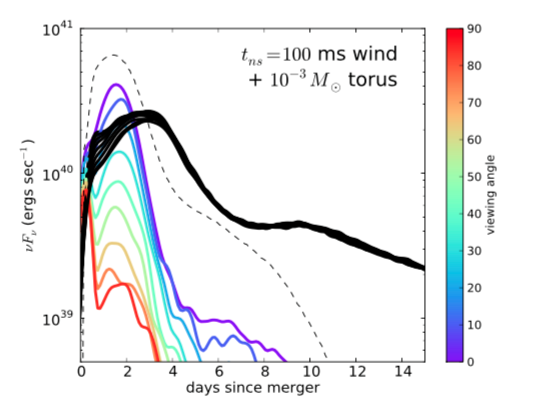
\includegraphics[scale=0.6]{figures/kilonova_lightcurves}
\caption{Kilonova light curves for a composite ejecta including a lanthanide-poor disk wind from a HMNS remnant with lifetime 100 ms, 
and a lanthanide-rich torus of dynamical ejecta. 
Colored curves show the optical light curves as a function of observer inclination from the rotation axis, 
while black curves show near infrared emission. Figure from \citet{2015MNRAS.450.1777K}.}
\label{fig:KNlightcurve}
\end{figure}

\subsection{Observational Evidence}

In 2013, \citet{2013Natur.500..547T} and \citet{2013ApJ...774L..23B} reported evidence 
that suggests a companion Kilonova to the short GRB 130603B (see figure \ref{fig:tanvir}).
GRB 130603B was detected on BATSE with a $T_{90}$ of about 0.18 s and a redshift $z$ = 0.356.
It was also detected by Konus-Wind with a duration $T_{90}$ of 0.09 s.
The localization of the GRB to its host galaxy was done by a optical afterglow detected at the William Herschel Telescope 2.7 hours after the event.
This optical afterglow faded away afterwards, marking the link to GRB 130603B.

\citet{2013Natur.500..547T} imaged the localization area with the Hubble Space Telescope (HST) during a whole orbit in two epochs, 
9 days after and 30 days after the burst. They used both the optical F606W filter (0.6 $\mu$m) and the nIR F160W filter (1.6 $\mu$m).
Using differential photometry (see section \ref{section:dia}) for the two epochs, they found a very faint excess of flux at the host galaxy.
Their photometry analysis gave a magnitude R606,AB > 28.25 (2$\sigma$ upper limit) and H160,AB = 25.73 $\pm$ 0.20.

\citet{2013ApJ...774L..23B} also imaged the area with HST for two different epochs, one 9.4 days after and another one \textasciitilde30 days later.
Using differential photometry, they found a point source 
with magnitude r = 21.56 $\pm$ 0.02 mag at 8.2 hr and r $\gtrsim$ 24.8 mag (3$\sigma$) at 32.2 hr.

Even though the source was very faint, the magnitude and color observed by HST 
were in accordance to the prediction of numerical merger models for a Kilonova.

\begin{figure}
\centering
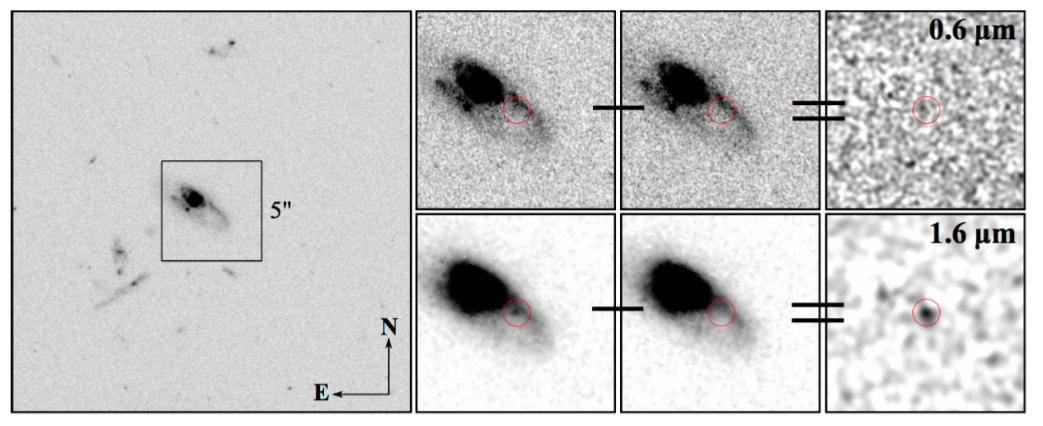
\includegraphics[scale=0.3]{figures/tanvir_kilonova}
\caption{HST imaging of the location of SGRB 130603B. The left-hand panel shows the host and surrounding field. The next panels show in sequence the first epoch and second epoch imaging, and difference (upper row F606W/optical and lower row F160W/nIR). From \citet{2013Natur.500..547T}.}
\label{fig:tanvir}
\end{figure}

There were two other searches for NIR emission for the afterglow of GRB 060614 by \citet{2015ApJ...811L..22J} and \citet{2015NatCo...6E7323Y}.
They are indicative of possible r-process emission of a Kilonova.

Finding a Kilonova companion to a GW NS-NS merger or BH-NS would be a direct confirmation of the association 
between Kilonovae, the r-process during a compact object merger, and the short kind of GRBs.


\subsection{Conclusion}

In summary, Kilonova emission is an ideal EM counterpart to the LIGO observations.
As previously said, unlike SGRBs, Kilonova emission is isotropic. 
Even though short GRBs emission is also present during the BNS merger, the r-process emission in the jet and other merger neutron ejecta, is fairly isotropic.
The chances to detect the GRB jet are very limited by the collimation of the jet and our line of sight, but r-process radiation is not. 

The Kilonovae are bright.
It was based on their derived peak luminosities, of approximately 1,000 times brighter than a nova, that Metzger et al. (2010) first introduced the term `kilonova' to describe this EM counterparts.

Another fundamental element that the multi-messenger astronomy contributes with,
is the identification of host galaxies.
The inference of the distance to the GW event using redshift of host galaxy will greatly reduce degeneracy in the GW parameter estimation,
especially of the binary inclination with respect to the line of sight.
It will also give a better estimate of the energies involved in the merger.
Other interesting environment properties can be derived from the Kilonova detection, like age of the stellar population and possible displacements due to SN birth kicks.

But most importantly, the merger of a binary system involving a NS is very complex and several kind of factors can effect the radiation pattern and light-curve of the Kilonova as well as the GRW waveform. 
The optical light curve can serve as a probe into the core and shed light to the intricacies and details of the merge process.

\begin{comment}

Rate of GRBs from NS-NS mergers is low, less than once per year all-sky. (e.g. \citet{2012ApJ...746...48M})
We should not expect the first --or even the first several dozen-- GW chirps from NS-NS/BH-NS mergers to be accompanied by a GRB.

Population synthesis models of field binaries predict GW detection rates of NS-NS/BH-NS mergers of about 0.2-300 per year, 
once Advanced LIGO/Virgo reach their full design sensitivities near the end of this decade (e.g. \citet{2010CQGra..27q3001A, 2015ApJ...806..263D}).
Empirical rates based on observed binary pulsar systems in our galaxy predict a comparable range, 
with a best bet rate of about 8 NS-NS mergers per year (\citet{2004ApJ...601L.179K, 2015ApJ...815...67K}).

\textcolor{red}{From here on, this is brought from the toros section}

Black Hole-Neutron Star (BH-NS) or Binary Neutron Stars (BNS) mergers are among the expected events detectable by the LVC. 
These highly energetic events will emit GW radiation in the frequency range of LIGO and Virgo sensitivity, strong enough to be detected up to a few hundreds Mpc of distance.
The precise maximum detection distance depends mainly of the masses involved in the merger, as well as other geometrical and spin parameters, but it sits at around 400 Mpc.

BNS and BH-NS mergers have long been proposed as the process leading to short-hard gamma-ray bursts (SGRBs) 
(\citet{1989Natur.340..126E, 1992ApJ...395L..83N}), but unfortunately this emission is beamed and thus can only be observed in a small fraction of the events.

Mergers with NS are also predicted to be accompanied by a more isotropic EM counterpart, commonly known as a `Kilonova'. 
Kilonovae are day to week-long thermal, supernova-like transients, which are powered by the radioactive decay of heavy, neutron-rich elements synthesized in the expanding merger ejecta (\citet{1998ApJ...507L..59L}). 

\end{comment}


%%%%%%%%%%%%%%%%%%%%%%%%%%%%%%%%%%%%%%%%%%%%%%%%%%%%%%%%%
%
%			TOROS
%
%%%%%%%%%%%%%%%%%%%%%%%%%%%%%%%%%%%%%%%%%%%%%%%%%%%%%%%%%
\chapter{The TOROS Project}

In 2011, scientists from the Center for Gravitational Wave Astronomy (CGWA) at 
The University of Texas at Brownsville (UTB) 
and the Observatorio Astronomico de Cordoba (OAC) and Instituto de Astronomia Teorica y Experimental (IATE) (the last two in Argentina)
established the TOROS project (\citet{2014EAS....67..357B})
to scan likely areas of the localization uncertainty sky map of the GW trigger, looking for possible optical counterparts.
%to respond to the LVC GW triggers with a wide field search for possible optical counterparts in likely areas of the localization uncertainty sky map.

%Motivated by complementing the LIGO observations in the electromagnetic (EM) side, Dr. Mario Diaz from UT RGV founded the TOROS project. TOROS (the Transient Optical Robotic Observatory of the South), has the main goal of scanning the uncertainty region of the LIGO localization map for GW events, with a wide field telescope and a large CCD pixel camera, searching for EM transients candidates for counterparts for such GW event.

TOROS stands for Transient Optical Robotic Observatory of the South,
and its original project consisted in the construction of an observatory site in Cordon Macon,
a mountain top at 4637 m above sea level, in the Andes mountain range in the north of Argentina.

Cordon Macon is a location with high quality seeing and excellent photometric quality.
The mean and median of the seeing measurements obtained at Macon are 0.70'' and 0.55'', respectively (\citet{2009BAAA...52..285R}). 
Several sites within the area around Cordon Macon were considered for the location of the European Extremely Large Telescope, including a site on the Macon Ridge itself.
%It will also link the network of observatories to the sky in the Southern hemisphere.

The proposed TOROS telescope would have a 0.6 m aperture and a 9.85 sq. deg. field of view.
When fully operational it is planned to have three basic modes of operation:
follow up of GW triggers; 
follow up of gamma-ray burst triggers from Fermi, Swift, and other missions; 
and baseline imaging of the entire surveyable area.

It is also included in the full project the inclusion of a data reduction and processing pipeline for transient detection, as well as a database for the dissemination of catalogs and triggers.

While the original project remains on hold awaiting for proper financing of the facility, several other institutions showed interest to participate as well.
This broadened the TOROS project into a wider collaboration of telescopes instead of the single telescope in Argentina that was originally envisioned.

%The collaboration has now partners in Mexico, and the Gemini spectrograph as well as the telescopes in Chile and Cordoba previously mentioned. \textcolor{red}{Use this paragraph to include all the participating institutions}

Whether it be the original design or the new dynamic proposed by the enlargement of the collaboration, 
the interesting targets to TOROS remain to be mergers with at least one NS, because of its several radiation messengers.


%%%%%%%%%%%%%%%%%%%%%%%%%%%%%%%%%%%%%%%%%%%%%%%%%%%%%%%%%
%
%	                     PIPELINE
%
%%%%%%%%%%%%%%%%%%%%%%%%%%%%%%%%%%%%%%%%%%%%%%%%%%%%%%%%%

\section{Building a software pipeline for TOROS}

Since the ultimate goal of the TOROS Project is the robotization of the telescope,
it is important to have in place a software `pipeline' that accompanies the process
at all stages, from receiving the alert to propose new transient candidates.

The whole operation of TOROS processing can be divided in several stages
as in the diagram of figure \ref{fig:flowchart}.

\begin{figure}
\centering
\scalebox{0.8}{
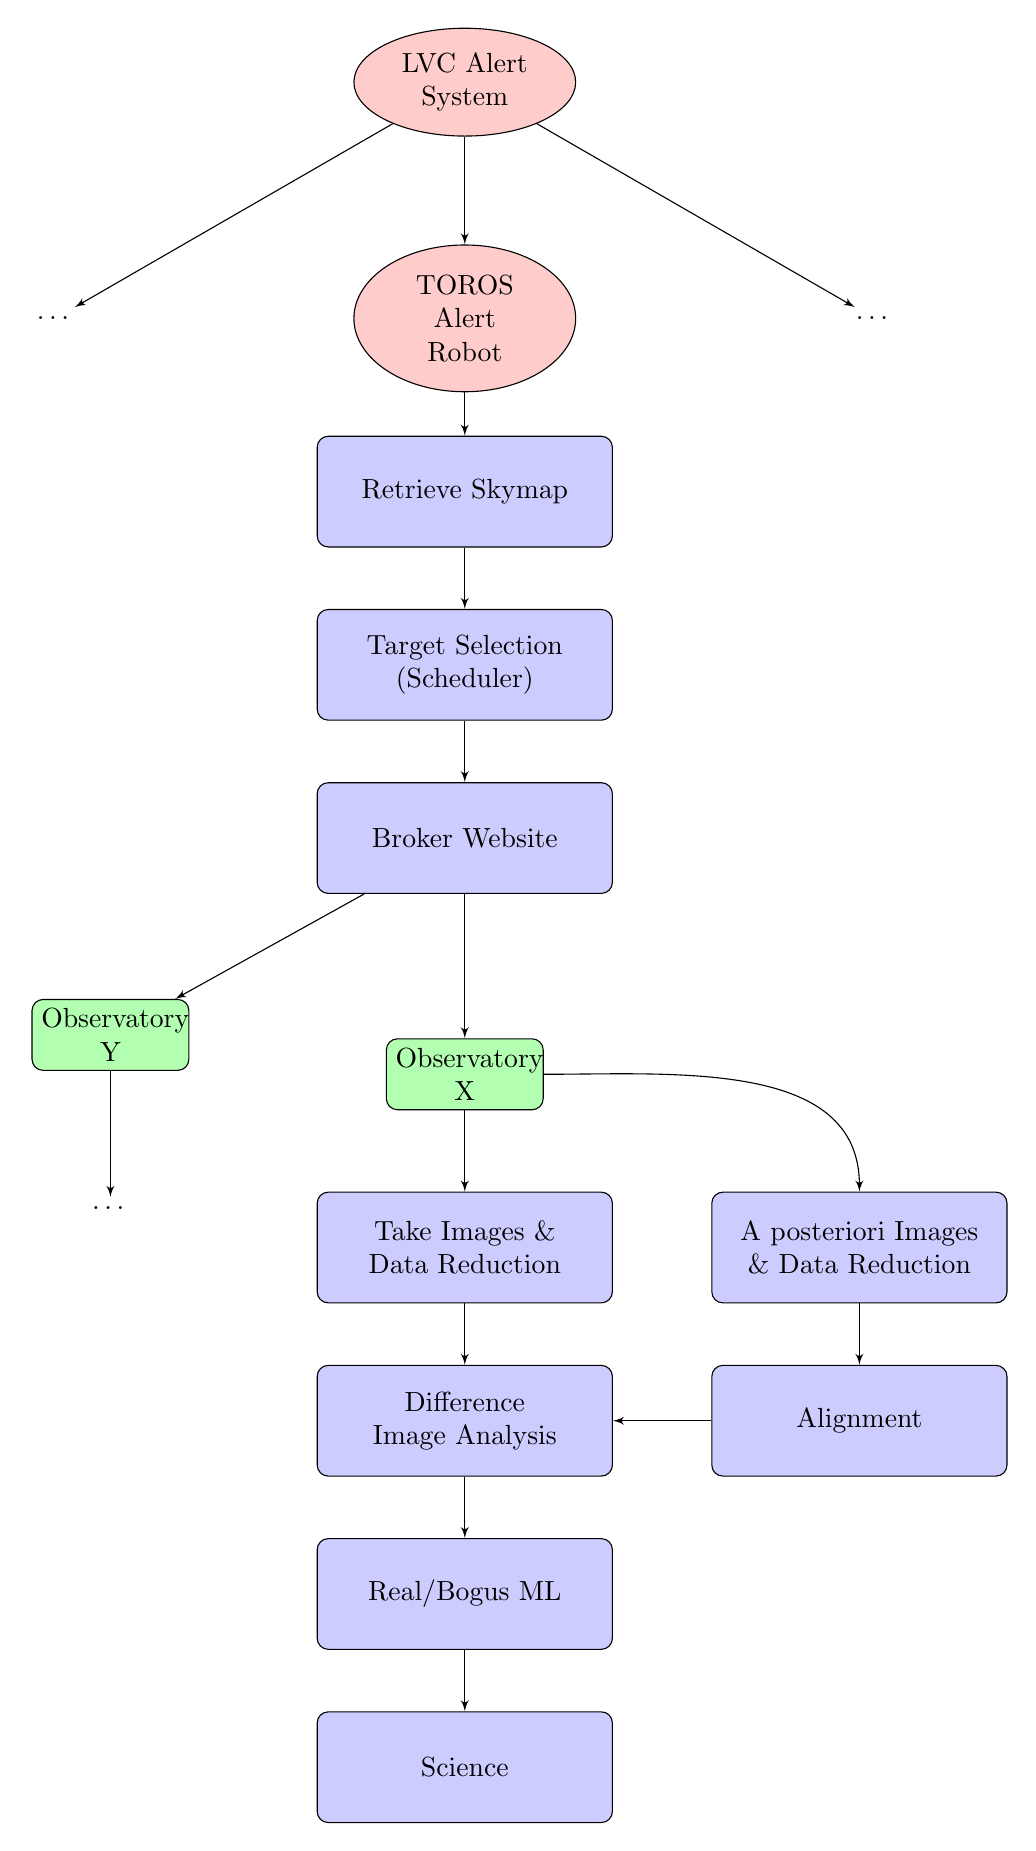
\begin{tikzpicture}[node distance = 2.2cm]
    % Place nodes
    \node [cloud] (ligo) {LVC Alert System};
    \node [cloud, below of=ligo] (robot) {TOROS Alert Robot};
    \node [xshift=-3cm, left of=robot] (collabx) {\ldots};
    \node [xshift=3cm, right of=robot] (collaby) {\ldots};
    \node [block, below of=robot] (skymap) {Retrieve Skymap};
    \node [block, below of=skymap] (targets) {Target Selection (Scheduler)};
    \node [block, below of=targets] (broker) {Broker Website};
    \node [obse, below of=broker] (obsx) {Observatory X};
    \node [obse, left of=obsx, xshift=-1.5cm, yshift=0.5cm] (obsy) {Observatory Y};
    \node [below of=obsy] (ldots) {\ldots};
    \node [block, below of=obsx] (images) {Take Images \& Data Reduction};
    \node [block, right of=images, xshift=8em] (refimages) {A posteriori Images \& Data Reduction};
    \node[block, below of=refimages] (align) {Alignment};
    \node [block, below of=images] (dia) {Difference Image Analysis};
    \node [block, below of=dia] (realbogus) {Real/Bogus ML};
    \node [block, below of=realbogus] (science) {Science};
    % Draw edges
    \path [line] (ligo) -- (robot);
    \path [line] (ligo) -- (collabx);
    \path [line] (ligo) -- (collaby);
    \path [line] (robot) -- (skymap);
    \path [line] (skymap) -- (targets);
    \path [line] (targets) -- (broker);
    \path [line] (broker) -- (obsx);
    \path [line] (broker) -- (obsy);
    \path [line] (obsy) -- (ldots);
    \path [line] (obsx) -- (images);
    \path [line] (obsx) to[out=0, in=90] (refimages);
    \path [line] (images) -- (dia);
    \path [line] (refimages) -- (align);
    \path [line] (align) -- (dia);
    \path [line] (dia) -- (realbogus);
    \path [line] (realbogus) -- (science);
\end{tikzpicture}
}
\caption{The pipeline flowchart.}
\label{fig:flowchart}
\end{figure}

The pipeline is written entirely in Python, following the latest trend in Astronomy.

Python is an interpreted language like Java, as opposed to other compiled languages like C/C++ or Fortran.
While this may seem a disadvantage, it becomes very useful to quickly prototype and integrate projects into working systems.
Python code can be executed line by line in command line interpreters, in a cell by cell manner like MATLAB\footnote{https://www.mathworks.com/products/matlab.html}
or as a script.

Python is fully Object-Oriented but it also allows to encapsulate functionality into modules or packages that can be imported into your own project.
This modularity makes it very easy to expand an existing project by adding external functionality (much like with libraries in compiled languages)
in a transparent to the user in a one-line import.

Another advantage of python is the ease to install these packages. Python counts with a standard package installer that takes cares of dependencies (compilable or not).
These are just a few features of the language ecosystem that it's making Python gain traction in the Astronomy community.
Python along with tools like git (and the github repository website) and virtual environments make Python projects reproducible and installable in almost any Unix-like system with minimum effort.

Python popularity in the science community started with the introduction of two main packages: numpy and scipy (which collected the linear algebra routines found in BLAS/LAPACK).
After this, another project ``astropy'' began porting popular IRAF methods to python. 
Nowadays the list of Python scientific packages is too long to enumerate, but we describe some useful packages and modules on table \ref{pythonpackages}
This project itself spun the creation of two new modules astroalign and ois (see sections \ref{section:astroalign} and \ref{section:ois}) to align stellar images and perform image subtraction respectively.

\begin{table}
\centering
\begin{tabular}{l m{10cm}}
\hline
Package Name & Description \\ \hline
NumPy & Collection of Numerical routines for Python \\ \hline
SciPy &  Python-based ecosystem of open-source software for mathematics, science, and engineering. \\ \hline
Astropy &  ``The Astropy Project is a community effort to develop a single core package for Astronomy in Python and foster interoperability between Python astronomy packages.'' \\ \hline
photutils & Tools for detecting and performing photometry of astronomical sources \\ \hline
sep & A rewrite of SExtractor. A C library and Python module for Source Extraction and Photometry \\ \hline
reproject & Implements image reprojection (resampling) methods for astronomical images (uses WCS data) \\ \hline
matplotlib & General visualization and graphing outines \\ \hline
APLpy & Module based on matplotlib, to produce publication-quality plots of astronomical imaging data in FITS format \\ \hline
scikit-learn & Tools for data mining and data analysis \\ \hline
PyGCN & Module to connect to the GCN/TAN network \\ \hline
Django & Web Framework for backend web development \\ \hline
\end{tabular}
\caption{Some of the scientific packages available for Python}
\label{pythonpackages}
\end{table}

In the following sections, I explain the different components of the pipeline diagram.

\section{TOROS Alert Robot}

\begin{comment}
\textcolor{blue}{LSST will send out public VOEvents describing the millions of transient and variable detections each night. 
Huge databases (upwards of 12 PB for LSST at the end of its 10 year survey) of objects and all of their detections will be created and available for queries. 
Users will be able to use this database to identify and classify the target samples of interest to them, as well as access the VOEvent stream to get real-time updates on targets.}

\textcolor{blue}{the IVOA has settled on a flavor of XML called VOEvent for the transmission of astronomical events, and processing those would need XML streaming and filtering technologies.}
\end{comment}


The first step of the process starts with the alert receiver robot.

The alert receiver is hosted in a virtual machine server provided by UTRGV IT Services.
It is a Python script that runs uninterruptedly waiting for a detection alert from the 
Gamma-Ray burst Coordinates Network (GCN) and the Transient Astronomy Network (TAN),
a service of NASA delivered on a specific port reserved for this purpose.

The GCN/TAN network is a distribution network of transient event notices dependent on Goddard NASA.
As its name suggests, it was primarily intended for the distribution of GRBs detection notices
from space telescopes like Fermi, Swift and other spacecrafts, to the rest of the Astronomy community. 
Later on, they allowed for the dissemination of other types of interesting transient phenomena.
Most notices are sent in real-time, while the event is still ongoing, 
others are delayed due to telemetry down-link delays.

The subsequent reports of follow-up observations made by ground-based observers, are done by submitting circulars to that same site.
This makes the GCN/TAN network \emph{``a one-stop shopping network for follow-up sites and GRB and transient researchers.''}

The LIGO-Virgo Collaboration makes use of the GCN network to disseminate GW detection
notices to the participating observatories searching for EM counterparts.

The notice comes in the form of a Virtual Observatory Event (VOE) file,
and it is distributed as a message to predefined static IPs and ports,
using the VOEvent Transport Protocol.

The VOEvent Transport Protocol is a simple TCP-based protocol for transporting VOEvent messages from authors, through brokers, to subscribers.

VOEvent is the International Virtual Observatory Alliance\footnote{http://ivoa.net} (IVOA) recommended mechanism for describing astronomical transients.
It has been adopted as an international standard.
According to its main website\footnote{\href{http://wiki.ivoa.net/twiki/bin/view/IVOA/IvoaVOEvent}{http://wiki.ivoa.net/twiki/bin/view/IVOA/IvoaVOEvent}},
a VOEvent is an XML file notice that ``\emph{defines the content and meaning of a standard information packet for representing, transmitting, publishing and archiving information 
about a transient celestial event, with the implication that timely follow-up is of interest.}'' 

In our case, we registered two static IPs with GCN, one in Texas at UT RGV and another one for Cordoba in Argentina at IATE Institute.
Only the one in Texas is functional at the moment.

The VOEvent is received by a continuously running Python script that listens on the specific port and creates an alert email involving the heads and some staff at each TOROS partner.

The PyGCN module developed by Leo Singer, handles the reception GCN notices from LVC using the TCP protocol.
Once a notice is received, PyGCN calls a call-back function that performs the rest of operations on the notice.

The first thing the listener script does is sending an email with the VOEvent attached to a list of recipients in the TOROS collaboration.

The second thing, is parsing the XML file.
The VOEvent comes in the Extensible Markup Language (XML) format, a well established worldwide standard in web technologies.
The XML schema provides a structured way to build a nested hierarchy of elements, to attach attributes to those elements, and to assign values to them. 
The structured text is parsed with a Python native package to scavenge the relevant information from within the nested hierarchy.
Some of the information contained in the VOEvent are listed in table \ref{voeventinfo}

\begin{table}
\centering
\begin{tabular}{| l | >{\itshape}m{9cm}|}
\hline
GraceID & Identifier in the Grace Database \\ \hline
AlertType & VOEvent alert type. It could be any of `Initial' or `Update' \\ \hline
SKYMAP\_URL\_FITS\_BASIC & Provides the URL of the location probability map for LIGO/Virgo GW event detections (FITS format). \\ \hline
SKYMAP\_URL\_PNG\_BASIC & Provides the URL of the location probability map for LIGO/Virgo GW event detections (PNG format). \\ \hline
ProbHasNS & Probability that at least one object in the binary is less than 3 solar masses \\ \hline
ProbHasRemnant  & Probability that there is matter in the surroundings of the central object \\ \hline
ISOTime & The time of the event in ISO format \\ \hline
\end{tabular}
\caption{A few examples of the kind of information provided in the VOEvent notice.}
\label{voeventinfo}
\end{table}

Once information is parsed, a second email is sent with the relevant information from the VOEvent along with the skymaps retrieved from the provided URL
(see SKYMAP\_URL\_FITS\_BASIC on table \ref{voeventinfo}) and its corresponding PNG file. 

The third step in the process, is to generate a list of targets of observations for each observatory and upload them to the broker website.
Although this is done by the alert receiver robot, we explain these steps in more depth in the following sections.

\section{Skymaps}

LIGO relies on triangulation to localize the originator of the signal in the sky.
With two detectors running, the localization will contain a degeneracy separated by 180${}^{\circ}$ 
and it may not be a simply connected region.
A third detector would break the degeneracy and cut in a third the localization uncertainty area (\citet{2014ApJ...795..105S}).

Soon after a coincident detection on the operating detectors, 
a rapid sky localization is made with BAYESTAR (\citet{2016PhRvD..93b4013S}).
BAYESTAR is a rapid Bayesian position reconstruction code that will produce accurate sky maps in less than a minute after any BNS merger detection.

The rapid response is achieved by using only information of the coincident triggers: the phases, times of arrival and amplitudes, 
along with prior probability distributions of source parameters.
It will not use the GW parameters from the reconstruction of the wave-form, like costly post-Newtonian GW wave-form calculations.

LIGO has other three localization estimation codes: LALINFERENCE\_MCMC, LALINFERENCE\_NEST and LALINFERENCE\_BAMBI.
The LIGO Algorithm Library (LAL) is a collection of routines for various pipelines inside LIGO for which LAL Inference is specific to parameter estimation.
These three codes are stochastic MCMC samplers that estimate the full GW parameter space, 
they can give a localization skymaps by marginalizing over every parameter that is not the sky location.
The LALINFERENCE localization estimations may take days to complete, and weeks if the spin of the compact objects is taken into account.
These are far more computationally expensive than BAYESTAR, but they will improve the estimations for the localization, 
especially when the GW signal is very weak in one detector.

Another LAL code for unmodeled bursts is the LAL Inference Burst, or oLIB (\citet{2015arXiv151105955L}).
This LAL code, unlike the others in LAL Inference, has low latency.
The algorithm relies in excess of power detection; coincidence between different detectors; and analysis of coincident events using Markov Chain Monte Carlo Bayesian inference.

The coherent WaveBurst (cWB) (\citet{2016PhRvD..93d2004K}) is another real-time detection and localization estimation code
that makes little to no assumptions on source models.
To estimate localization, they use a maximum likelihood approach on their calculated likelihood for bursts, restricted to the $(\theta, \phi)$ variables for positioning.
The code allows for very low latency (only a few minutes).

At the time of the detection, observatories will rely on the position estimation of BAYESTAR, cWB or oLIB.
By the time the LALINFERENCE maps are released, most of the observations will be already done.

The retrieval of the low latency sky maps is done through authenticated HTML GET requests to the Grace Database of the GCN/TAN website.

\section{Target Selection} \label{targetselection}

The target selection is done with a separate module imported from the alert receiver robot.
Having it in a separate module allows us to run it independently, in case of failure of the robot.

The skymaps provided with the alert typically cover an order of \textasciitilde200 square degrees for the 60\% confidence region (\citet{2014ApJ...795..105S}).
For telescopes that have not wide enough field of views to tile the region in a few pointings, it becomes an absolute necessity 
to adopt some kind of target selection strategy to maximize the chances of discovery.

The goal is to prioritize pointing directions in order of interest.
The important role of galaxy catalogs was noted early in \citet{2011CQGra..28h5016W}, where they presented
the Gravitational Waves Galaxy Catalog (GWGC).
The GWGC catalog is a homogeneous list of 53,255 galaxies within 100Mpc.
It is a compilation from 4 different catalogs: an updated version of the Tully Nearby Galaxy Catalog,
the Catalog of Neighboring Galaxies, the V8k catalogue and HyperLEDA.

GWGC contains information on sky position, distance, blue magnitude, major and minor diameters, position angle, and galaxy type.
Also included in the catalog are 150 Milky Way globular clusters.

The authors claim that GWGC is more complete --within 100 Mpc-- than other catalogs,
due to their use of more up-to-date input catalogs
and the fact that they don't make a blue luminosity cut.

In \citet{2014ApJ...784....8H} they find that the use of galaxy catalogs can improve success rates by \textasciitilde10\% 
to a factor of 4 relative to follow-up strategies that do not utilize this kind of catalogs.

Our target selection (scheduler) module makes use of the sky-map provided in the alert notice and the 
GWGC catalog.

%Another catalog along these lines is the Glade GW Catalog. Glade Catalog has xxxx galaxies listed, this many more than CWGC and extends up to XX Mpc.
%Nonetheless many distances are inferred by Machine Learning Methods, and completitude of the Catalog... bla bla

The target selection for our optical search is based on three main criteria: 
the localization (un)certainty on the target pixel in the all-sky map given by LIGO at the time of the alert,
the visibility of the targets at the moment of the event by our several telescopes, 
and several filter cuts on distance, blue luminosity and apparent magnitude.

For the selection of targets we first apply filters to the objects in the GWGCatalog of the intrinsic parameters 
(Apparent Magnitude, Distance and Absolute Magnitude). 
We then exclude those objects with Right Ascension values that make them not observable for the time of the year.
With those filtered objects, we run for each observatory further filters on Declination visibility, appropriate to the location of the specific telescope.
The remaining objects are ordered according to the probability of the skymap pixel in their location 
and we assign a few dozens of the most likely to each observatory to be followed-up.

The parameter cuts can be fixed in a separate configuration file and loaded at the time of execution.

This marriage between GW and Optical parameters of observability ensures the targets are visible at each telescope site, 
and that they have some significant probability of being the host.

\section{The Broker} \label{section:broker}

Once the list of targets is done, we need to communicate the targets to each telescope.
This is done through a broker website written in Python using the Django\footnote{\url{https://www.djangoproject.com}} web framework (see figure \ref{fig:brokerhead})
and a light database on Sqlite 3.

\begin{figure}
\centering
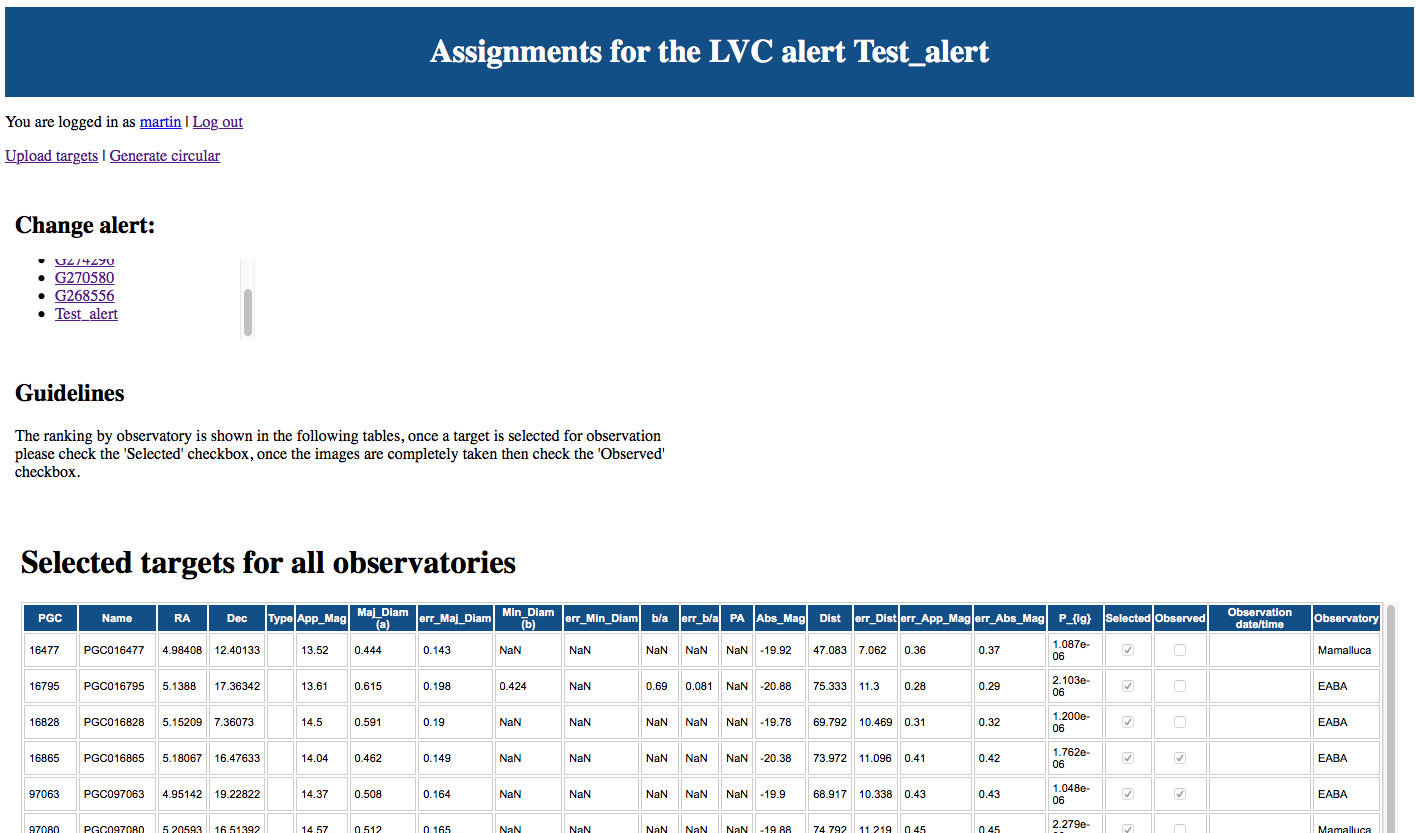
\includegraphics[scale=0.3]{figures/broker_header}
\caption{A portion of the Broker website with target assignments.}
\label{fig:brokerhead}
\end{figure}

\begin{figure}
\centering
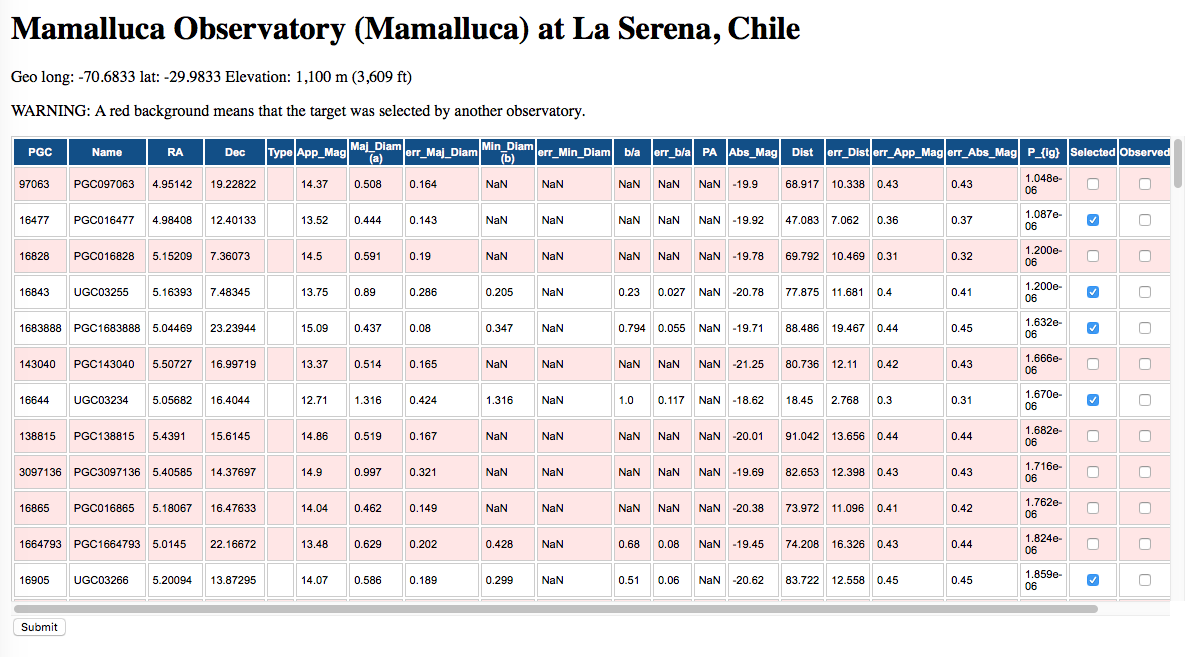
\includegraphics[scale=0.4]{figures/broker_obsdetail}
\caption{An example of a detail table of targets assigned to the Mamalluca Observatory.}
\label{fig:brokerdetail}
\end{figure}

Sqlite provides a lightweight database solution that does not require complex server-client operations, and it stores all data in a simple file.
Thus, the database is easy to browse and modify.
The database handles information for the GW Galaxy Catalog, the user information as well as permissions and login information,
and data about the observatories.

Each telescope representative has assigned a username and password to access a 
website\footnote{\url{http://toros.utrgv.edu/winnow/broker/}} hosted in UT RGV servers.
This website has a simple interface of tables for each observatory and a list of targets observable from each location, obtained by the target selection method on the previous step.

Each telescope admin then selects targets from the list, to reserve them for his or her observatory (see figure \ref{fig:brokerdetail}). 
The website enforces that the list of targets be unique and that no two observatories are observing the same target.
It does so, by ignoring targets previously selected by others on the query.

Each observatory then carries the observations for the successive nights 
and will mark the targets on their observatory table once they are observed.

The website can also output a circular draft of all the targets observed by each telescope 
to be submitted to the GCN/TAN website for the rest of the community.

\section{Data Reduction}

The data reduction step of the pipeline is specific to the data processing techniques used in each observatory 
and we will not cover them on this section.
Instead, for the purpose of testing the Optimal Subtraction and Real-Bogus Classifier steps, we discuss here the preparation of a test image set 
from the Chinese Telescope ARray, CSTAR.

\subsection{CSTAR}

CSTAR is a set of Chinese telescopes on the Antarctic ice cap (\citet{2010RAA....10..279Z}).
CSTAR was deployed in Dome A on the Antarctic Plateau (87.3667${}^{\circ}$S, 77.3500${}^{\circ}$E),
and had several observation runs from 2008 to 2011 when it was sent back to China for upgrades.

Dome A provides unique observation conditions.
It is located at an altitude of 4,200 m and its atmospheric conditions are excellent giving less than 0.4 mag extinction for 70\% of the time.
The temperature ranges from -80${}^{\circ}$C to -60${}^{\circ}$C and it has uninterrupted dark conditions for 6 months.

The image set that we used was taken during the Antarctic winter of 2010.
The original array of CSTAR telescopes consisted of four similar telescopes with different filters on them.
Three of them had standard SDSS \emph{gri} filters and the fourth one was a \emph{clear} filter.
Only the images from filter \emph{i} in 2010 were usable since the other 3 telescopes failed to return data.
The telescopes are a Schmidt-Cassegrain with 145 mm aperture and a 20.1 square degrees field of view.
They are equipped with an ANDOR DV435 1K$\times$1K frame-transfer CCD with a pixel size of 13$\mu$m.
The telescopes do not track and have no moving parts.
They are pointed to the South Celestial Pole and the exposure time is such that the drift time covers less than a pixel.
The CSTAR 2010 \emph{i} set has a median exposure time of 42 s.

The entire data set for the winter of 2010 consists of 251,818 images spanning from April 30 2010 to September 27 2010.
Since the amount of data is so large, for the purpose of training, we created a subset of 626 images, 
with a cadence of about an hour during the best seeing month of June (May 31st to June 30th, 2010). 
The subset was named `cstar\_june\_selection'. 
The first 10 images of this set (named cstar\_june\_01) is used for training purposes and the rest can be used to search for transients. 

The images we worked with were preprocessed, i.e. they were bias and flat corrected.
The CCD had a few dead columns and rows and bright stars suffer from `bleeding' (see figure \ref{fig:bleeding}) even though they have low exposure time.
This bleeding is very significative for bright stars and less so for dimmer stars but still present nonetheless.

\begin{figure}
\centering
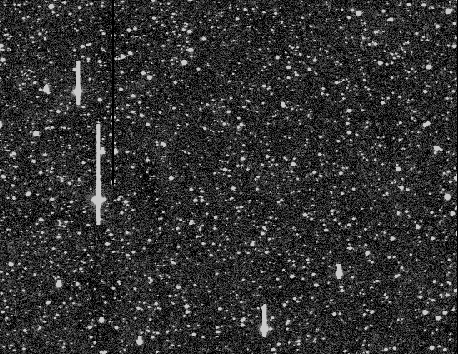
\includegraphics[scale=0.4]{figures/bleedingexample}
\caption{An example of the bleeding of bright stars on the CSTAR image set.}
\label{fig:bleeding}
\end{figure}

The bled stars were covered with the median and a separate mask was created for the covered pixels for future reference.
This pixel mask also includes defective pixels (dead lines and columns in the CCD).

The date-time information on the header was also updated according to \citet{2013AJ....146..139W}.
The GPS receiver in the telescope to maintain time synchronization had a communication problem with the main computer that caused a drift in the time stamp of the FITS images.

Because the CSTAR telescope points to the South Celestial Pole and has no tracking, the images show the Earth rotation and minor translations with respect to each other.
We then re-aligned the reference image to each one of the 626 image in the cstar\_june set using the package `astroalign' (see section \ref{section:astroalign}).

\section{Optimal Subtraction} \label{section:dia}

Searches for time-varying and position-changing objects are undertaken by comparing a reference image of a particular region of the sky 
with a second image taken at the moment in which we are interested. 
The two images have to be aligned pixel by pixel and then subtracted to reveal any changes in light.
In our case, we used a reference image constructed by stacking several CSTAR images from the best-\emph{seeing} month of June 
and then we aligned this to each of the frames in the data set.

To make a suitable subtraction of the two images, one has to match the frames to exactly the same \emph{seeing}. 
Image Difference, also known as Optimal Subtraction or Differential Photometry, is a technique to find a convolution kernel that best describes 
(in some minimization sense) the change in point spread function between the images. 
The idea is to degrade the good \emph{seeing} image ---our reference image--- to match the \emph{seeing} of our second image. 
Finding the proper convolution kernel can be a delicate operation and there's plenty of literature on the subject. 
Methods range from PSF modeling through common Gaussian profiles; to unmodeled PSF's; to Information Theory; and Fourier Domain.

The general problem can be stated as follows. 
We have an image $I$ and a reference image $R$, for which we want to find a convolution kernel $K$ such that 
the convolution of $R$ with $K$ best approximates $I$.

\begin{align} \label{thdiaeq}
I(x,y) & \approx (R \mathbin{*} K)(x,y) \\
 & \approx \int \mathrm{d}u \mathrm{d}v {R (u,v) K(x-u,y-v)}
\end{align}

The integral symbol has to be understood in practice, as a sum over all the pixels on the image. 

The kernel $K$ will try to correct for the PSF difference between the two images.
It's worth noting here, that even though it could be practical to the reader to think so, 
the kernel $K$ is neither the PSF of the reference nor the PSF of the image.

Ideally, the reference image is the one with the best \emph{seeing}, 
because it can be done by median-stacking good images, or using Speckle Imaging (\citet{1978JOSA...68.1651F}) or some other method.

The inversion problem \ref{thdiaeq} can be computationally very expensive to invert directly.

The first attempt at image subtraction goes back to \citet{1995ASPC...77..297P}. 
They solved the equation in Fourier domain, where the convolution transforms into a simple multiplication.

\begin{align}
\tilde{I} = \tilde{R} \tilde{K} \\
K = \mathcal{F}^{-1} \left \{ \tilde{I} / \tilde{R} \right \}
\end{align}

Unfortunately, the solution is not numerically stable because it is very sensitive to high frequency noise.
Even with moderate levels of noise the results were not always good.

\citet{1998ApJ...503..325A} were the first to propose a solution in image space (as opposed to Fourier space). 
%They also summarize previous efforts in their introduction and references therein. 
In their paper, they propose an optimization solution by converting the convolution inversion into a linear problem.
First, they decompose the kernel into a linear combination of ``\emph{basis}'' kernels $B$.

\begin{equation} \label{thkernel_linear}
K(u,v) = \sum_{i} a_{i} B_{i}(u,v)
\end{equation}

These $B_{i}$ could in principle be any reasonable set of functions. 

Using this linear combination, the convolution will be

\begin{align}
(R \mathbin{*} K)(x,y) & = \sum_{i} a_{i} \left( R \mathbin{*} B_{i} \right)(x,y) \\
 & \equiv \sum_{i} a_{i} C_{i}(x,y)
\end{align}

where the last line defines $C_{i}(x,y)$.

With this decomposition, we can find the set of $a_{i}$ that minimizes the square difference over all pixels.
Define a cost function $Q$:

\begin{align}
Q &= \int \left( I(x,y) - (R \mathbin{*} K)(x,y) \right)^2 \\
 & = \int \left( I(x,y) - \sum_{i} a_{i} C_{i}(x,y) \right)^2, \nonumber
\end{align}

and let's minimize $Q$ over the set of $a$'s:

\begin{align}
\frac{\partial Q}{\partial a_{i}} = & 2 \int \left( I(x,y) - \sum_{j} a_{j} C_{j}(x,y) \right) C_{i}(x,y) 
\end{align}

Setting the last equation to zero, gives us:

\begin{align}
\sum_{j} a_{j} \int \left( C_{j}(x,y)  C_{i}(x,y) \right) =  \int I(x,y) C_{i}(x,y) 
\end{align}

Which we can write more succinctly as a matrix equation:

\begin{align} \label{thmatrix_eq}
\sum_{j} M_{ij} a_{j}  =  b_{i}
\end{align}

where

\begin{align} \label{thmatrix_def}
M_{ij}  &=   \int  C_{i}(x,y)  C_{j}(x,y) \\
b_{i} &=  \int I(x,y) C_{i}(x,y)  \nonumber
\end{align}

We can find the coefficients $a_{i}$ of the optimal kernel for the subtraction by inverting the system \eqref{thmatrix_eq}--\eqref{thmatrix_def}.

This very simple description captures the essence of a collection of algorithms that try to degrade the reference to match the image to subtract.
For a more extended discussion of this method and enhancements, we refer the reader to appendix \ref{appendix:dia}.

\citet{1998ApJ...503..325A} were the first to introduce this least-squares method to find an optimal image. 
They propose the use of multi-Gaussian functions with modulating polynomials as the kernel basis.

\begin{equation}
B_{n,d_n^{x}, d_n^{y}}(u,v) = e^{-(u^2+v^2)/2 \sigma_n^2} \times u^{d_n^{x}} v^{d_n^{y}}
\end{equation}

This basis works well when the PSF differences are approximately Gaussian, but in many situations the modulated Gaussian ansatz can be too restrictive.
Many PSF differences can not be modeled accurately this way, especially when there is very little difference between the image and its reference.
Another drawback is that the method can not fit for the $\sigma$ spread for the Gaussian functions and it has to be determined empirically from the data.

\citet{1998ApJ...503..325A} also introduced the simultaneous fit of background differences between the images.
Background estimation can be done previous to the subtraction or be included in the least-squares optimization.

In \citet{1998ApJ...503..325A} and \citet{2000A&AS..144..363A}, they also discuss the issue of PSF spatial variation.
The spatial variation is accounted for by further expanding each coefficient into a polynomial on the $(x, y)$ position on the image.
This makes the number of spatial dependance coefficients proportional to the original number of free parameters.
The introduction of yet more coefficients to adjust could make the method computationally prohibitive.
In \citet{2000A&AS..144..363A}, they propose an approximation to the problem using for the calculation 
only pixels on \emph{stamps} around sources and considering a nearly constant PSF on each stamp.

HOTPANTS (\citet{2015ascl.soft04004B}) and its predecesor ISIS (\citet{2000A&AS..144..363A}) are implementations of this method written in C.

\citet{2008MNRAS.386L..77B} proposed a similar method in which every pixel of the kernel is fit independently.
This is equivalent to choosing a basis of Kronecker Delta centered on each pixel.
The obvious advantage of this method is the great flexibility of the kernel shape.
This method can account (and correct) for small misalignments of the order of the kernel side.
%On the down side, the kernel shape is more sensitive to the noise outside the sources.
The cost to pay for the great flexibility in the kernel is the number of parameters to fit. 
They are significantly more than those of \citet{1998ApJ...503..325A} growing with the square of the kernel side.
%this results in that the multi-Gaussian basis can be significantly faster.

The \citet{2008MNRAS.386L..77B} method can also accommodate for a simultaneous fit of background and a spatial varying kernels.
To tackle the problem of PSF spatial variability he proposes dividing the image on a grid and perform a subtraction on each grid element.

In \citet{2008PASP..120..449M} they propose a method similar to \citet{1998ApJ...503..325A} with the use of \emph{stamps} to deal with PSF variation.
It's worth noting that introducing new coefficients for space variation is more costly on the Delta basis because of the larger number of original variables to fit in the kernel.

One particular problem with all these methods based on least-square optimization, 
is that they can be fooled with saturated stars and bad pixels on the image.
To avoid this, one can use a mask to exclude certain pixels from the calculation. 
For a more complete description of the treatment of bad pixels, see appendix \ref{appendix:dia}.

The bottleneck on these methods is the calculation of the matrix to invert. 
The inversion itself can be done very quickly with any algebra package,
but the number of operations for each element of the matrix system scales quadratically with the number of free parameters.
This is something to take into account when choosing the number of Gaussians and the polynomial degree or the kernel side for the Delta basis.

The implementation of these set of algorithms spun the creation of a new Python module named \emph{ois}\footnote{\url{https://github.com/toros-astro/ois}}.
For more details on the \emph{ois} Python implementation we refer the reader to section \ref{section:ois}.

For our set of images, I applied the \citet{2008MNRAS.386L..77B} method on a 4$\times$4 grid.
We also simultaneously fit and subtracted a third degree polynomial background.
We used a kernel side of 11 pixels, which correspond to 2.9' aperture on the sky. 
This is more than enough to accommodate for PSF differences: the FWHM from a typical image is only a few pixels wide.

Figures \ref{fig:subtraction} and \ref{fig:subtdetail} show an example of a difference image, 
and its pixel value histogram in figure \ref{fig:subthist}.

The optimal convolution kernels for each of the grid element, for a typical subtraction is shown in figure \ref{fig:kernels}.
A simultaneously polynomial fit to the background is shown on figure \ref{fig:bkgdetail}.


\begin{figure}
\centering
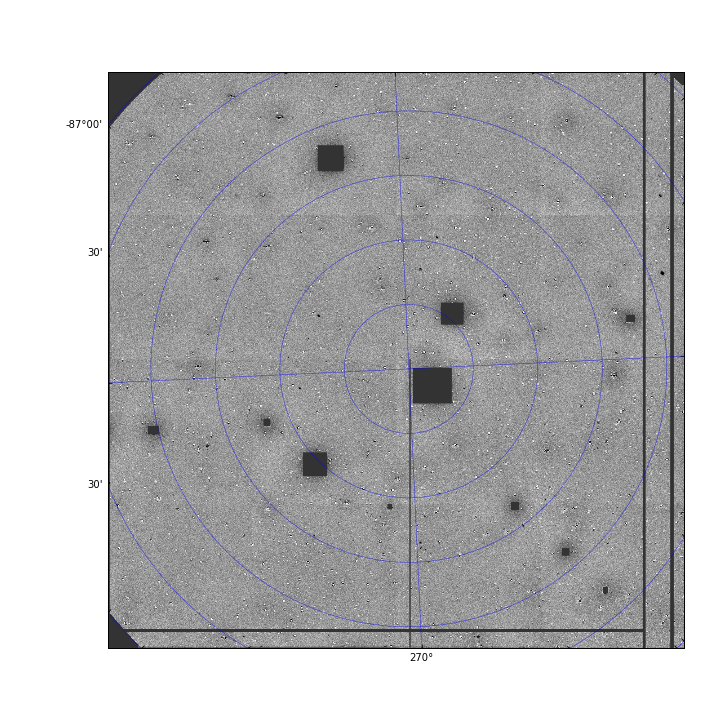
\includegraphics[scale=0.6]{figures/subtwaxes}
\caption{A typical subtraction image. The axis are added to show the position on the sky.
Also superimposed are marked in dark grey the masking on some bled stars and bad columns and rows.}
\label{fig:subtraction}
\end{figure}

\begin{figure}
\centering
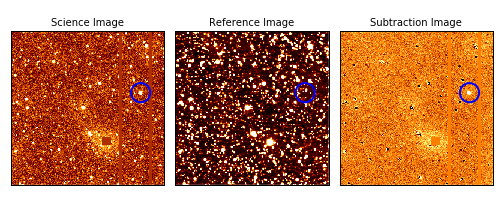
\includegraphics[scale=1.0]{figures/subtdetail}
\caption{A detail of the subtraction image showing an excess of light (blue circle) on the subtracted image.}
\label{fig:subtdetail}
\end{figure}

\begin{figure}
\centering
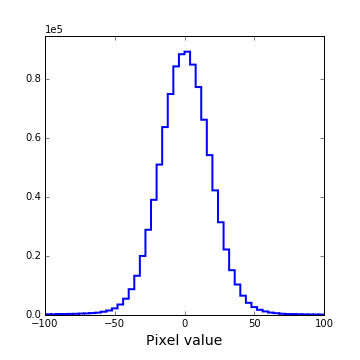
\includegraphics[scale=0.6]{figures/subthist}
\caption{Histogram of the subtraction (not all pixel values shown).
The pixel values are distributed around zero.}
\label{fig:subthist}
\end{figure}

\begin{figure}
\centering
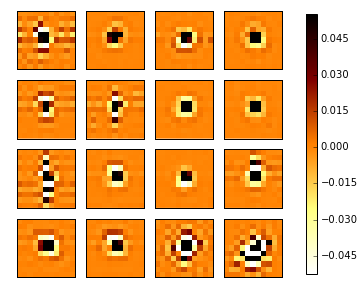
\includegraphics[scale=0.6]{figures/kernels}
\caption{The optimal convolution kernels for the subtraction on each of the regions of the grid.}
\label{fig:kernels}
\end{figure}

\begin{figure}
\centering
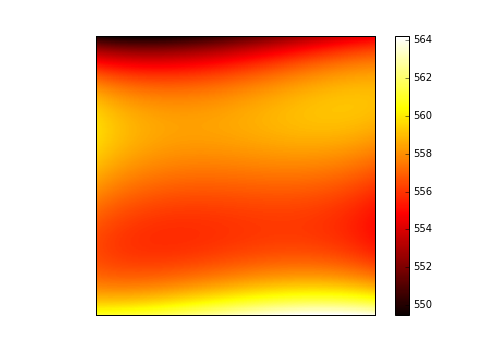
\includegraphics[scale=0.6]{figures/bkgdetail}
\caption{The background fit.}
\label{fig:bkgdetail}
\end{figure}

\section{Training a Real/Bogus Classifier Agent} \label{section:realbogus}

The subtraction techniques are very effective at  modeling PSF differences, nevertheless there are many defects left behind after a subtraction. 
This is also a well known issue in the difference image analysis. 
The bogus residual sources arise primarily from PSF mismatch and misalignments of the images.
Several simulated examples of this kind are shown in figure \ref{fig:subtraction_errors}

\begin{figure}
\centering
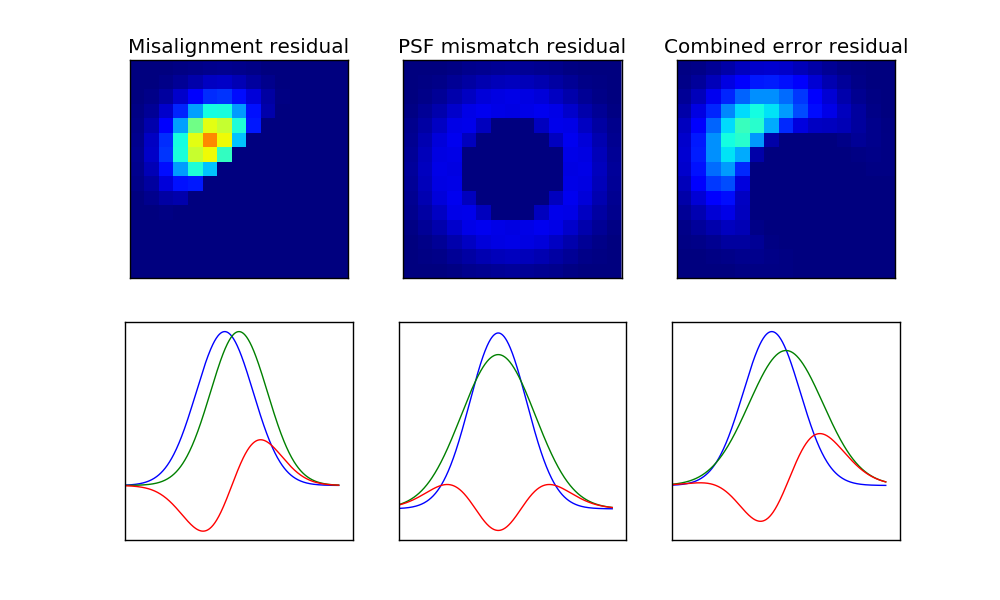
\includegraphics[scale=0.4]{figures/subtraction_error}
\caption{Some examples of subtraction errors due to misalignment and wrong PSF matching for an idealized object with a Gaussian profile.
The top row shows typical morphology of residuals for different types of mismatches.
The bottom row shows cross sections of the top row showing the object profiles in blue and green and the subtraction in red.
First column corresponds to a displacement of the object with respect to the reference. 
The second column represents objects with different PSF.
The third column is the more typical kind of bogus residual, a combination of displacement and PSF mismatch.}
\label{fig:subtraction_errors}
\end{figure}

These defects can easily confuse algorithms of source detection like SExtractor (\citet{1996A&AS..117..393B}) or similar, that relies on excess of flux over the background.
For that, it is needed to have a computerized agent capable of discriminating bogus sources from real transients on the subtracted image. 

This is the task for a Machine Learning (ML) agent. 
Machine Learning in its \emph{supervised} variant, is the general name given to a set of algorithms that can 
figure out (or ``learn'') how to classify instances by generalizing from given examples.
To be able to generalize over the given examples, a classifier must rely on some knowledge or assumptions beyond the given data.
This is referred as ``Bias''. A classifier with a large bias is very restrictive about what kind of decisions it can make on its own hypothesis space.
On the upside, this usually makes the classification robust to a new set of examples. 
That is, the efficiency of the classification has little ``Variance'' over different sets of examples.

The inverse situation is also true, classifiers with little ``Bias'' (large freedom when choosing decision boundaries) 
have big ``Variance'' of efficiency on different data sets. 
Little bias leads to the overfit of noisy features of the training examples that are not typical of larger sample sets.
For example, fitting 10 noisy points with a 10 degree polynomial has very little bias but huge variance.
On the other hand, a linear fit to the same points has a large bias, but it may well have very little variance for different sets of similar example points.
The moral is that a good classifier must have a good balance between Bias and Variance.

Machine Learning is such an extensive and intensive area of research.
It is used in web search, spam filters, recommender systems, ad placement, credit scoring, fraud detection, stock trading, drug design and many others.
Because the field is so wide, to conduct a ML experiment one must first make a few decisions. 
Even most importantly than the particular algorithm, 
for which there are hundreds, and even more are being published all the time, it's the data that drives the efficiency of the method.

%\begin{quotation}
%\em
%As a rule of thumb, a dumb algorithm with lots and lots of data beats a clever one with modest amounts of it.
%\par\raggedleft--- \textup{Lewis Carroll}, Alice in Wonderland.
%\end{quotation}

This is especially true if you want to beat the ``curse of dimensionality''.
Since your example data should sample ample portions of the feature space you are using to classify,
more data means more exploratory and generalization power.
It is generally true that a dumb algorithm with lots of data beats a clever one with modest amounts of it.

Despite the great diversity of the many ML algorithms available,
most of them are in essence a fit of a boundary decision on some feature space. 
The boundary can be very sophisticatedly constructed, but they will perform marginally better 
than a rougher simpler boundary if the data classes are well separated to begin with.
Contrary to what one would expect, the choice of the ML algorithm is not crucial in obtaining a good classification.
The main actors for a good performance in ML classification is the amount and quality of data and the feature selection.

For our main test, I decide to train a Random Forest ML algorithm on a training set developed especially for this.
The real bogus classifier, as it is referred to in the literature (\citet{2012PASP..124.1175B}),
relies on --mostly morphological-- features to perform the discrimination between ``real'' and ``bogus'' transients.

The Random Forest algorithm is an `ensemble' method.
Ensemble methods collect several other methods and put them to vote on the class. 
The final classification is given by the combined votes for each classifier.
This has the advantage of reducing the variance while only slightly increasing the bias due to combined bias of each model.
Most of the time, the decrease in variance vastly compensates for the increase in bias, yielding an overall better classification.

In this case, a Random Forest is an `ensemble' of Decision Trees. 
A Decision Tree is basically a tree of nodes. 
Each node represent a bifurcation based on one feature. 
The features and branching threshold on each node are chosen maximizing the expected information gain (or entropy loss) on the training set. 
That is, how well the bifurcation separates the training data for each class.

Random Forest bootstraps the data so that each subset of data will train a Decision Tree on a random subset of the features. 
After all Decision Trees are trained this way, the collection of Trees will give the final classification.

A single Decision Tree suffers of great variance, even for big amounts of data. 
The bifurcations on the greedy algorithm are naturally very dependent on the training set. 
A small variation on it may create a complete different tree. 
Random Forest reduces this variance by averaging over many trees. 
This also creates more realistic and fuzzy class boundaries on the feature space.

On the next section I explain how the training data was prepared.

\subsection{The Training Data and the Classifier}

The main challenge to generate training data is the great unbalance between bogus sources due to imperfect subtraction and actual real transients.

On a typical image, the number of bogus sources can be about a hundred, and the rate of real transients are usually $\lesssim$ 5. 
The Machine Learning problem becomes one of `Information Retrieval'. 
We are mainly interested in only one class, the real transients, and we need to retrieve samples of that class from a sea of bogus transients.

In such an uneven situation, a very unbalanced training set can create spurious results. As an example, imagine a training set with 90 bogus and 10 reals. 
The very naive and simple Zero Rule Classifier --that is the classifier that classifies everything as bogus-- would have a very misleading 90\% accuracy.
% 90\% Precision and 100\% Recall for the bogus class. 
An unbalanced training set could also create classifiers with large variance due to the small set of real samples.

`Recall' measures the fraction of samples of the relevant class that were retrieved by the classifier out of the total number of reals in the set.
The class we are mainly interested in for the Recall is that of the real transient examples.

To generate a balanced training set with comparable amounts of reals and bogus, I generate reals by selecting sources on an image and erasing them on the reference. 
That way, after a subtraction, those sources will pop up in the subtraction as transient events, that is, objects in the image that don't have a corresponding object on the reference.

The advantage of this method, compared to other methods like injecting fake sources, is that the `transients' obtained this way will have all the particular characteristics of the CCD and instrument from the image set in which we are interested to work. It will also have the characteristics of the subtraction method imperfections, but this is not exclusive to this method.

The `bogus' set is also collected at the same time along with the `real' set.

To have equal representation of sources of different magnitudes, the sources we use to fake the real transients are first binned into 10 bins of flux
and we pick about the same number of them from each flux bin.
We do a similar partition for the regions of the CCD. We partition the image in a 4 by 4 grid and choose equal number of sources for each portion of the CCD.
One image can be used to generate about a hundred synthetic `real' examples, and the same amount of bogus from subtraction artifacts.

We generated a training set with 7,624 examples of fabricated transients and 7,624 bogus. 
This totals 15,248 samples for training and validation.

The features used for this classifier were selected from some of the parameters available in the source extractor software SExtractor. 
We chose those features that had relation to the morphology of the source. We also constructed new features from those.
The whole list of features is presented in table \ref{mlfeatures}.

\begin{table}
\centering
\begin{tabular}{|l| >{\itshape}l|}
  \hline
  x2 & Sum of the x squared values $\sum x^2 $ \\ \hline
  y2 & Sum of the y squared values $\sum y^2 $\\ \hline
  xy & Sum of the product of x and y values $\sum xy $\\ \hline
  cxx, cyy, cxy & Same as x2, y2 and xy in the convolved image  \\ \hline
  a, b, theta & semi-major axis, semi-minor axis and orientation of the best ellipse fit to the object \\ \hline
  mag\_aper & Aperture magnitude of the object in the subtraction image \\ \hline     magerr\_aper & Error of mag\_aper \\ \hline
  flux\_aper & Aperture flux in counts of the object in the subtraction image \\ \hline
  fluxerr\_aper & Error of flux\_aper \\ \hline
%threshold & \\ \hline
flux\_max & Maximum value of the flux \\ \hline
fwhm & Full width at half maximum \\ \hline
deltax & Width in pixels of the object (X\_MAX - X\_MIN) \\ \hline
deltay & Height in pixels of the object (Y\_MAX - Y\_MIN) \\ \hline
ratio & $\min$(deltax, deltay)/ $\max$(deltax,deltay,1) \\ \hline
roundness & a/b\\ \hline
peak\_centroid & Distance in pixels from the pixel with highest count to the centroid of the object \\ \hline
\end{tabular}
\caption{Random Forest Features}
\label{mlfeatures}
\end{table}

The performance of the Random Forest classifier was determined by several efficiency parameters or `scores'.
They are all based on the Confusion Matrix, which lists the number of correct and incorrect classifications for each class.
I briefly describe each score definition below:

\begin{description}
\item[Confusion Matrix:] A square matrix the size of the number of classes whose $(i, j)$ element represents the number of classifications of the class $i$ that were classified as class $j$.\\
The diagonal has the True Positive and True Negative classifications, and the misclassifications lie on the off diagonal elements (the False Positive and False Negative cases).
A completely diagonal matrix represents a perfect classifier. \\
When the numbers are represented as proportions, they are an estimate for the True Positive Rate, the False Positive Rate, etc. In that case, it is sometimes called a ``contingency table''. \\
Confusion Matrix = $
\begin{bmatrix}
TP & FN \\ 
FP & TN
\end{bmatrix}
$ where $TP$ is true positive, $FP$ is false positive, $FN$ is false negative and $TN$ is true negative. The total number of instances is $N=TP+TN+FP+FN$. 
\item[Accuracy:] The proportion of true results (both true positives and true negatives) among the total number of classifications.
This score does not emphasize one class over the other. ($A = (TP+TN)/N$)
\item[Precision:] Precision is used when we are interested in one particular positive class (the `reals') over the other. 
Precision is then the fraction of retrieved instances that are positive.
Retrieved instances are those classified as `real', regardless of their true class. The fraction of those that are actually `real' is the \emph{precision}. \\
$P = TP/(TP+FP)$
\item[Recall:] The fraction of relevant instances that are retrieved. \\
Like with precision, it is the fraction of the total number of `reals' that were actually retrieved.\\
$R = TP/(TP + FN)$
\item[F-measure:]  Like precision and recall, the F-measure or F1, is often used in the field of information retrieval when we have one positive class. 
F-measures do not take the true negatives into account, but it combines the precision and recall into a single performance score between 0 and 1 (1 being a perfect classifier).\\
$F = 2 (P\times R)/(P + R)$
\item[Receiver Operating Characteristic (ROC) Curve:] A graph of the true positive rate against the false positive rate for different values of the discriminating threshold of the classifier.
\end{description}

Several scores of the performance of the classifier on the training data are condensed in the scores table (\ref{mlscores}).

\begin{table}
\centering
\begin{tabular}{| >{\itshape}l | l |}
  \hline
  Accuracy & 0.9935 \\ \hline
  Precision & 0.9956 \\ \hline
  Recall & 0.9915 \\ \hline
  F-measure & 0.9936 \\ \hline
  Confusion Matrix & \begin{tabular}{ l|c|c| }
\multicolumn{1}{r}{}
 &  \multicolumn{1}{c}{real}
 & \multicolumn{1}{c}{bogus} \\
\cline{2-3}
{\it Classified as} real & 7591 & 33 \\
\cline{2-3}
{\it Classified as} bogus & 65 & 7559 \\
\cline{2-3}
\end{tabular} \\ \hline
\end{tabular}
\caption{Random Forest Scores}
\label{mlscores}
\end{table}

On the training data, the performance is quite good, with all indicators scoring above 99 percent.

In the confusion matrix we see that only 65 out of 7,624 of the reals were mis-classified as bogus, and only 33 bogus out of the 7,624 were mis-classified as reals. These very low numbers explain the very high performance scores of the classifier.

Random Forest can also provide an importance score based on how up in the tree structure it is within a tree.
The features with most discriminative power are selected as first decision nodes.
In figure \ref{fig:featureimportance} we show a graph listing the importance for each of the features along with one standard deviation.
The importance was calculated with a single Random Forest classifier with 10,000 trees and a maximum depth of 10.
We can see that the first 10 or so features carry the most information, but except for the flux, most of them are equally important.
We can also see that we could drop the last 4 (delta\_x, delta\_y, ratio and threshold) without significantly affecting the overall performance.

\begin{figure}
\centering
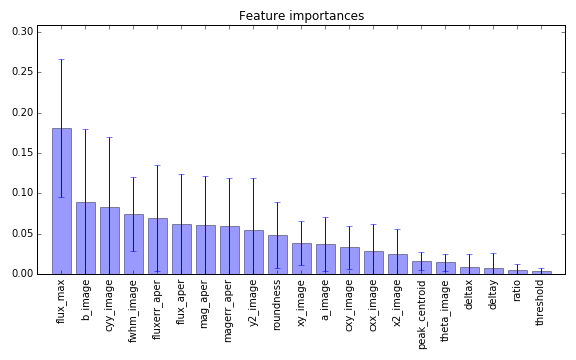
\includegraphics[scale=0.6]{figures/featureimportance}
\caption{The relative `importance' of each feature calculated with Random Forest algorithm.}
\label{fig:featureimportance}
\end{figure}

In figure \ref{fig:rbfeathist} we can see the histograms for the real population and the bogus populations separated, for the 4 most 
important features given by the Random Forest fit.
We can see that none of the features by itself clearly separates the data, as it is usually the case for typical features.

\begin{figure}
\centering
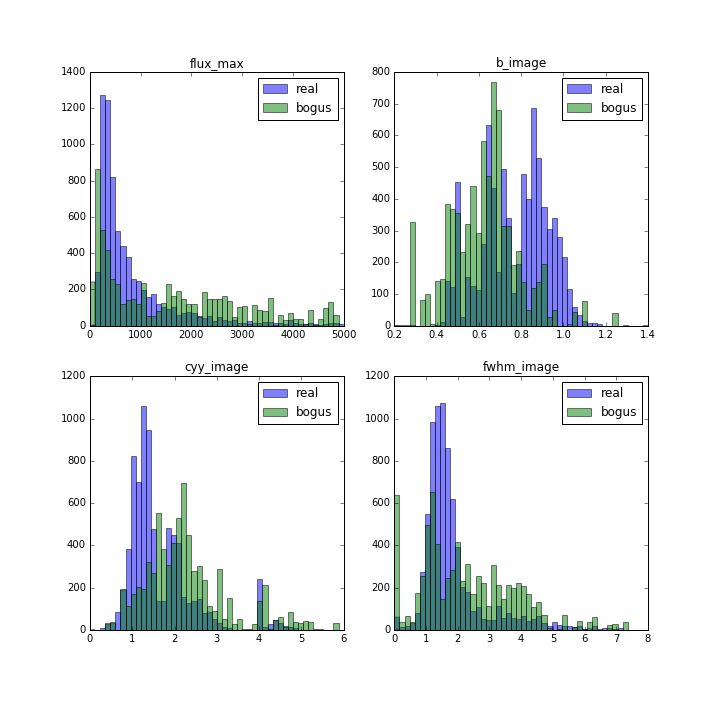
\includegraphics[scale=0.6]{figures/hist_rbfeatures}
\caption{Histograms for the 4 most important features as given by the Random Forest fit, separated by the real and bogus population.}
\label{fig:rbfeathist}
\end{figure}

\begin{comment}
\subsection{Testing the classifier on real data}

Once we have trained our classifier with training data, we wanted to also test it in a more real situation. For that we apply the classifier to the rest of the cstar\_june\_selection data set in search of actual transients of the image.

The Random Forest classifier will not only predict the class, but can also output a probability for that class.

Setting the probability to 0.9, the classifier returns the most likely transient events. The rate of real transient in the images is of about 15 per image for this probability threshold.

Some examples of these are shown in figure ??.

For very faint events or events that comprise very few pixels in the image, we can have additional filters that weed them out. Although, some of this could be of astronomical interest and discarding them could result in its loss.
\end{comment}

\section{Results}

We created a pipeline that is capable of responding to detection alerts sent by LVC.
The set of processes that trigger the alert are condensed into a script running on one of the University of Texas Rio Grande Valley servers.
The script parses the VOEvent alert file, capturing metadata of the detection, downloads the skymaps for the localization uncertainty
and creates targets for the telescopes, based on criteria of potential host galaxy, visibility at the time of the event and probability of hosting the event.

The mock run on CSTAR data showed that the differential photometry analysis together with a Real-Bogus ML classifier trained on the same data set 
can be used to select possible candidates of counterpart transients.

The Real-Bogus classifier achieved scores above 99\% on validation sets of synthetic examples that we generated.

Incidentally, we also tested the alignment routines to stack images for subtraction, and several types of different Optimal Subtraction algorithms.


%%%%%%%%%%%%%%%%%%%%%%%%%%%%%%%%%%%%%%%%%%%%%%%%%%%%%%%%%
%
%			O1 Observations
%
%%%%%%%%%%%%%%%%%%%%%%%%%%%%%%%%%%%%%%%%%%%%%%%%%%%%%%%%%
\chapter{Observations for GW150914 Optical Counterparts}

\emph{Note: Part the work described in this chapter has been previously published in a 2016 paper with the title 
``GW150914: First search for the electromagnetic counterpart of a gravitational-wave event by the TOROS collaboration''
in {\it The Astrophysical Journal Letters}, Volume 828, Issue 2, article id. L16, 6 pp. 
The authors of this publication are Mario C. Diaz, Martin Beroiz, Tania Penuela, Lucas M. Macri, Ryan J. Oelkers, 
Diego Garcia Lambas, Juan Cabral, Carlos Colazo, Mariano Dominguez, Bruno Sanchez, Sebastian Gurovich,
Marcelo Lares, Dario Grana, Victor Renzi, Horacio Rodriguez, Manuel Starck, Ruben Vrech, Rodolfo Artola, 
Antonio Chiavassa Ferreyra, Carla Girardini, Cecilia Quinones, Luis Tapia, Marina Tornatore, Jennifer L. Marshall,
Darren L. DePoy, Marica Branchesi, Enzo Brocato, Nelson Padilla, Nicolas A. Pereyra, Soma Mukherjee, Matthew Benacquista and Joey Key.
}

On April 2014, TOROS signed a Memorandum Of Understanding (MOU) with the LIGO Virgo Collaboration, in order to participate 
in a program to perform follow-up observations of GW candidate events with the benefit of access to LVC proprietary information.

The MOU signing was a very important step that allowed TOROS to participate in the O1 LIGO campaign with positive results.
The MOU allowed TOROS to receive the LIGO alerts, which were private and confidential at the time of O1, 
and to be part of a publication as part of a broader collaboration with other institutions for the electromagnetic counterpart search of the first announced GW ever, namely GW150914.

The O1 campaign was a 4 month run, officially started on September 18, 2015 and ended on January 12, 2016.
Two detectors were operational during the whole run, the H1-L1 network, operating with a BNS range of about 60 Mpc.
The Virgo detector was being upgraded during O1 so it was not part of the operating detectors during the run.
During O1, 3 alerts were issued for 3 different events.

The first one was from an event detected by LIGO instruments on September 14, 2015 at 09:50:45 UTC (\citet{2016PhRvL.116f1102A}).
The event was designated after confirmation, with the code GW150914.
This was also the first confirmed Binary BH merger ever detected through its gravitational waves.
TOROS observed several regions of the sky during the night that we received the alert.

GW150914 reached the LIGO instruments with a significance greater than 5.3$\sigma$
and a combined signal to noise ratio (SNR) of 23.7.
The GW signal matched with a template for a binary with primary mass of $36.2^{+5.2}_{-3.8} M_{\odot}$ 
and a secondary mass of $29.1^{+3.7}_{-4.4} M_{\odot}$.
The final mass of the system after merger $62.3^{+3.7}_{-3.1} M_{\odot}$ with a final spin $0.68^{+0.05}_{0.06}$,
that represents a total radiated energy of $3.0^{+0.5}_{-0.4} M_{\odot} c^2$.
The luminosity distance to the merger is $420^{+150}_{-180}$Mpc, or a redshift $z=0.09^{+0.03}_{-0.04}$.

The second one, LVT151012 (\citet{2016PhRvX...6d1015A}) did not cross the 5$\sigma$ significance threshold,
but, according to the authors ``it is more likely to have resulted from a gravitational-wave signal than from an instrumental or environmental noise transient'' .
LVT151012 has a significance of $1.7 \sigma$ and a combined SNR of 9.7.
If it is a result of a BBH merger, it would be a system with 23 and 13 $M_{\odot}$.

The third and last confirmed event for O1, GW151226 (\citet{2016PhRvL.116x1103A}), had a significance over $5.3 \sigma$ and a combined SNR of 13.0.
The GW signal was consistent with a template match for a binary system with masses 14.2 and 7.5 $M_{\odot}$.
The final mass of the merger is $20.8 M_{\odot}$, which means that $1 M_{\odot}$ was radiated away as gravitational radiation.

TOROS did not participate in the optical search for LVT151012 or GW151226.
The remaining of this chapter refer to the observation campaign for the GW150914 event follow-up search and its results.

\section{GW150914}

GW150914 was detected on September 14, 2015 at 09:50:45 UT (see figure \ref{fig:GW150914ligosignal}).
LIGO had not officially started the O1 campaign at that time, which was scheduled to start on September 18, 4 days later. 
It was instead at the end of the last engineering run E7.

\begin{figure}
\centering
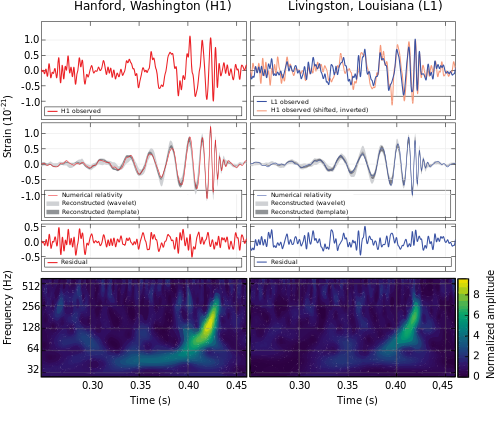
\includegraphics[scale=0.5]{figures/GW150914detection}
\caption{GW150914 event observed by the LIGO Hanford (H1, left column panels) and Livingston (L1, right column panels) detectors. 
Top row is the strain signal. Second row is the GW strain projected onto each detector in the 35--350 Hz band. 
Solid lines show a numerical relativity waveform for a system with parameters consistent with those recovered from GW150914. 
Third row: Residuals after subtracting the filtered numerical relativity waveform from the filtered detector time series. 
Bottom row: A time frequency representation of the strain data.}
\label{fig:GW150914ligosignal}
\end{figure}

Despite the premature arrival of the GW detection, LIGO sent the alert via a private GCN initial circular (Singer 2015, GCN\#18330) to the MOU partners two days later.
This unexpected detection constituted the first detection of the merger of a binary black hole (BBH) system and the first direct detection of gravitational waves. 

TOROS received the alert through the robot alert system and we began our imaging campaign immediately after receiving, on the night of of 2015 September 16. 
Additional observations were obtained the following night, and a second epoch of imaging was acquired on 2015 December 5 \& 6. 

The initial GCN alert contained a coherent Wave Burst (cWB) all sky localization map, and a subsequent update GCN notice delivered an Omicron+LALInference Burst (oLIB) skymap. 
Both skymaps are based on a search for unmodeled signals. 
The first one, a rapid localization analysis just searches for coherent power across both detectors while the second one assumes a Sine-Gaussian content. 
The maps provided initial spatial localization of 50\% and 90\% confidence regions encompassing about 200 and 750 square degrees, respectively.

The targets were selected based on the first skymap provided, the cWB localization map.

Besides the LIGO-Virgo Collaboration, other 24 institutions participated in the optical counterpart search for the GW150914 event along with TOROS.
These are detailed in table \ref{gw150914participants}.

\begin{table}
\centering
\begin{tabular}{|l|c|}
\hline
Institution name & Band \\ \hline
The LIGO Scientific Collaboration & GW \\
The Virgo Collaboration & GW \\
The Australian Square Kilometer Array Pathfinder (ASKAP) Collaboration & Radio \\
The Bootes Collaboration & Optical \\
The Dark Energy Survey And The Dark Energy Camera GW-EM Collaborations & Optical/NIR \\
The Fermi GBM Collaboration & $\gamma$-rays \\
The Fermi LAT Collaboration & $\gamma$-rays \\
The Gravitational Wave Inaf Team (Grawita) & Optical/NIR \\
The Integral Collaboration &  $\gamma$-rays \\
The Intermediate Palomar Transient Factory (iPTF) Collaboration & Optical \\
The Interplanetary Network & $\gamma$-rays \\
The J-Gem Collaboration & Optical \\
The La Silla-Quest Survey & Optical \\
The Liverpool Telescope Collaboration & Optical \\
The Low Frequency Array (LOFAR) Collaboration & Radio \\
The Master Collaboration & Optical \\
The Maxi Collaboration & X-ray \\
The Murchison Wide-field Array (MWA) Collaboration & Radio \\
The Pan-STARRS Collaboration & Optical \\
The PESSTO Collaboration & Optical \\
The Pi Of The Sky Collaboration & Optical \\
The SkyMapper Collaboration & Optical \\
The Swift Collaboration & $\gamma$-rays \\
The Tarot, Zadko, Algerian National Observatory, And C2PU Collaboration & Optical \\
The TOROS Collaboration & Optical \\
The Vista Collaboration & Optical and Infrared \\ 
\hline
\end{tabular}
\caption{Participating Institutions in the GW150914 EM Counterpart Search}
\label{gw150914participants}
\end{table}

For the observations we used the 1.5-m telescope at Estacion Astronomica Bosque Alegre (EABA) in Cordoba, Argentina (the smaller telescope at Macon was not operational at the time).
The telescope uses an Apogee Alta U9 camera with a field of view (FoV) of 12.'7 $\times$ 8.'5 and
an effective plate scale of 0.''75pix after 3 $\times$ 3 binning. 
% Tell what is the pixel width and height!
Since we wanted to maximize our sensitivity, we conducted unfiltered (``white light'') observations spanning 0.35 < $\lambda/\mu$m < 1. 
We obtained individual exposures of 60 s with a median seeing (FWHM) of (2.8 $\pm$ 0.6)''. 
We typically obtained 10 images per field, reaching 5$\sigma$ limiting magnitudes of r = 21.7 $\pm$ 0.3 mag in the AB system.

We were able to scan a small region of the LIGO localization map and contribute to the EM counterpart search, 
even though the search did not show up any transient associated with the event.
Despite the little area covered by TOROS, the O1 campaign allowed the collaboration to test the detection and response systems to the alerts.

\section{Target Selection}

The LIGO localization regions are very poorly constrained because they are based mainly on triangulation.
Confidence regions can span several hundred square degrees (see figure \ref{fig:pointings}), and they also vary depending on the algorithm. 
For instance, the 90\% credible localization area for the cWB skymap covers 310 square degrees, 
while others span up to 750 square degrees (see table 1 in \citet{2016ApJS..225....8A}). 
It greatly exceeds the fields of view of most radio, optical, and X-ray telescopes.
Regardless, all sky maps are consistent with a broad long arc in the Southern hemisphere and a smaller extension in the Northern hemisphere. 

\begin{figure}
\centering
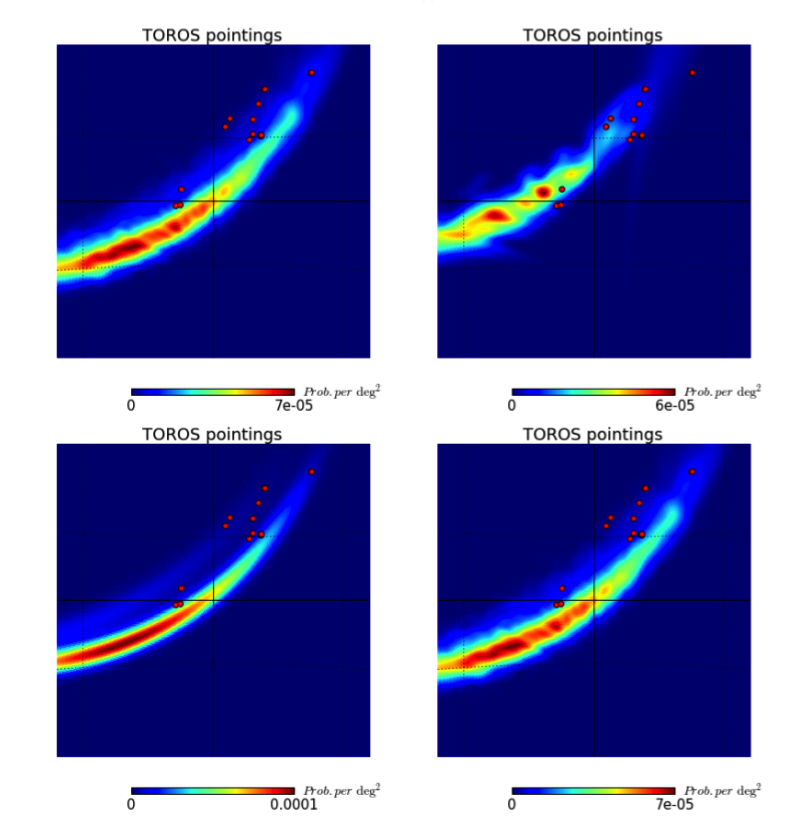
\includegraphics[scale=0.5]{figures/pointings}
\caption{cWB, LIB, BYST, LALinf Sky-maps re-scaled regions that mark TOROS targets (red dots).}
\label{fig:pointings}
\end{figure}

The algorithm utilized for the cWB estimations produces reasonably accurate maps for BBH signals, but underestimates the extent of high-confidence regions (\citet{2015ApJ...800...81E}). 
As seen in figure \ref{fig:pointings}), the adoption of maps from alternative algorithms (not available at the time our observations started) 
significantly reduced the fraction of the high-confidence region probed by our small field of view.

As the LIGO analysis was underway at the time our observations began and the nature of the binary was unknown, 
we optimized the use of our small field of view by targeting nearby galaxies with the highest probability of hosting the event.
As we described in section \ref{targetselection}, the target selection is based on two main criteria: 
the localization (un)certainty on the target pixel in the all-sky map given by LIGO at the time of the alert, 
and several filter cuts on distance, blue luminosity and apparent magnitude on the list of galaxies in the GW Galaxy Catalog (GWGC) (\citet{2011CQGra..28h5016W}).
The cut in absolute magnitude for $MB \le -21$ mag was motivated by the expectation that in the nearby Universe the distribution of BNS and BHs 
should follow recent star formation due to the short merger timescales (see e.g. \citet{1991ApJ...380L..17P, 2002ApJ...572..407B}).

The filtered galaxies are assigned individual probabilities $P_{g,i}$ (with $i$ being the sky map pixel that contained the $g$-th galaxy)
to prioritize targets according to their location within the sky maps.

Lastly, we ensured that all targets were mapped out to about 5kpc, which corresponds to the median offset distance of short GRBs 
from hosts galaxies measured from the optical afterglow observations (\citet{2011MNRAS.413.2004C, 2013ApJ...776...18F, 2014ARA&A..52...43B}).
This required tiling to cover the appropriate area for some targets. 
A total of 21 fields were observed.

This joint filters for GW and Optical parameters ensures the targets are visible at each telescope site, 
and that they have some significant probability of being the host. 
The list of filter cuts for the observations are summarized in table \ref{obsfilters}.

\begin{table}
\centering
\begin{tabular}{|l|c|}
  \hline
 Parameter & Limit value \\ \hline
Observability from location & $30^{\circ} > \delta > -70^{\circ}$ for EABA \\ \hline
Apparent Magnitude & $B \le 21$ mag \\ \hline
Distance  & $D < 60$ Mpc \\ \hline
Absolute Magnitude & $MB \le -21$ mag \\ \hline
\end{tabular}
\caption{Parameter Cuts}
\label{obsfilters}
\end{table}

The list of the galaxies that came up in the search are summarized in table \ref{o1targets}.
Galaxies PGC381152 and PGC075108 are actually contained in the same frame.
For galaxies IC1933, NGC1529 and IC2038, we tiled four frames around the galaxy to cover more area around the target. 

\begin{table}
\centering
\begin{tabular}{|*{7}{c|}}
  \hline
 Date & GWGC & RA & Dec & $t_{exp}$ & Tile & D \\ 
 (Local Time) & ID & [Deg] & [Deg] & [s] & Number & [Mpc] \\ \hline
2015-09-16 & IC1933 & 51.416101 & -52.78547 & 600 & 1,2,3,4 & 17.45 \\
2015-09-16 & NGC1529 & 61.833301 & -62.89993 & 600 & 5,6,7,8 & 54.76 \\
2015-09-16 & IC2038 & 62.225246 & -55.99074 & 600 & 9,10,11,12 & 7.00 \\
2015-09-16 & IC2039 & 62.259901 & -56.01172 & 600 & 9,10,11,12 & 7.63 \\
2015-09-17 & ESO058-018 & 102.593850 & -71.03123 & 1020 & 13 & 52.23 \\
2015-09-17 & ESO084-015 & 65.550449 & -63.61097 & 1140 & 14 & 14.99 \\
2015-09-17 & ESO119-005 & 72.072451 & -60.29376 & 1080 & 15 & 9.73 \\
2015-09-17 & NGC1559 & 64.398901 & -62.78358 & 900 & 16 & 12.59 \\
2015-09-17 & PGC016318 & 73.728898 & -61.56747 & 1020 & 17 & 9.54 \\
2015-09-17 & PGC269445 & 100.209150 & -71.33026 & 1140 & 18 & 54.83 \\
2015-09-17 & PGC280995 & 96.382499 & -69.15257 & 1140 & 19 & 55.08 \\
2015-09-17 & PGC128075 & 64.859998 & -60.53844 & 720 & 20 & 63.71 \\
2015-09-17 & PGC381152 & 63.584547 & -58.20726 & 1200 & 21 & 13.26 \\
2015-09-17 & PGC075108 & 63.670349 & -58.13199 & 1200 & 21 & 13.29 \\ \hline
\end{tabular}
\caption{Targeted host galaxies}
\label{o1targets}
\end{table}


%Maybe add the probability at the center of the galaxy?

%We show some of the target frames in figure \ref{}.


\section{Image Preprocessing}

The first step for processing the images is to prepare the bias and flat frames.

The bias frame is generated by reading the CCD with no exposure time (immediate read-out of 0 seconds exposure).
When a CCD is read out, not all the pixels start out at a value of zero, because of the intrinsic CCD read noise.
The bias frame needs to be subtracted from the image to bring all the pixels to an equal starting value.
We used a median stack of XX bias frames taken the night of the observation. \textcolor{red}{complete using details}

The flat frame is an image with (ideally) the same exposure time as the images we need to preprocess, illuminated as uniformly as possible.
Flat frames correct for dirt or dust in the telescope system, vignetting and internal reflections.
Telescopes use either a ``dome flat'', which is typically images of a white screen installed on the dome of the telescope or ``sky flats'' which are images of the twilight sky.
The observations for GW150914 had all dome flats, as well as most of the images taken for the a posteriori references, except for a few reference tiles that had a sky flat.
Just like in the case of bias frames, flat frames are coadded using the median. \textcolor{red}{complete using details}

Once we have a good bias and flat frame, we combine them with the light frames (target images) as per the following equation:

\begin{equation}
S = \frac{L - B}{F - B}
\end{equation}

where $S$ is the final science image, $L$ is the light frame, $B$ is the bias frame and $F$ is the flat frame.

The registration of the image on the World Coordinate System (WCS) with at TAN/SIP proection, 
was done with the program astrometry.net (\citet{2010AJ....139.1782L}).

The CCD we used to take the images contained several dead pixels and bad columns that needed to be masked.
To identify the bad pixels on the CCD, we stacked all of the bias frames and applied a threshold cut on the pixel value, 
to identify those pixels with little to null response to light exposure.
We then increased the bad pixel mask to 1 pixel in each direction to make sure any residual near the bad column or pixel is not identified as a real variation.
A mask FITS file was created and propagated along through each of the following steps (registration, stacking and image differencing).

The next step was to create median stacking of the science images to improve SNR and removing cosmic rays and artifacts.
After a visual inspection, we excluded some frames because they had visible motion blur, or were affected by partial cloud coverage.
This resulted in some tiles having shorter effective exposure time (see table \ref{o1targets}).
During the stacking of the science images, we replaced the bad pixels with noise consistent with the normal background distribution on the image.
Finally, we used circular masks to cover saturated stars on the frames. 

The same procedure was done on the \emph{a posteriori} reference frames.
The reference images were taken a few months after the alert, on 2015 December 5 \& 6, using the same telescope in Bosque Alegre.
They were taken with the same exposure time for all fields and the same binning.

The final step is to align the reference to the science images to perform the image subtraction.
We aligned the images using the Python module astroalign, which matches 3-star asterisms on both images to find the optimal affine transformation between the two frames. 
It then performs a bi-cubic interpolation of the image to do the alignment (see section \ref{section:astroalign} for more details).
For this work, we avoided the rotations, since they were all smaller than $10^{-7}$ rad, to prevent the creation of more bogus transients during the subtraction.

We propagated the headers through all the steps and created a new WCS for the aligned image.


\section{Difference Imaging Analysis}

To search for potential transients on the images taken we performed a differential photometry analysis on them.

Our method follows the work of \citet{2008MNRAS.386L..77B} and \citet{2008PASP..120..449M} in a Python implementation of the 
algorithms (see section \ref{section:ois} for more details).

As explained in section \ref{section:dia}, the Bramich method uses the information from all the pixels on the image, wether is part of the background or a source,
so we don't need to select specific stars to take stamps around.
We partitioned the images in a 2$\times$3 grid to compensate for possible PSF variability across the field of view.
Even though the Python \emph{ois} module can do a simultaneous background estimation to be subtracted, 
we noticed that for images with large extended objects on the image, like tile \#16 for NGC1559, 
the background was introducing large depressions of negative pixels and we had to turn background estimation on those.

\section{Real-Bogus classification and detection of potential transients}

To inspect for the possibility of transients on the science images we perform a Real/Bogus search on the difference images, 
as we did with the CSTAR image set in section \ref{section:realbogus}.
We erase stars on the reference images to create fictitious transients after a subtraction is made.
We perform the subtraction using the Python module \emph{ois} (see section \ref{section:ois}).

Once the subtraction is done, we run SExtractor on the subtraction to recover these fabricated transients and their associated SExtractor parameters.
One difference with the procedure done with CSTAR is that we do not separate sources into flux bins, because we have relatively much fewer stars in the field.

For each transient we generate this way we add an equal amount of subtraction bogus artifact, to keep the training set balanced in number.
We worked with 1511 examples of `real' transients and 1511 examples of `bogus' subtraction artifacts
taken from tiles 13, 14, 16, 17, 18, 19 and 20 (see table \ref{o1targets}).
With these we trained a classifier.

The classifier had very good score statistics, but not as good as the one with CSTAR, most likely because of the lower sampling of `transient' examples.
Nonetheless all performance statistics score above 90\%.

The particular Random Forest algorithm we used is the one provided in \emph{scikit-learn} (\citet{2012arXiv1201.0490P}), a popular Python package for Machine Learning analysis.
We have 10 Decision Trees in the ensemble, each one with a `Gini impurity' criterion to decide on the split of the branches.
Each tree decides based on the square root of the number of features. On our case, with the features in table \ref{mlfeatures}, 
the algorithm will branch its decisions based on 4 features randomly chosen.

% self, n_estimators=10, criterion='gini', max_depth=None, min_samples_split=2, min_samples_leaf=1, min_weight_fraction_leaf=0.0, max_features='auto', max_leaf_nodes=None, min_impurity_split=1e-07, bootstrap=True, oob_score=False, n_jobs=1, random_state=None, verbose=0, warm_start=False, class_weight=None

Several scores of the training are given on table \ref{gwscores} including the confusion matrix of the training.
The receiver operating characteristic (ROC) curve is presented in figure \ref{fig:roc_gw150914}.

\begin{comment}
\begin{table}
\centering
\begin{tabular}{ l|c|c| }
\multicolumn{1}{r}{}
 &  \multicolumn{1}{c}{real}
 & \multicolumn{1}{c}{bogus} \\
\cline{2-3}
{\it Classified as} real & 1390 & 121 \\
\cline{2-3}
{\it Classified as} bogus & 144 & 1367 \\
\cline{2-3}
\end{tabular}
\caption{Confusion Matrix}
\label{gwconfusionmatrix}
\end{table}
\end{comment}

\begin{table}
\centering
\begin{tabular}{| >{\itshape}l | l |}
  \hline
  accuracy & 0.9123 \\ \hline
  precision & 0.9186 \\ \hline
  recall & 0.9046 \\ \hline
  F measure & 0.9116 \\ \hline
  Confusion Matrix & \begin{tabular}{ l|c|c| }
\multicolumn{1}{r}{}
 &  \multicolumn{1}{c}{real}
 & \multicolumn{1}{c}{bogus} \\
\cline{2-3}
{\it Classified as} real & 1390 & 121 \\
\cline{2-3}
{\it Classified as} bogus & 144 & 1367 \\
\cline{2-3}
\end{tabular} \\ \hline
\end{tabular}
\caption{Random Forest Scores}
\label{gwscores}
\end{table}

Applying this Real-Bogus classifier on subtraction images for that day, resulted in zero potential transient candidates in all images 
with probability of being real over 90\%, and only 40 above 80\%.
There were 226 potential candidates with probability over 50\%.
As a final discrimination against spurious detections, we required an object to be detected in at least 5 of 10 realizations
of a given field in order to be considered a bona fide astrophysical transient. 
None of the objects in either set passed this requirement. 
Further visual inspection revealed most of them to be subtraction residuals or cosmetic defects in the detector. 
We therefore conclude that no transients were present in the 21 fields we targeted, to a 5$\sigma$ limiting magnitude of r = 21.7 in the AB system.

\begin{figure}
\centering
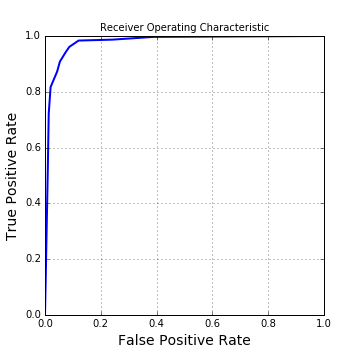
\includegraphics[scale=0.6]{figures/roc_gw150914}
\caption{The ROC curve for the Random Forest classifier trained with transients generated from the images.}
\label{fig:roc_gw150914}
\end{figure}


\section{Results}
The TOROS collaboration conducted a prompt search for the electromagnetic counterpart of the 
first gravitational-wave event reported by LIGO using the 1.5-m telescope of Estacion Astrofisica Bosque Alegre (EABA) in Cordoba, Argentina. 

Our search spanned two nights, during which we targeted 14 targets in 21 fields containing nearby (D < 60 Mpc) luminous (MB <  21 mag) 
galaxies with high probabilities of hosting the event. 
We covered 0.62 square degrees which corresponds to an integrated probability of about 0.03\% in the cWB map and less than 0.01\% in the rest of the skymaps.
We reached a 5$\sigma$ limiting AB magnitude of r = 21.7.

The fact that we did not find any genuine transient in our search is not surprising given the small area surveyed (\textasciitilde 0.62 sq. degrees) 
and the low cadence of the observations (with only two epochs per target, separated by 73$\pm$3d). 
The fact that we did not find any genuine transient in our search is not surprising given the small area surveyed (\textasciitilde{}0.62 sq. degrees) 
and the low cadence of the observations (with only two epochs per target, separated by 73$\pm$3d). 

Based on our temporal sampling and photometric precision, we scaled the results of \citet{2015AJ....149...50O} 
to estimate that only 1 in \textasciitilde{}3,030 stars in our fields would exhibit variability detectable at the 5$\sigma$ level over this timescale. 

Given that only 4,200 stars were detected across all fields by DAOPHOT, we would only expect to detect \textasciitilde1 variable star.
Regarding extragalactic transients, based on supernova Ia rate for R < 21 mag of 10 events per square degree per year
(\citet{1996ApJ...473..356P, 2004IBVS.5519....1G}) and a 30\% fraction of SN Ia among local SNe (\citet{2016ApJ...822...48G}), 
we estimate an 11\% probability of finding such an object across all our fields. 
Finally, our result is consistent with the LIGO detection of a binary black hole merger, for which no optical EM counterpart is expected.

No bona fide events were found, a result that is consistent with the low probability of detecting stellar or extragalactic variability 
given our temporal and areal coverage, and with the later classification of the GW event as a merger of two stellar-mass black holes.



%%%%%%%%%%%%%%%%%%%%%%%%%%%%%%%%%%%%%%%%%%%%%%%%%%%%%%%%%
%
%			Software
%
%%%%%%%%%%%%%%%%%%%%%%%%%%%%%%%%%%%%%%%%%%%%%%%%%%%%%%%%%


\chapter{Software Developed}

The first attempts to build software for the TOROS pipeline lacked modularity, or in the language of Computer Science, \emph{separation of concerns}.
Separation of concerns (SoC) is a design principle in Computer Science for separating a computer program into distinct sections,
such that each section addresses a separate concern. 
In our pipeline we had many different areas of concern: the alert system; the image preprocessing; the alignment of images; and the differential photometry of the subtractions.
As the code matured, each area of concerned became naturally separated from the main trunk of development, which was at the moment rather monolithic in nature. 

The Python way to address SoC is through the use of modules and packages, so this separation naturally led to the creation of Python modules of more general use, 
that were later integrated back into the pipeline as external imports.

As is well known, modularity is achieved by encapsulating information inside a section of code that has a well-defined interface.
Having well-separated concerns ensures that each part can be reused and also helps in the maintenance and updating of the code.

The modules are released under MIT License and are hosted on a organization repository in the popular Git repository hosting service, 
github\footnote{\url{https://github.com/toros-astro/}}.
Two of them have unit tests and hooked to travis-ci website for continuous-integration and code coverage.

In the following sections I describe some of the Python modules we developed in more detail.

\section{Astroalign }\label{section:astroalign}

Astroalign was developed to address the need to align two images before subtraction.
There are currently two other Python modules with similar functionality.
The module \emph{reproject} will resample or reproject images when WCS information is provided, but it does not address the problem of registration when one or both images lack WCS information.
The module \emph{alipy} does not rely on WCS information, but uses external programs like IRAF and SExtractor and deals exclusively in the FITS format for images.
Astroalign works with the raw pixel information in memory, so it's agnostic about the source of the images.
It is also self contained, so does not rely on any external program to perform the alignment
and it is written entirely in Python.

Astroalign is inspired by the method of the C program astrometry.net (citet{2010AJ....139.1782L}).

Astrometry.net's goal is much more ambitious than our present problem of aligning two images.
Their program's main goal is to identify the portion of the sky that an image belongs to, and it solves this problem remarkably well.
It will also generate WCS header information along with other details like pixel scale and orientation.
The process can take several minutes to complete and requires downloading a few invariant databases for the specific case we need.

Astrometry.net uses 4-star asterisms (or quadrilaterals) from the image,
to match them against a previously-created huge database of asterisms from catalogs of stars of the whole sky.
The efficiency of astrometry.net is on the power of this database of cataloged stars.

For \emph{astroalign}, we don't need a catalog of the whole sky, since we are only interested in the region of the sky covered by the image at hand. 
We can create a catalog of the region of interest, using the reference frame.
In essence we will have a catalog of some bright reference stars on each image, 
and we want to match them in some way to find the appropriate affine transformation between the images.

As we mentioned before, the core idea of the algorithm consists on characterizing asterisms on the image in a unique way, 
by using quantities invariant to translation, rotation or even scaling and flipping.
For astroalign, I use 3-star asterisms (or triangles) to perform the matching, and a RANSAC algorithm to decide on the final transformation.
Similar asterisms will have the same invariant tuples in both images so a correspondence can be made between those invariant quantities. In a way, this invariants are proxies or unique ID's for the asterisms.

The lengths of the sides of a triangle are invariant to translation and rotation, they remain the same whatever position or orientation the triangle may have, but are not invariant to scaling.
If we want to fully characterize a triangle up to a global scaling, then knowing 2 inner angles is enough. 
Equivalently, knowing 2 independent ratios of the side lengths is also sufficient.
In fact any function of 2 independent length ratios will also do.

For astroalign, we used the following simple invariants.

\begin{align*}
I(L_i,L_j,L_k) =& \left( \frac{L_2}{L_1}, \frac{L_1}{L_0} \right) = (I_{1}, I_{2}) \numberthis \label{invdef} \\ 
 & \text{where} \left\{
  \begin{array}{lll} 
 L_2 &=& \max\{L_{i}\}_{i=1,2,3} \\
 L_1&=&\text{middle}\{ L_{i} \}_{i=1,2,3} \\ 
 L_0 &=& \min\{ L _{i} \}_{i=1,2,3}
  \end{array}
\right.
\end{align*}

The idea for the astroalign algorithm can be summarized in a few steps

\begin{enumerate}
\item Do for both images \begin{enumerate}
\item Make a catalog of a few brightest sources (but not too few!)
\item Push these sources into a 2d-tree to quickly query for close neighbors\footnote{A kd-tree data structure for k=2 retrieves nearest neighbors in $\mathcal{O}(N \log N)$ number of operations on average.}.
\item For each star, select the 4 nearest neighbors (5 sources including the star itself).
\item Form all the ${5}\choose{3}$ possible triangles from that set of stars.
\item For each triangle in that set, calculate the tuple of invariants in \ref{invdef}, that uniquely identify the triangle and push the invariant tuple into another kd-tree.
\item There could be many duplicate triangles on the previous list, so it's best to remove them leaving only unique elements.
\end{enumerate}
\item Do with RANSAC \begin{enumerate}
	\item For a randomly chosen invariant in the image, find a corresponding (if any) invariant on the reference kd-tree.
	\item As long as the triangle is not equilateral, one can further make a correspondence of individual stars within a triangle pair, by looking at which side of the triangle they belong.
	This way, one can make a star to star identification on both images, and have a candidate transformation matrix based on this triangle match.
	\item The transformation is considered satisfactory is it can match at least 80\% of the other stars in the catalog.
	If it is not satisfactory, iterate RANSAC until one affine transformation is found, or until we reach the maximum number of iterations.
\end{enumerate}
\end{enumerate}

Astroalign needs reference stars to work with and for that reason it is not suitable for images of extended objects with no visible stars.
On the opposite situation, it will also struggle in very crowded fields like globular clusters because of the large quantity of similarly bright stars.
Astroalign's optimal use is in stellar images where stars are relatively isolated from their neighbors.


\subsection{Analysis of the Asterism Invariants}

Let's analyze here the invariant set \ref{invdef} given in the previous section.

This choice of invariants maps the positive octant of $\mathbb{R}^3$ of all possible side lengths of a triangle, 
onto a region of the positive quadrant of $\mathbb{R}^2$ in the invariant-features space.

To find out what this region is, we notice that since $L_2 > L_1 > L_0$,

\begin{align*}
x &=  \frac{L_2}{L_1} > 1 \\
y &=  \frac{L_1}{L_0} > 1
\end{align*}

Also, using the triangle inequality:

\begin{align*}
L_2 \leq L_1 + L_0 \implies & x \leq 1 + \frac{1}{y} \\
& y \leq \frac{1}{x-1}
\end{align*}

The curve $y = (x-1)^{-1}$ corresponds to co-linear points.

Also, it's worth noting that any equilateral triangle will map to the point $(1,1)$; 
and an isosceles triangle will map to either the $x=1$ or $y=1$ line, depending on whether the unequal side is the longest or the shortest.

Very peaky triangles will tend to accumulate between the co-linear points curve and the $x=1$ line for large values of $y$.

All these observations can be summarized in figure \ref{fig:inv_region}.

\begin{figure}
   \centering
   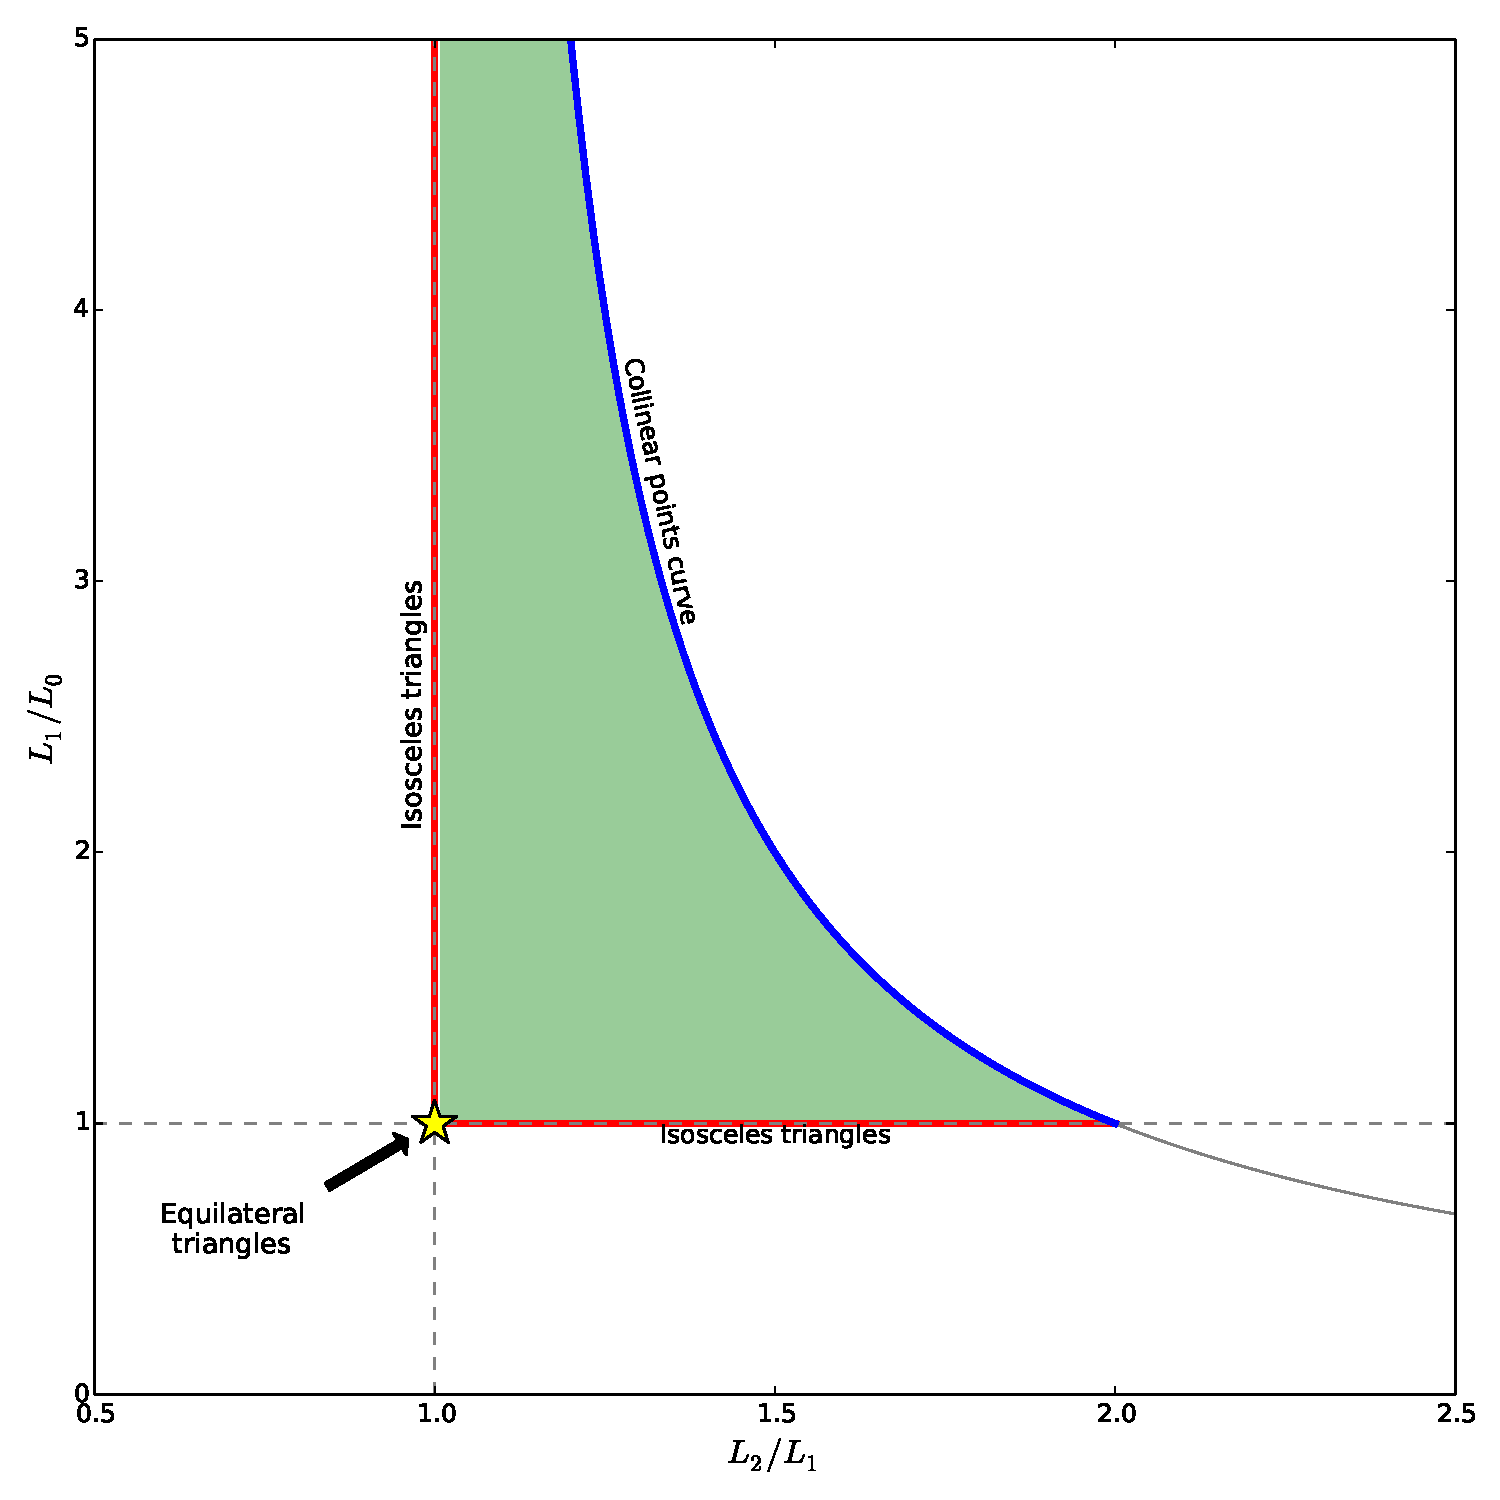
\includegraphics[scale=0.5]{figures/astroalign/invariantMap01.pdf}
   \caption{Range of the mapping for the astroalign invariants in equation \ref{invdef}.}
   \label{fig:inv_region}
\end{figure}

Other invariant mappings will have different mapped regions with potential better spatial distribution of the triangles on the invariant space.
But our choice of invariance proved to work successfully in the situations we need.


%Other invariant sets can be constructed, each with a particular mapping from the set of side lengths of triangles to a region in the 2D plane of invariants.

%Some other examples are given in figure \ref{fig:inv_maps}. These have been explored numerically plotting the invariants for a large number of triangles.

%\begin{figure}[htb]
%   \centering
%   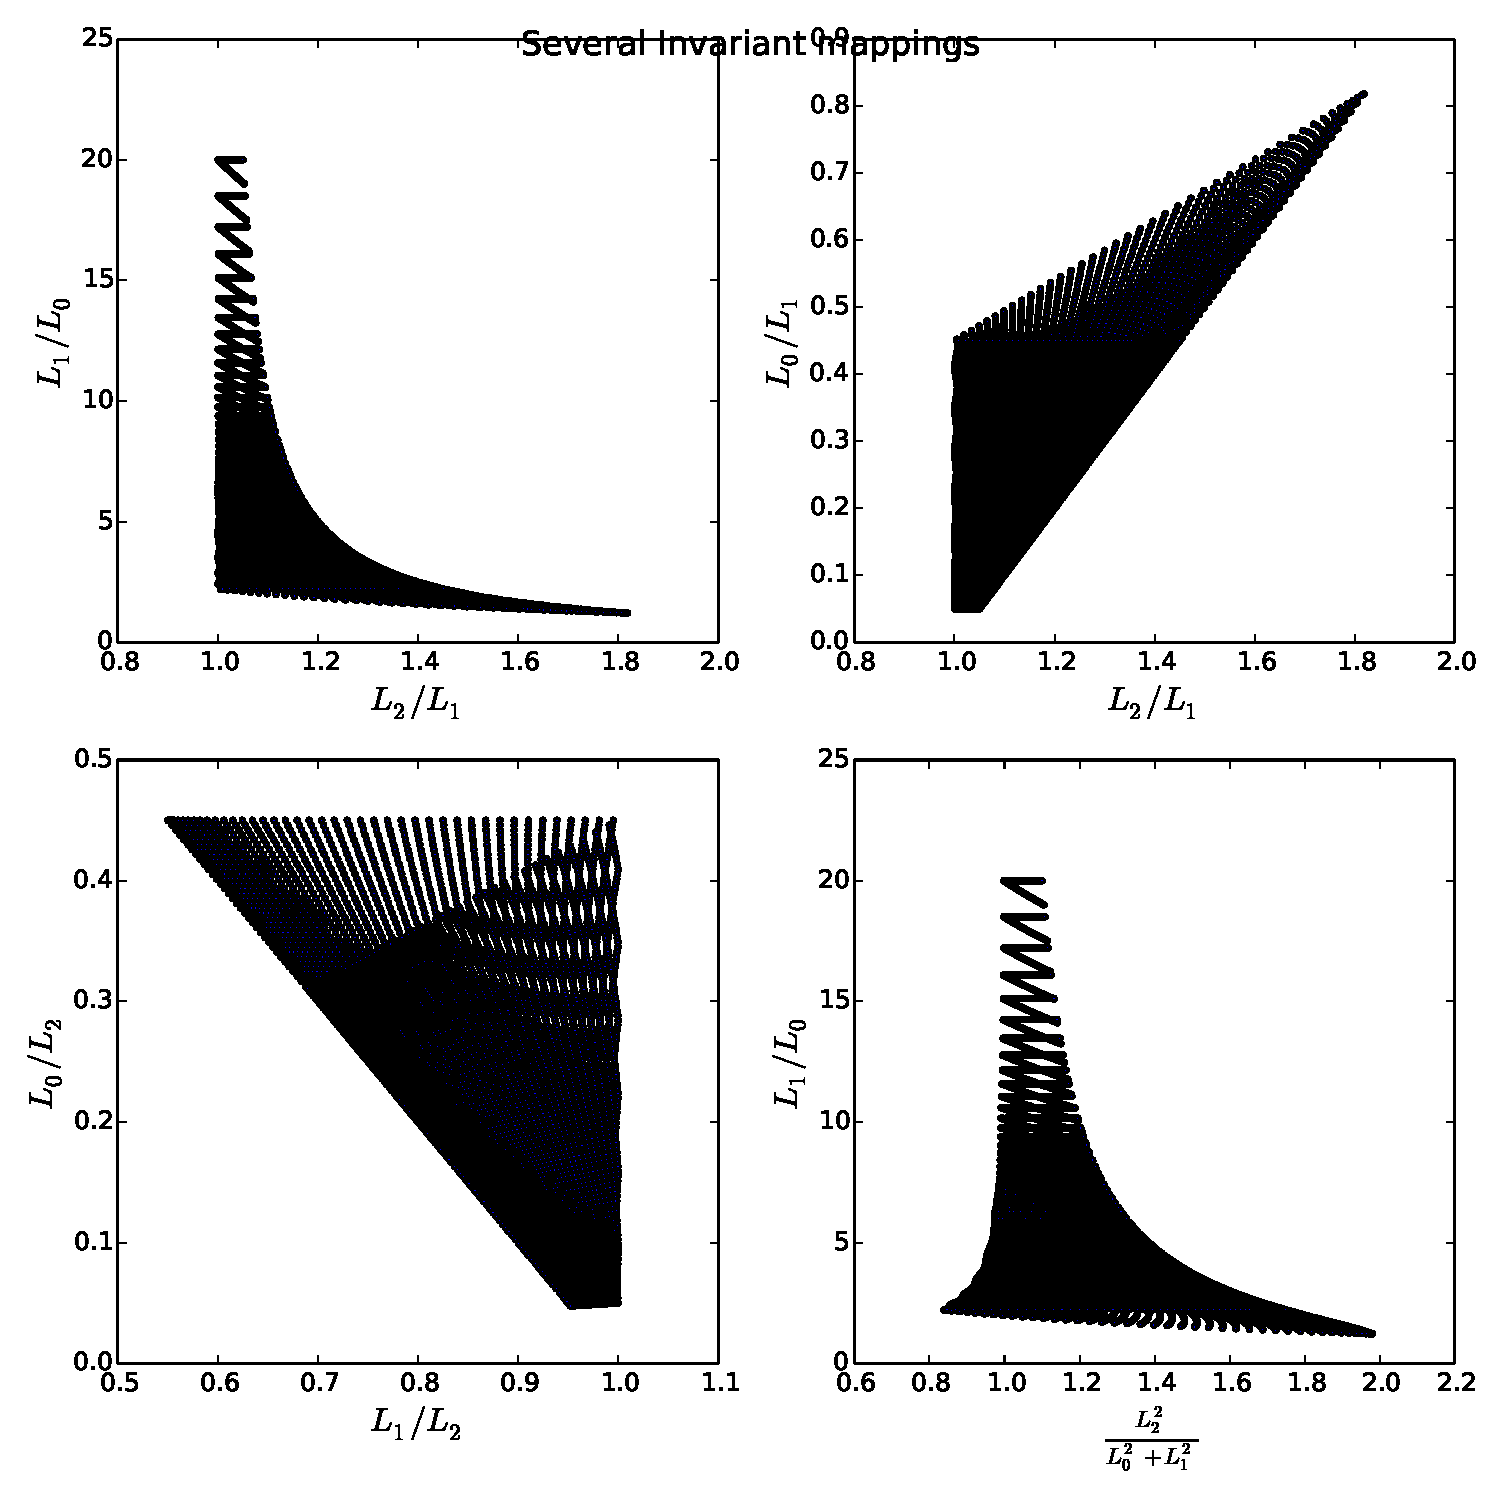
\includegraphics[width = \linewidth]{figures/astroalign/differentInvariantMaps.pdf}
%   \caption{Four examples of invariant mappings}
%   \label{fig:inv_maps}
%\end{figure}


\subsection{An Example}

Let's see how the algorithm performs on an ideal example.

For this, we create several stars at random positions and we rotate and translate them as seen in figure \ref{fig:ideal_sources}.

\begin{figure}[htbp]
   \centering
   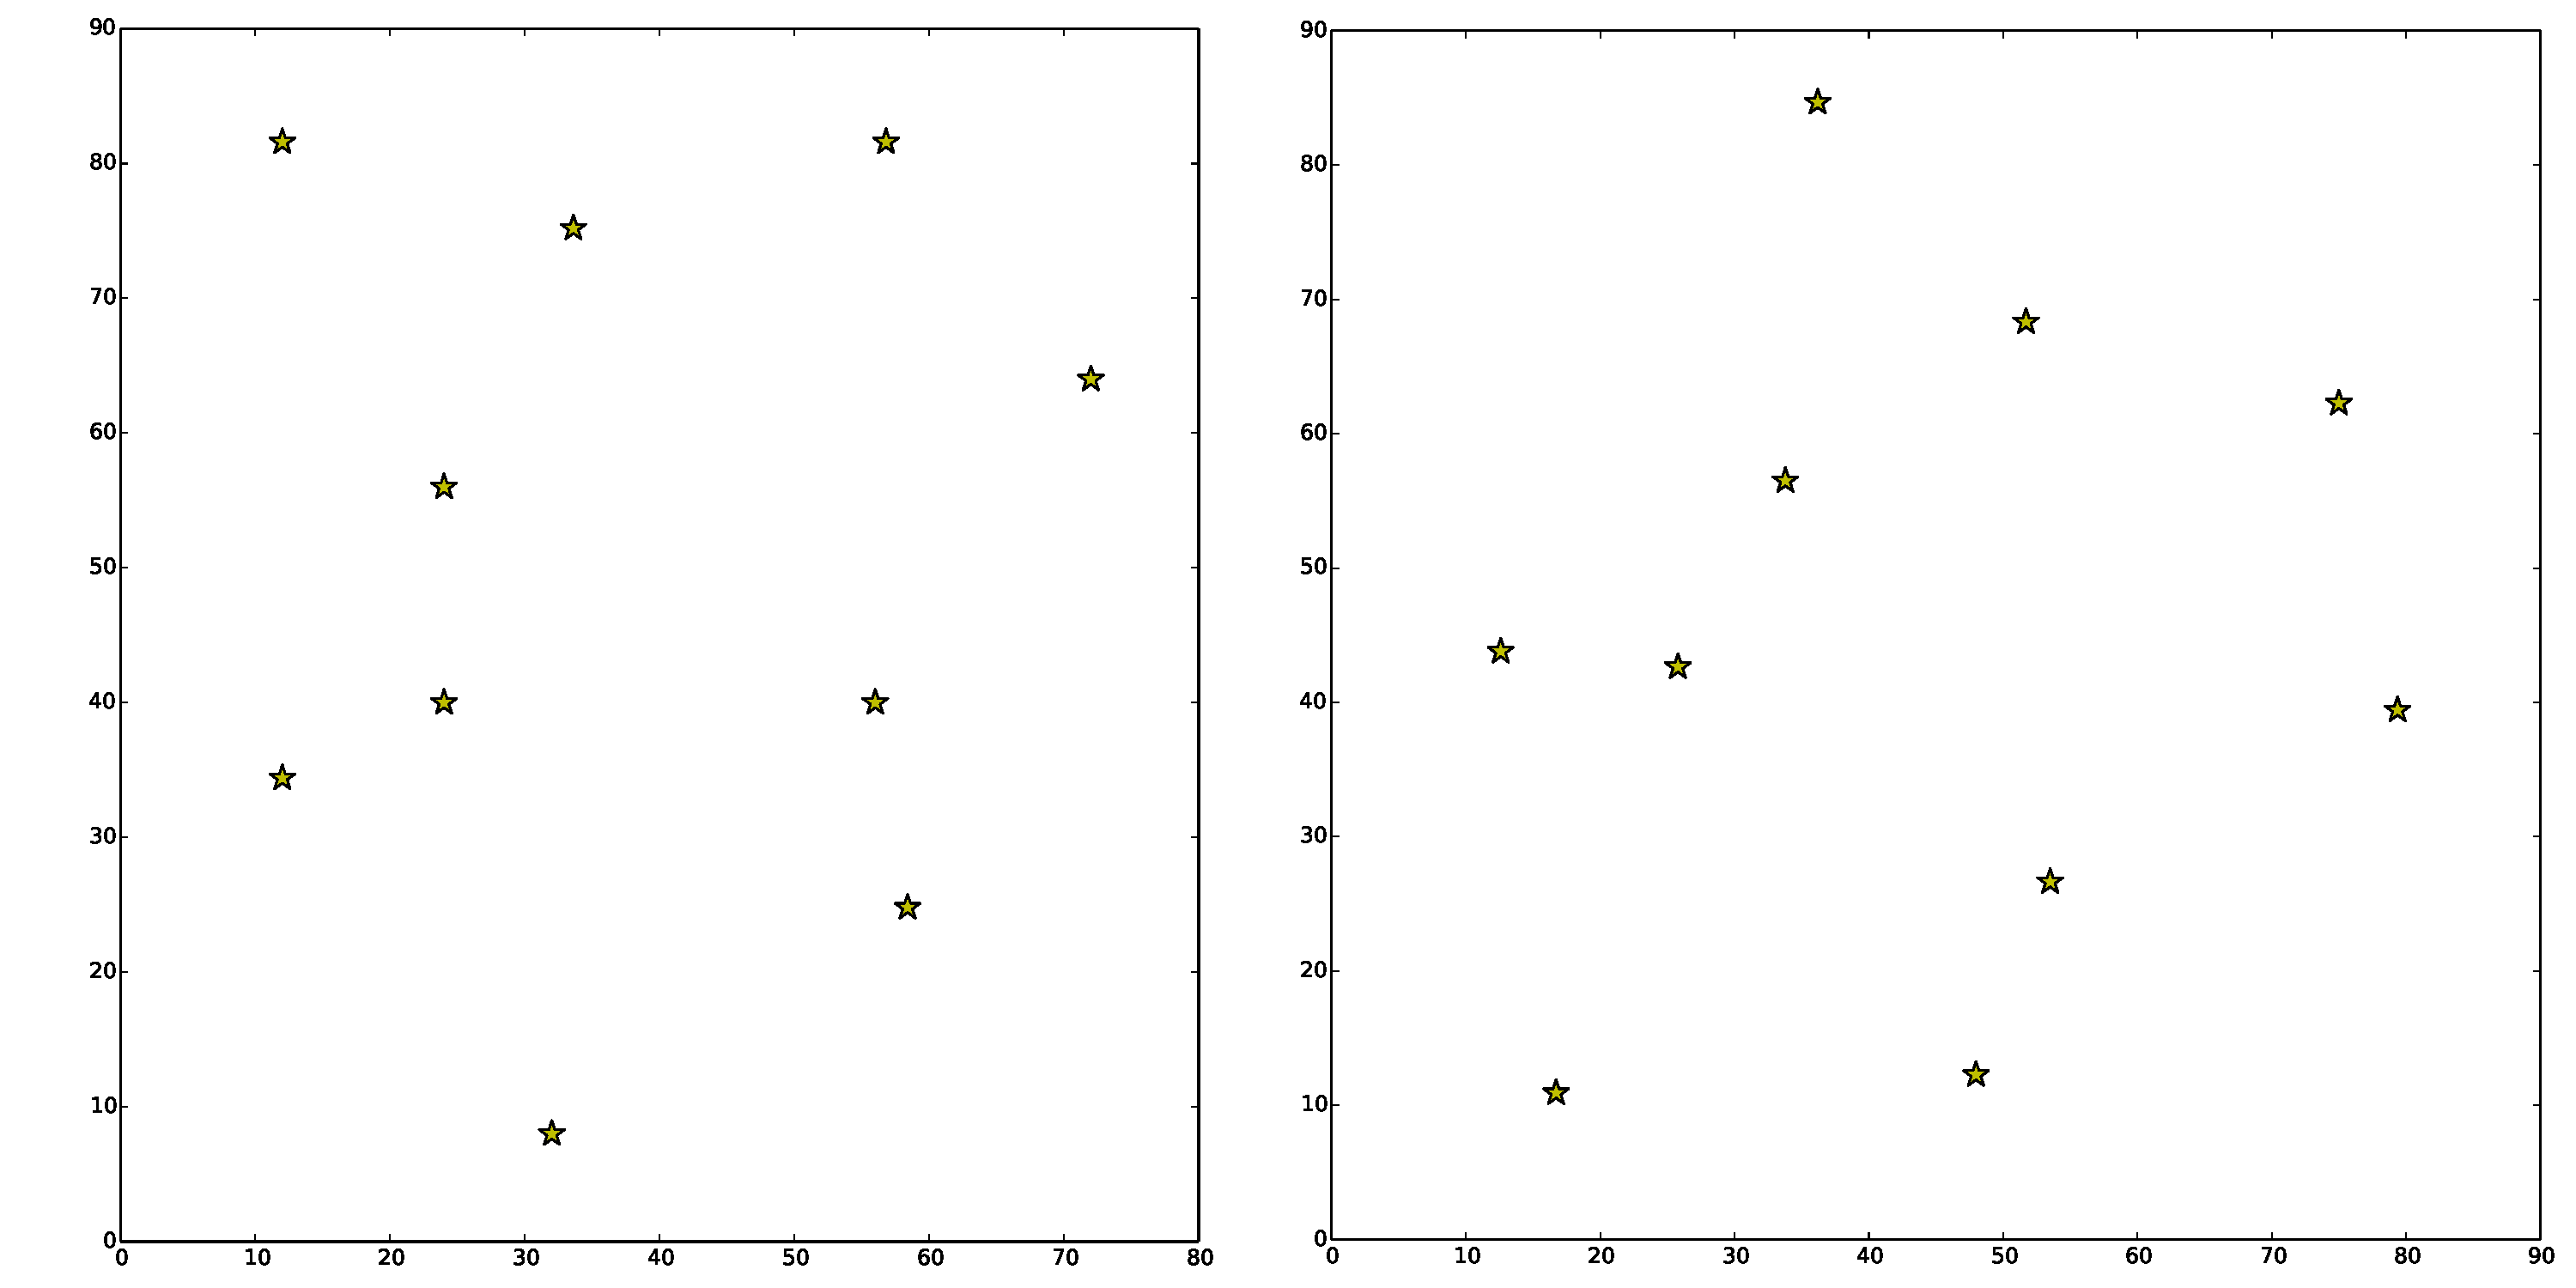
\includegraphics[width = \linewidth]{figures/astroalign/idealSources.pdf}
   \caption{Two ideal distribution of sources}
   \label{fig:ideal_sources}
\end{figure}

The invariant features in (\ref{invdef}) from this set of stars is plotted in figure \ref{fig:ideal_inv}.

\begin{figure}
   \centering
   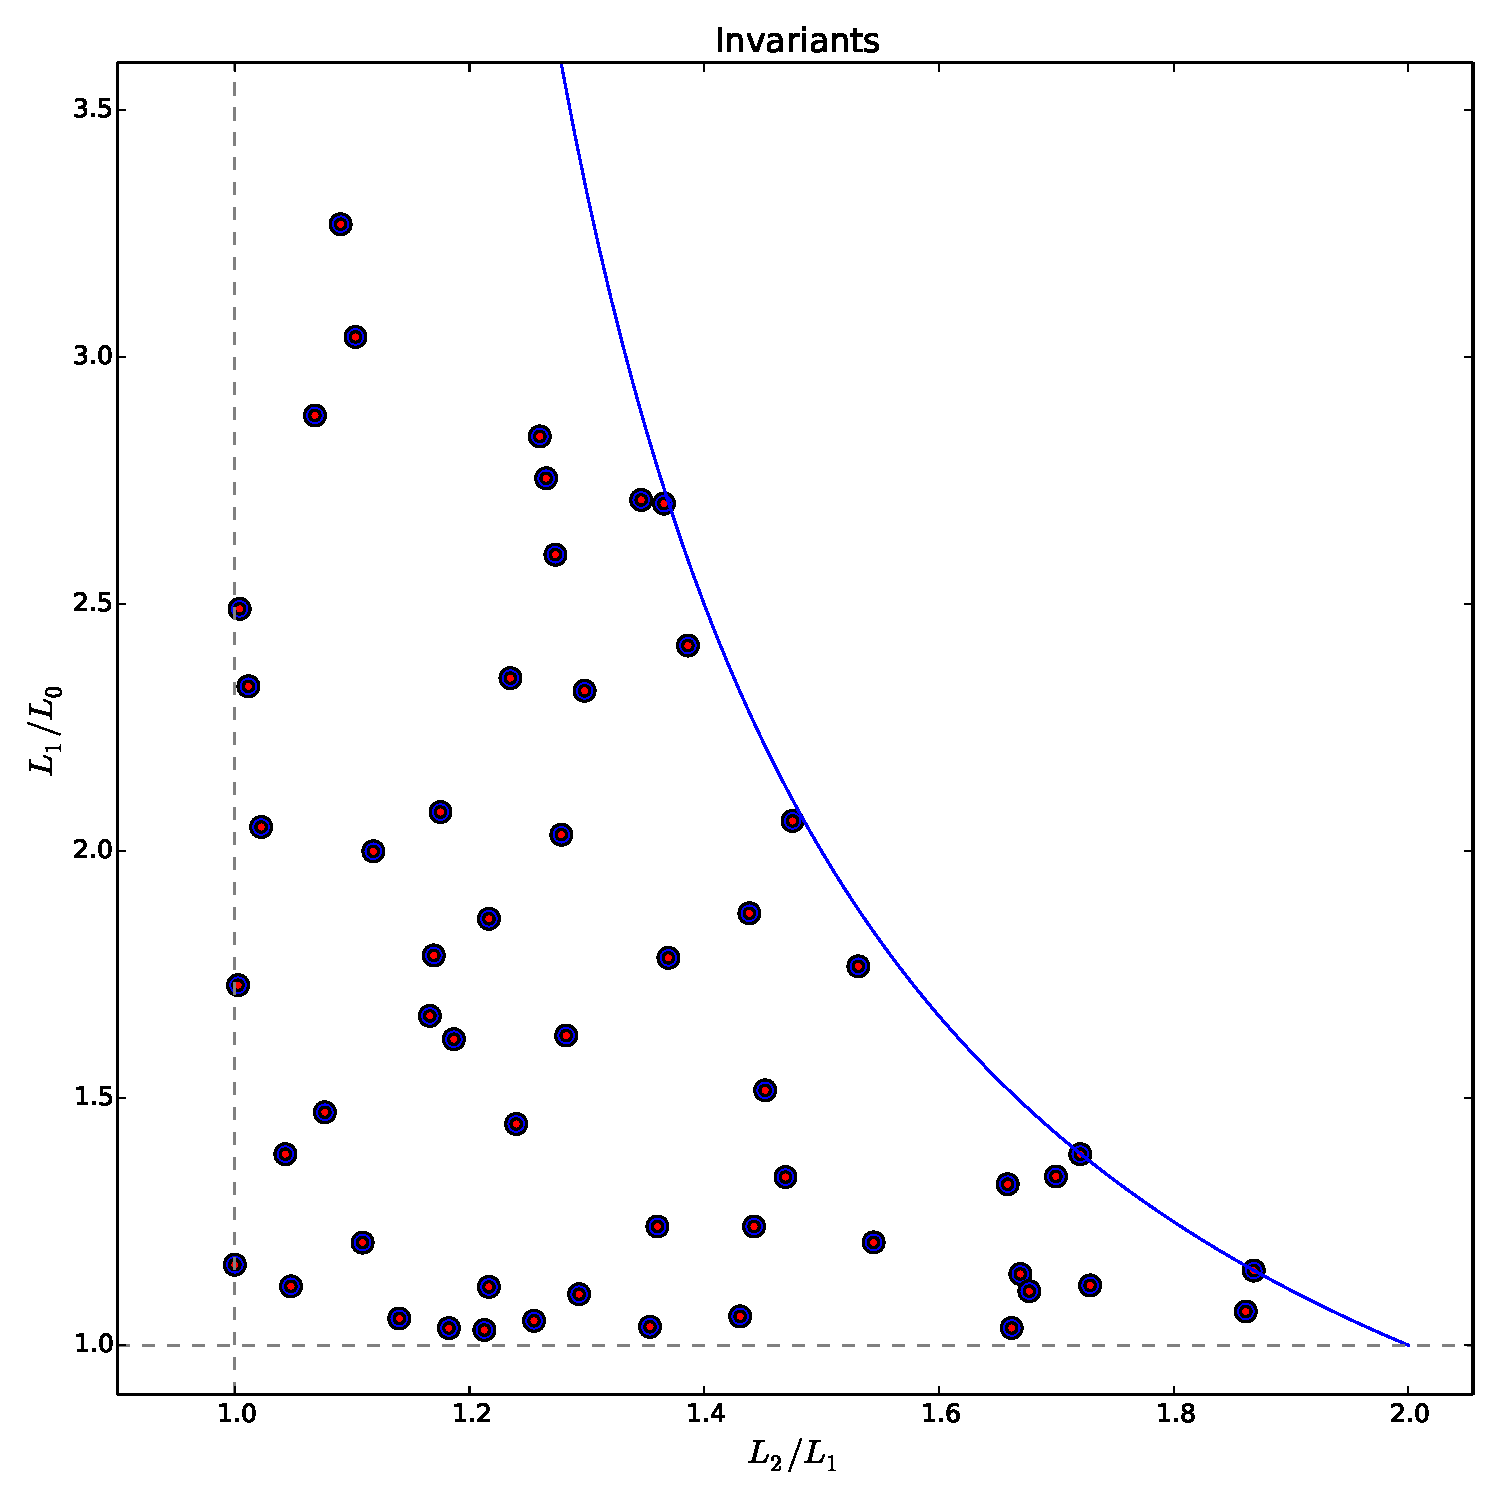
\includegraphics[scale=0.3]{figures/astroalign/idealInvariants.pdf}
   \caption{Invariants for the ideal example}
   \label{fig:ideal_inv}
\end{figure}

We note that some invariants belong to collinear points, and the distribution of points is fairly sparse. 
This will help the identification phase when we try to match our triangles.

In the figure, the invariant points for both images were plotted. They appear superimposed in the plot.

We note that every blue invariant point has its corresponding red invariant point on top. 
There are no points without a partner for neither of the images. 
This is because all the sources in one image appear in the other one, there are no missing stars.
In a real situation, some stars will be missing because they are out of the field of view or because they became too faint due to extinction or any other technical reason. 
The algorithm should still work with missing or extra stars in the reference or test image. 

Another issue with real images is that locating the position of a source is not entirely precise, so small errors will appear in the expected position of one source with respect to its partner in the other image.
This error in turn creates an error on the lengths of the sides of the triangle and thus on the invariants calculated from it.
In practice, the invariant points will lay close to each other to a given small tolerance.

Once we have the set of invariants from both images, we query a correspondence to the kd-tree for possible matches within a given tolerance radius. 
Each returned match will be a correspondence between a triangle in one image and another. 
From each, we can make the point to point correspondence, provided all sides are unequal, and this will determine a unique transformation between the images.

Some of the correspondences won't be real ones. It could be that by chance there are two similar triangles in the images that belong to different set of stars.

This is where the RANSAC algorithm comes in.

\subsection{The RANSAC algorithm}

From its Wikipedia page 

\emph{``The Random sample consensus (RANSAC) algorithm is an iterative method to estimate parameters of a mathematical model from a set of observed data which contains outliers.''}

In our case the mathematical model is the similarity transformation between both images and the parameters are those of the transformation, i.e. the rotation, translation and uniform scaling parameters.

RANSAC is capable of choosing a transformation that fits most of the other triangles and is not affected by the rest of spurious outliers. 

This algorithm is also used in the computer vision package OpenCV for a very similar purpose, to ignore outliers when trying to estimate an homography between two images. 

In our case we look for the parameters $t_x$, $t_y$ for the translation in the $x$ and $y$ direction, the rotation angle $\alpha$ and the dilation parameter $\lambda$.

The transformation applied to a point $(x,y)$ will look like this:

\begin{align*}
\left(
 \begin{array}{lll} 
 \lambda \cos \alpha & \lambda \sin \alpha& \lambda t_x \\
 - \lambda \sin \alpha & \lambda \cos \alpha& \lambda t_y \\
 0 & 0 & 1
 \end{array}
\right)
\equiv
\left(
 \begin{array}{lll} 
 a_0 & b_0 & c_0 \\
-b_0 & a_0 & c_1 \\
 0 & 0 & 1
 \end{array}
\right)
\end{align*}

To make our problem linear, we will consider the parameters $a_0, b_0, c_0, c_1$ as if they were independent.

Two data points pairs are sufficient to determine uniquely a transformation for this 4 parameters. 
More can be used if we use a linear square minimization.

%This candidate transformation $T$ will be tested against all the other triangle matches in a RANSAC algorithm.

\subsection{Error propagation}

Doing a simple propagation of errors we see that for nearly equilateral triangles $L_{1} \approx L_{2} \approx L_{3} \approx L$, 
the errors in the invariants go like $\Delta I_{i} \sim \frac{\Delta L}{L}$.
This means that, for invariants near $(I_{1}, I_{2}) = (1, 1)$ errors in the determination of the lengths of the triangle side will not magnify errors in the invariants.

\section{OIS Python Package} \label{section:ois}
	
Optimal Image Subtraction (\emph{ois}) is a Python module that implements several Difference Image Analysis methods as described in section \ref{section:dia}.
The math behind this implementation is explained in detail in Appendix \ref{appendix:dia}.

OIS works on Numpy arrays, so that way is agnostic on the origin of the image. 

Bad pixels that need to be ignored in the image are marked using Numpy's masked arrays (True on bad pixel).

The interface to the user has two entry points: the module methods optimal\_system and subtract\_on\_grid. 
The latter is just a convenient method to partition the image in a certain grid and perform the former on each grid, taking into account pixels outside the grid when necessary.

optimal\_system will return the difference image along with the optimal image to be subtracted (the ruined reference), the kernel of the convolution and the subtracted background.
optimal\_system and subtract\_on\_grid will return the same elements, but a list of kernels for each grid element instead of just one like the previous case.

OIS currently supports 3 different methods for subtraction: Alard-Lupton, Bramich, and Adaptive Bramich (an adaptive version of Bramich).

The documentation and usage for the code can be found in http://optimal-image-subtraction.readthedocs.io.
The source code is available in the TOROS GitHub repository at https://github.com/toros-astro/ois.
OIS is released under MIT License.

\section{Corral: The Pipeline Framework}

One particular problem about the implementation of the pipeline is the necessity of maintaining a large database for the astronomical observations.
Our current implementation of the pipeline lacks a database back-end to store and query past observations in an ordered manner.

Juan Bautista Cabral, a collaborator for the TOROS project, developed the Corral framework (\citet{2017Corral..B}) to ease in the building of the pipeline.
The framework is part of a separate project, following the SoC paradigm and can be installed via a pip command.

Starting a robotic observatory in the extreme environment of Cordon Macon, Argentina introduces serious challenges.
Given the isolation of this geographic location (the place is at \textasciitilde 4600 m above sea level and the closest town is 300 km away), 
it was clear that human interaction would be spotty at best and full internet connectivity may not be guaranteed.
This imposes strong demands on the pipeline data processing and storage to be in location, with failure tolerance arising as a key constrain feature.

To asses this issue, Corral provides the formalization of a pipeline framework based on the concepts of Steps and Models following the 
well known design pattern \textit{Model--View--Controller} (MVC) and built on top of a SQL Relational Database.

Every Model instance can be thought of a table in the database and represents a component or piece of data in the pipeline.
We can have a model for a light frame, a model for image stacks, a model for subtraction images, a model for a candidate of a transient, etc.
Models contain all the information relating a particular component, including its `status' within the pipeline process.
This helps when we want to inquire about unfinished processes or about a particular set of images.

Steps are the fundamental blocks of the pipeline, acting on the Model instances by doing the actual processing and updating their status on the database.
They can also create new Model instances and corresponding registers on the database.
The pipeline will execute the Steps consecutively when needed and will do parallel processing when allowed.

A special kind of Step, named Loader allows to initialize the database or load it from an external source to the pipeline.
The pipeline also allows for the creation of Alerts, which are special kind of steps raised by some particular state of the data stream.
When one of these is raised, it is compulsory an Alert will notify the research group as specified in the implementation.

The formalization of the pipeline into the Corral framework allows the developer to deal with the specifics of the manipulation steps 
without worrying about creating code for multi-processing workflow, coding architecture or code to interact with the database.
Working on the Corral framework has the additional perk of estimating a Quality Index for the code, and automatic documentation generation.

Source code for the project is hosted in the TOROS GitHub page \url{https://github.com/toros-astro/corral}.
Documentation and a tutorial to get started can be found in \url{http://corral.readthedocs.io/}.

\section{Winnow - Human classification of Real/Bogus}

Along with the broker website (see section \ref{section:broker}), the web server for the TOROS project hosts \emph{winnow}, 
an interactive Real/Bogus \emph{web-app} for human classification.
The website was developed using the Django web framework.

The website at \url{https://toros.utrgv.edu/winnow/}, is a web interface that presents users cut-outs of possible real transients.
The user votes on the categories `real' or `bogus' and is presented with the next cut-out.

This kind of `citizen science' has been popular and extremely useful in 
GalaxyZoo (see for example \citet{2008MNRAS.389.1179L}) and CitizenSky (\citet{2012POBeo..91..307T}).
The natural pattern recognition in humans is excellent. 
With little training, humans can look at an image of a subtraction field and determine quickly and accurately which are potential transients among the hundreds bogus artifacts.

The original idea for the website was to create a training set, using the power of community to label examples.
One of the hardest tasks in obtaining a good data set to train Machine Learning agents is labelling instances, 
since relevant astronomical transients on the sky can't announce themselves as such.

Winnow made use of a database to record the votes and even has an interface to admin users to retrieve the classification.
Earlier attempts to ML relied on sets of data generated by the contribution of undergraduate students at UT Rio Grande Valley.
Unfortunately, these data sets suffered from great class imbalance.
Winnow was a visual data mining tool, but due to the natural scarcity of real transients in the images, it was hard to extract the positive examples.

The imbalance of the training set could be mitigated by some techniques in ML, like oversampling, undersampling, bagging or SMOTE.
In particular, SMOTE gave the best results.

Even though the results achieved with humanly generated data sets were not ideal, winnow proved to be a useful tool for educational purposes.


%%%%%%%%%%%%%%%%%%%%%%%%%%%%%%%%%%%%%%%%%%%%%%%%%%%%%%%%%
%
%                              CONCLUSIONS
%
%%%%%%%%%%%%%%%%%%%%%%%%%%%%%%%%%%%%%%%%%%%%%%%%%%%%%%%%%
\chapter{Conclusions}

A multi-messenger project like TOROS --that was established to follow-up gravitational wave detections to find potential optical counterparts-- requires a fast responsive system to deal with the ephemeral nature of the transient events of interest.
Following this requirement, we developed software to immediately respond to GW alerts by triggering an automatic chain of processes.
Once we receive the alert the following processes are launched in order:

\begin{itemize}
\item Parsing the VOEvent alert file, capturing information and metadata for the detection.
\item Send email notifications to designated members of the collaboration, alerting of the new detection and providing relevant information about the event gathered in the previous step.
\item Download the skymap files for the localization uncertainty of the event.
\item Send skymap FITS and PNG files over email to designated members of the collaboration.
\item Process skymaps to create observation targets for each of the telescopes, based on criteria of potential host galaxy, visibility at the time of the event and the localization probability given by LIGO.
\item Upload the targets to a broker website to inform the participating telescopes the observation targets for the night.
\end{itemize}

If TOROS were a truly robotic observatory, the observations could be scheduled programmatically without human intervention,
and then automatically retrieved to perform the next stages of the pipeline.
The robotization of the telescope is the ultimate goal of TOROS, but at this time, the telescopes that participate in the collaboration are manually operated, in consequence the automatic flow of the pipeline is interrupted at this step.
Even without robotization, implementing transfer and storage protocols for the data would help in making a more automatic work-flow, but this is an issue that has not been resolved at the time of this writing. 

In spite of this technical issue, we also developed code that can be executed after the images are taken, to complete the stages of transient detection and recovery.
As we said, these subsequent steps are not triggered by any event, but have to be executed manually, once the images are received back from the telescopes.

The transient recovery is done with an Image Difference Analysis and a Machine Learning algorithm to rake over the sources present in the image to identify possible candidates.
We tested the algorithms in a data set of 626 images of the South Celestial Pole taken by the Chinese mission CSTAR.
The results of the simulation showed that 99.15\% of the simulated transients were recovered (the \emph{recall} score) and only 0.43% of the transients were misclassified subtraction artifacts.
It also shows that simple parameters of source extraction programs like SExtractor, and others derived from them, are sufficient to achieve acceptable levels of detection and minimum contamination, at least in this data set that we tested.

During the observational LIGO campaign of O1, TOROS participated in the follow-up search along with other 23 observatories.
The TOROS collaboration conducted a prompt search for the electromagnetic counterpart of the 
first gravitational wave event reported by LIGO in September 14, 2015, using the 1.5 m telescope of Estacion Astrofisica Bosque Alegre (EABA) in Cordoba, Argentina. This event was the first ever direct detection of a gravitational wave.

We observed for two consecutive nights immediately after we received the alert, searching on 14 targets in 21 fields containing nearby (D < 60 Mpc) luminous (MB <  21 mag) galaxies with high probabilities of hosting the event. 
We covered 0.62 square degrees which corresponds to an integrated probability of about 0.03\% in the cWB map and less than 0.01\% in the rest of the skymaps. We reached a 5$\sigma$ limiting AB magnitude of r = 21.7.

We applied to the images the same process than our mock run on the CSTAR data, with a-posteriori references images taken a few months after, in December 2015.
The Image Difference + Machine Learning analysis did not show any transient of astronomical origin.
The fact that we did not find any genuine transient in our search is not surprising given the small area surveyed (\textasciitilde 0.62 sq. degrees) 
and the low cadence of the observations (with only two epochs per target, separated by 73$\pm$3d). 

More importantly, our null results are consistent with the LIGO detection of a binary black hole merger, for which no optical EM counterpart is expected.


\appendix

\chapter{Derivation of the Gravitational Wave Equations} \label{gwderivation}

Gravitational waves are a particular kind of solution to the Einstein's field equations of General Relativity.

In many situations we can consider, we are in a flat background situation, in which our metric does not differ much locally from the Minkowski metric.
Suppose we are far away, removed from any strong source in an asymptotically flat spacetime.

In such situation we can assume that locally our metric is the Minkowski metric $\eta$ plus some small deviation $h$. We want to study the dynamics of such small perturbation in a linearized Einstein field equation. 


To do that, we consider the metric $g = \eta + h$ in the linearized Einstein's field equations. Linearized here means that quadratic and higher factors of $h$ will be simply ignored, as they are assumed much smaller than the flat metric.

Let's find out what condition the Einstein field equation $G_{\mu \nu}(\eta + h) = 8\pi T_{\mu \nu} = 0$ imposes on this small perturbation $h$.

%\begin{align}
%G_{\mu \nu}(\eta + h) = 8\pi T_{\mu \nu} = 0
%\end{align}

%It is worth noting here that Einstein equations are not linear in nature, but they are second order on the metric derivatives and furthermore linear on the second order terms. This will allow us to derive from the linearized Einstein equations, a second order wave equation on the small perturbation $h$ that decouples from $\eta$.

%Another issue to point out is that the vague definition of 'small perturbation' has to be of physical nature and not an artifact on the choice of the coordinate system. We will not worry about this issue on the present work, but it is worth keeping it in mind. Other concerns about coordinate system effects were historically raised and settled in time, particularly the many gauge choices done during the derivation.

The Christoffel symbols to first order in $h$ are:

\begin{align}
\Gamma_{abc} &= \frac{1}{2} \left( g_{ca,b} + g_{cb,a} - g_{ab,c} \right) \\
  &= \frac{1}{2} \left( (\eta + h)_{ca,b} + (\eta + h)_{cb,a} - (\eta + h)_{ab,c} \right) \\
 &=\frac{1}{2} \left( h_{ca,b} + h_{cb,a} - h_{ab,c} \right) 
\end{align}

At this point we must note that we will still call $g^{ab}$ the inverse of $g_{ab}$, which is $g^{ab} = \eta^{ab} - h^{ab}$ to first order in $h$. 

And thus,
\begin{align}
\Gamma^{a}_{bc} &= g^{cd} \Gamma_{abd} \\
 &=(\eta - h)^{cd} \Gamma_{abd} \\
 &= \frac{1}{2} \eta^{cd} \left( h_{ca,b} + h_{cb,a} - h_{ab,c} \right) + \order(h^2)
\end{align}

Similarly, the Ricci tensor to first order in $h$ will be:

\begin{align}
R_{ab} &= \Gamma^{c}_{ab,c} - \Gamma^{c}_{cb,a} \\
&= \frac{1}{2} \left( h_{a}{}^{c}{}_{,bc} + h_{b}{}^{c}{}_{,ac} - h_{ab,c}{}^{c} - h_{c}{}^{c}{}_{,ab} \right)
\end{align}

Which will finally lead us to the Einstein's tensor $G$:

\begin{align}
G_{ab} &= R_{ab} - \frac{1}{2}g_{ab}R \\
&= R_{ab} - \frac{1}{2}\eta_{ab}R + \order(h^2) \\
&= \frac{1}{2} \left( h_{ac,b}{}^{c} + h_{bc,a}{}^{c} - h_{ab,c}{}^{c} - h_{c}{}^{c}{}_{,ab} -\eta_{ab} \left( h_{cd,}{}^{cd} - h_{c}{}^{c}{}_{,d}{}^{d} \right) \right)
\end{align}

This can be brought to a shorter form defining $\bar{h}{}_{ab} = h_{ab} - \eta_{ab} h$

Where $h = h_{c}{}^{c}$ is the trace of the metric tensor $h$.
With this definition, the Einstein's field equation becomes:

\begin{align}
\bar{h}{}_{ab,c}{}^{c} + \bar{h}{}_{ac,b}{}^{c} + \bar{h}{}_{bc,a}{}^{c} -\eta_{ab} \bar{h}{}_{cd,}{}^{cd} = 0
\end{align}

\section{Gauge choices}

There is a gauge freedom in General Relativity corresponding to the group of diffeomorphisms, that can be used to simplify the equations even more. Just like the Gauge freedom in electrodynamics $A \rightarrow A + \partial \chi$ we can chose $h$ to satisfy $\bar{h}{}_{ab,}{}^{b} = 0$

In this ``Lorentz Gauge'', the linearized Einstein field equations, reduce to the usual wave equation for each component of $\bar{h}$:

\begin{align}
\bar{h}_{ab,c}{}^{c} = \Box{\bar{h}{}_{ab}} = 0
\end{align}

Further gauge choices can let us choose the trace of $\bar{h}$ to be zero and each $h_{0\mu}$ component to be zero for $\mu = 0,1,2,3$. Notice that once the trace of $\bar{h}$ is set to zero, it implies that $\bar{h}{}_{ab} = h_{ab}$

\begin{align} \label{gaugecond}
& \Box{h_{ab}} = 0 \\
& h_{ab,}{}^{b} = 0 \\
& h_{a}{}^{a} = 0 \\
& h_{0 \mu} = 0; \; \mu=0,1,2,3
\end{align}

This is called the transverse traceless (TT) gauge. The reader can refer the full derivation for the gauge choices in Misner or Wald.

With the conditions in (\ref{gaugecond}), we seek solutions in the form of plane waves of the form $h_{ab} = H_{ab}e^{\pm \imath k_{\mu}x^{\mu}}$.

Our gauge conditions impose similar conditions on $k$ and $H$:

\begin{align}
& k^{\mu} H_{\mu \nu} = 0 \\
& H_{\mu}{}^{\mu} = 0 \\
& H_{0 \mu} = 0; \; \mu=0,1,2,3
\end{align}

This leaves $H$ with only two independent components. If we consider a wave propagating in the z direction, the most general form for a transverse traceless metric will be:

\begin{equation}
\begin{bmatrix}
0 & 0 & 0 & 0 \\
0 & h_{+} & h_{\times} & 0 \\
0 & h_{\times} & -h_{+} & 0 \\
0 & 0 & 0 & 0 \\
\end{bmatrix}
e^{\pm \imath k_{\mu}x^{\mu}}
\end{equation}

and the total metric $g$

\begin{equation}
\begin{bmatrix}
-1 & 0 & 0 & 0 \\
0 & 1 + h_{+}e^{\pm \imath k_{\mu}x^{\mu}} & h_{\times} e^{\pm \imath k_{\mu}x^{\mu}} & 0 \\
0 & h_{\times} e^{\pm \imath k_{\mu}x^{\mu}} & 1 - h_{+}e^{\pm \imath k_{\mu}x^{\mu}} & 0 \\
0 & 0 & 0 & 1 \\
\end{bmatrix}
\end{equation}

The two independent polarizations are called ``h plus'' ($h_+$) and ``h cross'' ($h_{\times}$).



%%%%%%%%%%%%%%%%%%%%%%%%%%%%%%%%%%%%%%%%%%%%%%%%%%%%
%
%                            DIFFERENCE IMAGE ANALYSIS
%
%%%%%%%%%%%%%%%%%%%%%%%%%%%%%%%%%%%%%%%%%%%%%%%%%%%%

\chapter{Difference Image Analysis} \label{appendix:dia}

Searches for time-varying and position-changing objects are undertaken by comparing a reference image of a particular region of the sky with a second image taken at the moment in which we are interested. Ideally, the reference image is taken with the same telescope using the same filter and CCD. The two images have to be aligned pixel by pixel and then subtracted to reveal any changes in light.

To make a suitable subtraction of two images, one has to match the frames to exactly the same seeing. Image Difference is a technique to find a convolution kernel that best describes (in some minimization sense) the change in point spread function between the images. The idea is to degrade the good seeing image---our reference image---to match the seeing of our second image. Finding the proper kernel can be a delicate operation and there's plenty of literature on the subject. Methods range from PSF modeling through common Gaussian profiles to unmodeled PSF's to Information Theory and Fourier Domain.

The first attempts at image subtraction relied on Fourier decomposition of the images, 
but the technique suffered when noise levels were even moderate and the results were not always good.
\citet{1998ApJ...503..325A} were the first to propose a solution in image space (as opposed to Fourier space). 
They also summarize previous efforts in their introduction and references therein. 
In that paper, they propose an optimization problem that we describe briefly as follows.

We have an image $I$ and a reference image $R$, for which we want to find a convolution kernel $K$ such that

\begin{align}
I(x,y) & \approx (R \mathbin{*} K)(x,y) \\
 & \approx \int \mathrm{d}u \mathrm{d}v {R (u,v) K(x-u,y-v)}
\end{align}
 
The integral symbol has to be understood in practice, as a sum over all the pixels $(x,y)$ on the image. 

The kernel $K$ will try to correct for the PSF difference between the two images.
It's worth noting here, that even though it could be practical to the reader to think so, the kernel $K$ is neither the PSF of the reference nor the PSF of the image.

Usually, the reference image is the one with the best {\em seeing}, 
because it can be done by median-stacking good images, or using Lucky Imaging [add ref] or some other method.

To convert the problem into a linear one, we decompose the kernel into a linear combination of ``{\em basis}'' functions $B$.

\begin{equation} \label{kernel_linear}
K(u,v) = \sum_{i} a_{i} B_{i}(u,v)
\end{equation}

These $B_{i}$ could in principle be any reasonable set of functions. 
%The two most popular choices are modulated Gaussians and the Delta basis, which will be explained in further detail in section \ref{basis}.

Using this linear combination, the convolution will be

\begin{align}
(R \mathbin{*} K)(x,y) & = \sum_{i} a_{i} \left( R \mathbin{*} B_{i} \right)(x,y) \\
 & \equiv \sum_{i} a_{i} C_{i}(x,y)
\end{align}

where the last line defines $C_{i}(x,y)$.

With this decomposition, we can find the set of $a_{i}$ that minimizes the square difference over all pixels.
Define a cost function $Q$:

\begin{align}
Q &= \int \left( I(x,y) - (R \mathbin{*} K)(x,y) \right)^2 \\
 & = \int \left( I(x,y) - \sum_{i} a_{i} C_{i}(x,y) \right)^2,
\end{align}

and let's minimize $Q$ over the set of $a$'s:

\begin{align}
\frac{\partial Q}{\partial a_{i}} = & 2 \int \left( I(x,y) - \sum_{j} a_{j} C_{j}(x,y) \right) C_{i}(x,y) 
\end{align}

Setting the last equation to zero, gives us:

\begin{align}
\sum_{j} a_{j} \int \left( C_{j}(x,y)  C_{i}(x,y) \right) =  \int I(x,y) C_{i}(x,y) 
\end{align}

Which we can write more succinctly as a matrix equation:

\begin{align} \label{matrix_eq}
\sum_{j} M_{ij} a_{j}  =  b_{i}
\end{align}

where

\begin{align} \label{matrix_def}
M_{ij}  &=   \int  C_{i}(x,y)  C_{j}(x,y) \\
b_{i} &=  \int I(x,y) C_{i}(x,y)  \nonumber
\end{align}

We can find the coefficients $a_{i}$ of the optimal kernel for the subtraction by inverting the system \eqref{matrix_eq}.

\section{Different basis functions}

As stated above, any choice of basis in the linearization \eqref{kernel_linear} could work, but two particular choices are the most popular.

The first one was proposed by \citet{1998ApJ...503..325A} and it consist of modulated centered Gaussians:

\begin{equation}
B_{n,d_n^{x}, d_n^{y}}(u,v) = e^{-(u^2+v^2)/2 \sigma_n^2} \times u^{d_n^{x}} v^{d_n^{y}}
\end{equation}

where the exponents in $u$ and $v$ add at most up to $D$, the degree of the modulation polynomial.

This choice of linearization gives enough freedom to approximate the kernel as a sum of modulated Gaussians, which is suitable for many situations.
The parameter $\sigma_n$ in each Gaussian is fixed beforehand by the user.

The number of Gaussians used in the expansion is given by $n$, and for each one of them we have $(D_n + 1)(D_n + 2)/2$ terms in the modulating polynomial.
That gives a total of $n(D_n + 1)(D_n + 2)/2$ unknown $a_i$ coefficients to solve for.

A simpler basis was proposed by \citet{2008MNRAS.386L..77B} and it's effectively a Dirac Delta function for each pixel.

\begin{equation}
B_{i}(x,y) = \delta(x-i,y-j)
\end{equation}

This choice of basis makes every pixel value in the kernel be determined independently by the minimization process.
Obviously, this allows for a greater variety of kernels than in the Gaussian case.
It also comes at a cost: now the number of unknowns to invert for grows quadratically with the kernel side length.
For a kernel of side 11 pixels, we have to create a matrix 121$\times$121 and then invert it. 

As we will see at the end of the chapter, even calculating the elements of the matrix to invert is an expensive operation,
so this absolute freedom in the kernel shape comes at the cost of a much higher numerical complexity.

Despite this complexity, the Delta basis can account for situations that the Gaussian basis can't address.
For example, if the images are very similar in PSF, then the compensating kernel of our problem should be an actual delta at the center 
---the identity kernel---or a very peaky function.

Bramich's method can actually return the correct kernel, while the Gaussian method will have trouble adjusting (potentially broad) Gaussians.

Another issue that Delta basis corrects very well is for tiny misalignments between our reference image and the image we are processing.
In fact, translations are included in the set of convolutions represented by displaced deltas on the kernel.
Convolving with a kernel with a delta displaced $(\Delta x, \Delta y)$ pixels away from the center will effectively translate the image by that same amount,
so misalignments due to small translations (the order of the kernel side) can be completely accounted for in the Delta basis.

\section{Add a varying background}

Background variation can be treated separately or simultaneously with the PSF fitting.

\subsection{Independent background estimation}

An independent background estimation can be done on each separate image before doing the PSF match.

For a stellar field image, one can create an image $I_{B}$, from the image $I$ by excluding all pixels above a certain threshold on the background noise. This image $I_{B}$ will contain pixels belonging to the background only (sources removed).

\begin{equation}
I_{B}(x,y)  = \left\{ I(x,y) : |I(x,y) - \mu| < \sigma \right\}
\end{equation}

On this image $I_{B}$, find the best polynomial fit of degree $d$ to the image using a least square fit.

Minimizing $Q$ over the $b_{ij}$ coefficients

\begin{equation}
Q = \int \left( I_{B}(x,y) - \sum_{i,j}^d b_{ij} x^i y^j \right) ^2
\end{equation}

will give the best polynomial fit to the background.

\subsection{Simultaneous PSF and background estimation}

To do it simultaneously with the PSF matching, we simply add it to our previous $Q$. This will let us remove any remaining variation on our new image $I(x,y)$.

\begin{align}
I(x,y) & \approx (R \mathbin{*} K)(x,y) + B(x,y) 
\end{align}

Note however, that this $B$ is not the sourceless image $I_{B}$ defined in the previous section. This $B$ represents the optimal background approximation that can be expanded as a polynomial with unknown coefficients.

$Q$ is defined now as

\begin{align}
Q &= \int \left( I(x,y) - (R \mathbin{*} K)(x,y) - B(x,y) \right)^2 \\
 & = \int \left( I(x,y) - \sum_{i} a_{i} C_{i}(x,y) - \sum_{i} b_{i} x^i y^j \right)^2
\end{align}

We can pile up the $b$ coefficients onto a larger set of $a$'s and define new $C$'s accordingly.

\begin{equation}
C_{i}(x,y)  = \begin{cases} 
(R \mathbin{*} K)(x,y)  &\mbox{when i,j refer to kernel}  \\ 
x^i y^j & \mbox{when i,j refer to background}  
\end{cases} 
\end{equation}

This leads us to the exact same (but extended) solution for the coefficients $a$, namely:

\begin{align}
\sum_{j} M_{ij} a_{j}  =  b_{i}
\end{align}

where

\begin{align}
M_{ij}  &=   \int  C_{i}(x,y)  C_{j}(x,y) \\
b_{i} &=  \int I(x,y) C_{i}(x,y) 
\end{align}

as before.

\section{How to deal with bad pixels} \label{badpixels}

The astronomical images can have pixel defects due to CCD defects or missing data from alignment. 
Those pixels can, in principle, be in both the reference frame $R$ and the new image $I$. 

Although it is advisable to use a reference image $R$ with few to none bad pixels for the reason that will be explained further on this section.

As before, we now want to approximate the two images as follow

\begin{align}
I(x,y)\bigg|_{\Omega} & \approx (R \mathbin{*} K)(x,y)\bigg|_{\Omega}
\end{align}

But this time, we want to restrict the above only for the good pixels in the images.

Bad pixels in $I$ and $R$ have to be excluded, but we also have to exclude those pixels in $R$ that {\em use} bad pixels in the convolution. This equivalent to dilate the bad pixels mask in $R$ with a kernel the same shape as the convolution kernel $K$. For this reason, it's better to have few bad pixels in $R$.

The union of the bad pixel mask from $I$ and the dilated bad pixel mask from $R$ is the common bad pixel mask. We call $\Omega$ to its complement, so that $\Omega$ is the set of good pixels that will be used in the subtraction. Pixels outside $\Omega$ will be tainted by the bad pixels in either of the two images.

This modification will now makes us define a new $Q$:

\begin{align}
Q = \int_{\Omega} \left( I(x,y) - (R \mathbin{*} K)(x,y) - B(x,y) \right)^2
\end{align}

That only differs from the previous one by the domain of integration (or sum).
The definitions for $M$ and $b$ are similarly derived:

\begin{align}
M_{ij}  &=   \int_{\Omega}  C_{i}(x,y)  C_{j}(x,y) \\
b_{i} &=  \int_{\Omega} I(x,y) C_{i}(x,y) 
\end{align}

\section{Dealing with large fields of view}

When dealing with large field of views, a simple solution suggested by Bramich 2010, is to partition the image into grids, and apply Image Differencing on each grid element.

Another solution is to include in the derivation, a space-varying kernel.
This has the advantage of addressing the issue directly, but we have to quit to the niceties of having convolutions done with FFT.

The derivation follows the usual least squares derivation, except this time we consider each kernel basis element modulated by a polynomial variation across the image. Following Miller (2008):

\begin{align}
K(u, v) &= \sum_n a_n(x,y) B_n(u, v) \\
&= \sum_{n,i,j} a_{nij} x^i y^j B_n(u, v)
\end{align}

The new equations for $M$ and $b$ as in \ref{matrix_def} are the same, except that $C_{i}$ is now defined as:

\begin{equation}
C_I = \left( R \mathbin{*} x^i y^j B_n \right) (x,y)
\end{equation}

and $I$ is here the collective index $\{n,i,j\}$.
Notice that the last equation involves an unusual type of ``convolution'' where the kernel is not constant. This prevents the use of FFT to speed up the calculation.

\section{Cost of building matrix M and b}

Recall that we have to solve the system of equations \eqref{matrix_eq} with definitions in \eqref{matrix_def}.

This implies that each component of the matrix $M$ will involve a convolution and an integration over the whole image.

Therefore, not only the inversion problem is expensive, but even calculating the matrix can be an expensive operation.

\pagebreak{}

\bibliographystyle{aa}
% was: \bibliographystyle{plain}
\nocite{*}
\bibliography{mybiblio}

\begin{vita}

Martin Beroiz was born in Argentina and completed his Bachelor degree in Physics in 2007 in the National University of Cordoba.
He moved to the United States in 2008 to start a Master program at the University of Texas at Brownsville (UTB), in the border city of Brownsville, Texas, where he resided for over 7 years.

In his Master program, Martin Beroiz studied Rotating Radio Transients (RRATs), a type of erratic pulse emission with similar characteristics to radio pulsar emission,
but transient in nature. The work was under the supervision of Dr. Jenet and in collaboration with a team at the Jet Propulsion Laboratory of NASA in California. 
This research resulted in two publications in the IEEE Journal on `` A Prototype Radio Transient Survey Instrument for Piggyback Deep Space Network Tracking''.

After completion of the Master program at UTB, he returned to the United States in 2010 for a doctorate in Physics in a Collaborative Program between UTB and UT San Antonio.
During this time, Martin Beroiz worked with Dr. Richard Price first, and later with Dr. Mario Diaz in the TOROS project.

His current interests include General Relativity, Particle Physics but also Software Engineering, in particular algorithms, simulations and web development.

He will in the future keep working on the TOROS project, perfecting the software and training newcomer students.

\begin{comment}
\section*{Education}

\begin{itemize}
  \item B.S. Physics, National Cordoba University (Argentina), 2007.
  \item M.S. Physics, University of Texas at Brownsville, 2010.
\end{itemize}

\section*{Publications}

\begin{itemize}
\item \href{https://arxiv.org/abs/1701.05566}{\bf Corral Framework: Trustworthy and Fully Functional Data Intensive Parallel Astronomical Pipelines} (2017) Juan B. Cabral, Bruno Sanchez, Martin Beroiz, Mariano Dominguez, Marcelo Lares, Sebastian Gurovich, Pablo Granitto; {\it submitted to Astronomy and Computing}.
\item \href{http://adsabs.harvard.edu/abs/2016ApJ...828L..16D}{\bf GW150914: First search for the electromagnetic counterpart of a gravitational-wave event by the TOROS collaboration} (2016). Mario C. Diaz et al; {\it The Astrophysical Journal Letters}, Volume 828, Issue 2, article id. L16, 6 pp.
\item \href{http://adsabs.harvard.edu/abs/2016ApJ...826L..13A}{\bf Localization and broadband follow-up of the gravitational-wave transient GW150914} (2016). B. P. Abbott et al. {\it The Astrophysical Journal Letters}, Volume 826, Issue 1, article id. L13, pp
\item \href{http://www.math.unm.edu/~lau/DMS1216866/tauFluids_BHLP.pdf}{\bf Multidomain, sparse, spectral-tau method for helically symmetric flow} (2014). M Beroiz, T Hagstrom, SR Lau, RH Price; {\it Computers and Fluids}  (2014), pp. 250-265.
\item \href{http://iopscience.iop.org/1538-3881/147/5/100}{\bf Bright microwave pulses from PSR B0531+21 observed with a prototype transient survey receiver} April 2014. J. Andrew O'Dea, F. A. Jenet, Tsan-Huei Cheng, Chau M. Buu, Martin Beroiz, Sami W. Asmar, and J. W. Armstrong; {\it Astronomical Journal}, 147, 100.
\item \href{http://ieeexplore.ieee.org/xpls/abs_all.jsp?arnumber=5555950}{\bf A Prototype Radio Transient Survey Instrument for Piggyback Deep Space Network Tracking}, May 2011. Chau M. Buu, Fredrick A. Jenet, John W. Armstrong, Sami W. Asmar, Martin Beroiz, Tsan-Huei Cheng, and J. Andrew O'Dea; {\it Proceedings of the IEEE} Volume 99, Number 5.
\item \href{http://journals.aps.org/prd/abstract/10.1103/PhysRevD.76.024012}{\bf Gravitational instability of static spherically symmetric Einstein-Gauss-Bonnet black holes in five and six dimensions}, 2007. M. Beroiz, G. Dotti y R.J. Gleiser, {\it Physical Review D} 76, 024012 hep-th/0703074.
\end{itemize}


\section*{Scientific Meetings and Conferences}

\begin{itemize}
\item \href{http://adsabs.harvard.edu/abs/2016APS..APRR14005B}{Speaker at the APS April Meeting 2016}, abstract R14.005. "Results of optical follow-up observations of advanced LIGO triggers from O1 in the southern hemisphere". South Lake City, April 2016.
\item \href{https://conference.scipy.org/scipy2014/schedule/presentation/1730/}{SciPy Conference 2014. Speaker at Mini Symposium in Astronomy}. "Transient detection and image analysis pipeline for TOROS project". Austin July 2014.
\item Advances and Challenges in Computational General Relativity, Brown University, Providence, RI, May 20-22, 2011.
\item Poster presentation 215th American Astronomical Society (AAS) Meeting, Washington DC, January 3-7, 2010 ``The X-ray Emission of SN1978K: Still Here After All These Years''  - Eric M. Schlegel, M. Beroiz.
\item Poster presentation 215th American Astronomical Society (AAS) Meeting, Washington DC, January 3-7, 2010 ``Current Results at PALFA Pulsar Survey at Arecibo Observatory'' - M. Beroiz, K. Stovall, F. Jenet, J. Cordes, D. Lorimer, D. Backer, PALFALFA Consortium.
\item Summer Provost Research Program at UTSA, 2009. Research on X-ray spectrum of Super Nova 1978K and Poster Presentation.
\item UTB Summer School in Gravitational Wave Astronomy at South Padre Island TX, June 2008.
\item Grav07, La Falda (Cordoba), Argentina. November 5-7, 2007.
\item Poster Presentation at 92nd AFA (Physics Association Argentina) Annual Meeting, Salta, Argentina, September 24-27, 2007.
\end{itemize}
\end{comment}

\end{vita}

\end{document}
